\documentclass[12pt,DIV14,BCOR12mm,a4paper,footinclude=false,headinclude,parskip=half-,twoside,openright,cleardoublepage=empty,toc=index,bibliography=totoc,listof=totoc]{scrreprt}
% encoding needs to be defined here, otherwise umlauts on the titelpage won't work.
\usepackage[utf8]{inputenc}
\usepackage{acronym}
\usepackage{setspace}
\usepackage{textgreek}
\usepackage{enumitem}
\usepackage{algorithm}
\usepackage{algorithmic}
% \usepackage{algpseudocode}
\usepackage{graphicx}
\usepackage{subcaption}
\usepackage{adjustbox}
\usepackage{makecell}
\usepackage{amsmath}
\usepackage[abbreviations,symbols,style=index]{glossaries-extra}
\usepackage[acronym]{glossaries}
\usepackage{abstract}
\usepackage[sorting=none]{biblatex}
\addbibresource{refs.bib}
%
%
%
% *****************************************************************
% -------------------> document preferences here <-----------------
% *****************************************************************
% Uncomment the settings you like and comment the settings you don't
% like.

% Language: 
% affects generic titles, Figure term, titlepage and bibliography
% (Note:if you switch the language, compile tex and bib >2 times)
\def \doclang{english} 	% For theses/reports in English
%\def \doclang{german} 		% For theses/reports in German

% Hyperref links in the document:
\def \colortype{color} % links with colored text
%\def \colortype{bw} 	% plain links, standard text color (e.g. for print)
%\def \colortype{boxed} % links with colored boxes
% *****************************************************************
%
%
%
% *****************************************************************
% --------------> put student information here <------------------
% *****************************************************************
% Please fill in all items denoted by "to be defined (TBD)"
\def \deworktitle{Raytracing-Kanalsimulation für Millimeterwellen-Innenraumlokalisierungssystem}        % German title/translation
\def \enworktitle{Ray tracing channel simulation for millimeter wave indoor localization system}        % English title/translation
\def \tutor{Sven Hinderer}
\def \student{Zheming Yin}
\def \worksubject{Forschungsarbeit S1462}  % type and number (S/Dxxxx) of your thesis
\def \startdate{01.01.2024}
\def \submission{30.06.2024}
\def \signagedate{30.06.2024}   % Date of signature of declaration on last page
\def \keywords{Radar system, Ray tracing, Radiation pattern, RCS}
% \def\abstract{This thesis uses ray tracing to build a tool chain in an indoor environment to calculate the channel impulse response (CIR) and receive signal of a autonomous mobile robot (AMR) at a given position and velocity. The room model is built in Blender and imported into Matlab's ray tracing to combine with the radar model, as well as adding more realistic antenna radiation patterns and radar cross-section (RCS) to observe whether the required information can still be accurately obtained in the range Doppler map and CFAR detection in a relatively larger and more realistic environment.}

% *****************************************************************
%


\usepackage{amsmath}
\usepackage{amsfonts}
\usepackage{ifthen}
\ifthenelse{\equal{\doclang}{german}}{
	\usepackage[ngerman]{babel} %german version
	\def \maintitle{\deworktitle}
	\def \translatedtitle{\enworktitle}
	% set , to decimal and . to thousands separator, if German language is used
	\DeclareMathSymbol{,}{\mathord}{letters}{"3B}
	\DeclareMathSymbol{.}{\mathpunct}{letters}{"3A}
	}{
	%english version
	\def \maintitle{\enworktitle}
	\def \translatedtitle{\deworktitle}
	}
\usepackage{txfonts} % Times-Fonts
\usepackage[T1]{fontenc}
\usepackage{color}
\usepackage[headsepline]{scrlayer-scrpage} % Headings

\usepackage{graphicx}
\usepackage[format=hang]{caption}       % for hanging captions
\usepackage{subfig}                     % for subfigures
\usepackage{wrapfig}                    % for figures floating in text, alternatively you can use >>floatflt<<
\usepackage{booktabs}                   % nice looking tables (for tables with ONLY horizontal lines)

%%%%% Tikz / PGF - drawing beautiful graphics and plots in Latex
% \usepackage{tikz}
% \usetikzlibrary{plotmarks}              % larger choice of plot marks
% \usetikzlibrary{arrows}                 % larger choice of arrow heads
% % ... insert other libraries you need
% \usepackage{pgfplots}
% % set , to decimal and . to thousands separator for plots, if German language is used
% \ifthenelse{\equal{\doclang}{german}}{
% \pgfkeys{/pgf/number format/set decimal separator={,}}
% \pgfkeys{/pgf/number format/set thousands separator={.}}
% }{}
%%%%%%

\ifthenelse{\equal{\colortype}{color}}{
	% colored text version:
	\usepackage[colorlinks,linkcolor=blue]{hyperref}
	\newcommand{\bugfix}{\color{white}{\texttt{\symbol{'004}}}} % Bug-Fix Umlaute in Verbatim
}{
	\ifthenelse{\equal{\colortype}{boxed}}{
		% colored box version:
		\usepackage{hyperref}
		\newcommand{\bugfix}{\color{white}{\texttt{\symbol{'004}}}} % Bug-Fix Umlaute in Verbatim
	}{
		% monochrome version:
		\usepackage[hidelinks]{hyperref}
		\newcommand{\bugfix}{\color{white}{\texttt{\symbol{'004}}}} % Bug-Fix Umlaute in Verbatim
	}
}

% Layout and Headings
\pagestyle{scrheadings}
\automark{chapter}
\clearscrheadfoot
\lehead[]{\pagemark~~\headmark}
\rohead[]{\headmark~~\pagemark}
\renewcommand{\chaptermark}[1]{\markboth {\normalfont\slshape \hspace{8mm}#1}{}}
\renewcommand{\sectionmark}[1]{\markright{\normalfont\slshape \thesection~#1\hspace{8mm}}}
\addtolength{\textheight}{15mm}
\parindent0ex
\setlength{\parskip}{5pt plus 2pt minus 1pt}
\renewcommand*{\pnumfont}{\normalfont\slshape} % Seitenzahl geneigt
\renewcommand*{\sectfont}{\bfseries} % Kapitelueberschrift nicht Helvetica

% Settings for PDF document
\pdfstringdef \studentPDF {\student} 
\pdfstringdef \worktitlePDF {\maintitle}
\pdfstringdef \worksubjectPDF {\worksubject}
\hypersetup{pdfauthor=\studentPDF, 
            pdftitle=\worktitlePDF,
            pdfsubject=\worksubjectPDF}

% Title page
\titlehead{
	
\includegraphics[width=20mm]{university-logo}
	\hspace{6mm}
	\ifthenelse{\equal{\doclang}{german}}{
		\begin{minipage}[b]{.6\textwidth}
		{\Large Universit\"at Stuttgart } \\
		Institut f\"ur Signalverarbeitung und Systemtheorie\\
		Professor Dr.-Ing. B. Yang \vspace{0pt}
		\end{minipage}
	}{
		\begin{minipage}[b]{.6\textwidth}
		{\Large University of Stuttgart } \\
		Institute for Signal Processing and System Theory\\
		Professor Dr.-Ing. B. Yang \vspace{0pt}
		\end{minipage}
	}
	\hspace{1mm}
	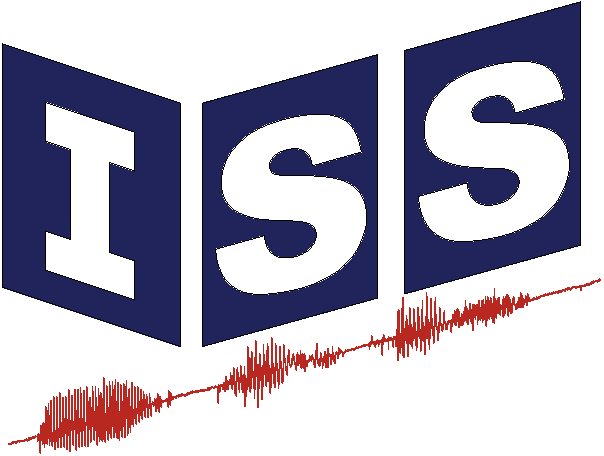
\includegraphics[width=28mm]{isslogocolor}
}
\subject{\worksubject\vspace*{-5mm}} % Art und Nummer der Arbeit
\title{\maintitle}%\\ \Large{\subtitle}}
\subtitle{\translatedtitle}
\author{
\large
  \ifthenelse{\equal{\doclang}{german}}{
  \begin{tabular}{rp{7cm}}
    \Large 
    Autor:      & \Large \student \vspace*{2mm}\\
    Ausgabe:    & \startdate \\
    Abgabe:     & \submission \vspace*{3mm}\\
    Betreuer:   & \tutor \vspace*{2mm}\\
    Stichworte: & \keywords
  \end{tabular}
  }{
  \begin{tabular}{rp{7cm}}
    \Large 
    Author:             & \Large \student \vspace*{2mm}\\
    Date of work begin: & \startdate \\
    Date of submission: & \submission \vspace*{3mm}\\
    Supervisor:         & \tutor \vspace*{2mm}\\
    Keywords:           & \keywords
  \end{tabular}
  }
  \bugfix
}
\date{}
\publishers{\normalsize
  \begin{minipage}[t]{.9\textwidth}
    \abstract
  \end{minipage}
}

\numberwithin{equation}{chapter} 
\sloppy 

%
%
%
% *****************************************************************
% --------------> put typography definitions here <----------------
% *****************************************************************
% colors
\definecolor{darkblue}{rgb}{0,0,0.4}

% declarations
\newcommand{\matlab}{\textsc{Matlab}\raisebox{1ex}{\tiny{\textregistered}} }
% Integers, natural, real and complex numbers
\newcommand{\Z}{\mathbb{Z}}
\newcommand{\N}{\mathbb{N}}
\newcommand{\R}{\mathbb{R}}
\newcommand{\C}{\mathbb{C}}
% expectation operator
\newcommand{\E}{\operatorname{E}}
% imaginary unit
\newcommand{\im}{\operatorname{j}}
% Euler's number with exponent as parameter, e.g. \e{\im\omega}
\newcommand{\e}[1]{\operatorname{e}^{\,#1}}
% short command for \operatorname{}
\newcommand{\op}[1]{\operatorname{#1}}

% unknown hyphenation rules
\hyphenation{Im-puls-ant-wort Im-puls-ant-wort-ko-ef-fi-zien-ten
Pro-gramm-aus-schnitt Mi-kro-fon-sig-nal}
% *****************************************************************
%
\makeglossaries

\newabbreviation{adc}{ADC}{Analog-to-digital conversion}
\newabbreviation{amr}{AMR}{Autonomous mobile robot}
\newabbreviation{aoa}{AoA}{Angle of arrival}
\newabbreviation{aod}{AoD}{Angle of departure}

\newabbreviation{ble}{BLE}{Bluetooth low-energy}

\newabbreviation{ca}{CA}{Cell averaging}
\newabbreviation{cfar}{CFAR}{Constant false alarm rate}
\newabbreviation{cir}{CIR}{Channel impulse response}
\newabbreviation{cri}{CRI}{Chirp repetition interval}
\newabbreviation{cs}{CS}{Chirp sequence}
\newabbreviation{cut}{CUT}{Cell under test}

\newabbreviation{dsp}{DSP}{Digital signal processor}

\newabbreviation{e-field}{E-field}{Electric field}

\newabbreviation{fft}{FFT}{Fast Fourier transform}
\newabbreviation{fm}{FM}{Frequency modulated}
\newabbreviation{fmcw}{FMCW}{Frequency modulated continuous wave}

\newabbreviation{gltf}{glTF}{GL transmission format}
\newabbreviation{gps}{GPS}{Global positioning system}

\newabbreviation{hpbw}{HPBW}{Half power beam width}
\newabbreviation{h-field}{H-field}{Magnetic field}

\newabbreviation{if signal}{IF signal}{Intermediate frequency signal}
\newabbreviation{ior}{IOR}{Index of refraction}

\newabbreviation{los}{LOS}{Line of sight}
\newabbreviation{lpf}{LPF}{Low-pass filtering}
\newabbreviation{lrp}{LRP}{Local reference point}

% \newabbreviation{maxnumreflections}{MaxNumReflections}{Maximum number of the reflections}
% \newabbreviation{maxnumdiffractions}{MaxNumDiffractions}{Maximum number of the diffractions}
% \newabbreviation{maxrelativepathloss}{MaxRelativePathLoss}{Maximal relative path loss}
% \newabbreviation{maxabsolutepathloss}{MaxAbsolutePathLoss}{Maximal absolute path loss}
\newabbreviation{mimo}{MIMO}{Multiple input, multiple output}
\newabbreviation{mom}{MoM}{Method of moments}

\newabbreviation{nlos}{NLOS}{Non-line-of-sight}

\newabbreviation{pdf}{PDF}{Probability density function}

\newabbreviation{rcs}{RCS}{Radar cross-section}
\newabbreviation{rd map}{RD map}{Range-Doppler map}
\newabbreviation{rssi}{RSSI}{Receive signal strength indication}
\newabbreviation{rx}{RX}{Receiver}

\newabbreviation{sbr}{SBR}{Shooting and bouncing ray}
\newabbreviation{snr}{SNR}{Signal-to-noise ratio}

\newabbreviation{tx}{TX}{Transmitter}

\newabbreviation{uwb}{UWB}{Ultra-wideband}

\begin{document}

% title and table of contents
\pagenumbering{alph}
\maketitle
\cleardoublepage
\pagenumbering{roman} % roman numbering for table of contents
\tableofcontents
\cleardoublepage
\renewcommand{\glossarypreamble}{\glsfindwidesttoplevelname[\currentglossary]}
\setglossarystyle{alttree}
% \printglossaries
\printunsrtglossary[type=abbreviations]
\cleardoublepage
\noindent
\begin{minipage}[t]{\textwidth}
    \chapter*{Abstract}
    \addcontentsline{toc}{chapter}{Abstract}
    With the emerging interest in indoor positioning, our goal is to build a millimeter wave indoor localization system based on the active radar sensing of local passive reference points which reduces costs but ensures its accuracy. However, building a real system is time-consuming and expensive, so this thesis is aiming at building a ray tracing channel simulation to easily calculate the channel impulse response (CIR) and received signal by the radar system. Meanwhile, in order to make the scene closer to the real world, we will build a larger and more complicated room model in Blender, then simulate and apply the raytracing including the anisotropic antenna radiation pattern and radar cross-section (RCS) in Matlab. Further, range-Doppler maps of the simulated baseband receive signal at different points along a moving robots trajectory are evaluated. Constant false alarm rate (CFAR) target detection is carried out and the plausibility of our simulation results is verified. The novel approach shows the range and velocity of the robot related to the targets in CFAR plot accurately and stabily.
\end{minipage}%
\hfill
\begin{minipage}[t]{\textwidth}
    \chapter*{Kurzfassung}
    % \addcontentsline{toc}{chapter}{Kurzfassung}
    Angesichts des wachsenden Interesses an der Innenraumortung ist es unser Ziel, ein Millimeterwellen-Innenraumlokalisierungssystem zu bauen, das auf der aktiven Radarerfassung lokaler passiver Referenzpunkte basiert, was die Kosten senkt, aber gleichzeitig die Genauigkeit gewährleistet. Der Aufbau eines realen Systems ist jedoch zeitaufwändig und teuer, daher zielt diese Arbeit darauf ab, eine Raytracing-Kanalsimulation zu erstellen, um die Kanalimpulsantwort (CIR) und das vom Radarsystem empfangene Signal einfach berechnen zu können. Um die Szene der realen Welt näher zu bringen, werden wir ein größeres und komplizierteres Raummodell in Blender erstellen und dann das Raytracing einschließlich des anisotropen Antennenstrahlungsmusters und des Radarquerschnitts (RCS) in Matlab simulieren und anwenden. Darüber hinaus werden Entfernungs-Doppler-Karten des simulierten Basisband-Empfangssignals an verschiedenen Punkten entlang der Flugbahn eines sich bewegenden Roboters ausgewertet. Es wird eine Zielerkennung mit konstanter Falschalarmrate (CFAR) durchgeführt und die Plausibilität unserer Simulationsergebnisse überprüft. Der neuartige Ansatz zeigt die Reichweite und Geschwindigkeit des Roboters in Bezug auf die Zielpunkte im CFAR-Diagramm genau und stabil.
\end{minipage}

\cleardoublepage
\setcounter{page}{1}
\pagenumbering{arabic} % arabic numbering for rest of document

% *****************************************************************
% -------------------> start writing here <------------------------

\chapter{Introduction} \label{introduction}
In recent years, with the development of automation technology and increasing amounts of various applications, the autonomous mobile robot (AMR) has been used widely in many areas \cite{usage_AMR}. In factories, there are some robots that can move with the help of high-speed networks and tracks or specified routes. However, the AMR need to complete tasks in more complex environments without tracks or specified path. For AMR to better complete their work, a reliable and accurate localization system for the indoor scenery becomes more important. The goal of this thesis is to develop a toolchain to calculate the channel impulse response (CIR) and radar receive signal for an AMR with a given position and velocity in an indoor environment using ray tracing channel simulation. The expected effect should be that the LRPs are clearly visible in the range-Doppler map and constant false alarm rate (CFAR) detection and can be accurately matched with the known range and velocity information. Meanwhile, it can be tested whether changes in multiple parameters will affect the accuracy and stability.

In this chapter, we will introduce the reasons for choosing a millimeter-wave localization system based on active radar sensing of local passive reference points (LRP) and simulating the system with ray tracing in Matlab, the goals of this thesis, and the structure of the entire thesis.

\begin{spacing}{1.5}
\textbf{\large{Millimeter wave localization system}}
\end{spacing}

For outdoor localization, there are already mature and accurate satellite positioning methods, such as GPS. However, there is no unified solution for indoor positioning, because different methods and hardwares have their advantages and disadvantages. Common methods include fingerprinting, low-energy Bluetooth (BLE), ultra-wideband (UWB), and so on \cite{methods_indoor_positioning}.

The fingerprinting method \cite{fingerprinting} refers to collecting unique signal features and corresponding location information at any specific location, comparing the signal collected by the receiver in real-time with the signal features in the database, and thus inferring the current location in the scene. These features include signal intensity, signal type, signal identifier, etc. Its advantage is that, for instance, if the indoor positioning is based on the WiFi fingerprinting, additional hardware is not required additionally, because most of the buildings have the WiFi equipment already. But the main disadvantage is that this method has the strong dependence on the environment, such as the moving people or the stationary objects. Moreover, building a database is also a huge task. If the system considers the intensity of the signals, the power density of the signal decreases with an increase in the distance, hence, the grid size of the room has a great impact on the accuracy of localization. However, as the resolution of the grid size increases, the cost and difficulty of the database will also rapidly increase.

The advantage of localization with low-power Bluetooth (BLE) \cite{cost_BLE} is that the equipment cost is relatively low and the power consumption is small. Meanwhile, it has been already installed on most electronic products such as mobile phones and smart home devices. The low-power Bluetooth currently uses two main methods. One is fingerprint positioning as mentioned above, and the other is multilateration. Both methods are based on the receive signal strength indication (RSSI). By analyzing the distances between the three points, the location of the object can be determined. However, according to \cite{BLE}, the accuracy estimation of the BLE system is usually roughly $1.5\,\mathrm{m}$. However, in the simulation scenario of this thesis, the edge size of the room is $20\,\mathrm{m}$. If the error of the range is $1.5\,\mathrm{m}$, the deviation of the position will appear large in this room, so this method is not suitable for the environment of this article.

The advantage of ultra-wideband localization \cite{UWB} is that it expands the bandwidth, effectively reducing interference from other objects and signals, and has good penetration ability, which has the characteristics of good robustness and improves adaptability to complex situations and positioning accuracy. However, due to the large number of reference nodes, calculating the propagation time of signals from these points separately and synchronizing them throughout the system will make the entire system complex and costly.

Therefore, considering the advantages and disadvantages of the above methods, we chose to use the millimeter wave indoor localization system based on active radar sensing of local passive reference points \cite{schlachter_indoor_2024}, the Figure \ref{conceptual view} demonstrates the conceptual view of the system. It can reduce the system cost, and developing the radar system using a single transmitter and a single receiver on the robot can also achieve a high accuracy. For this system, we choose a radar called frequency modulated continuous wave (FMCW) radar, which can actively transmit signals and the signals will be reflected when passing through walls or other objects and then captured by the receiver. The local reference point (LRP) in this article can be understood as a target. By placing some targets in the room, which are hung on the ceiling or fixed at the corner of the room, and then observing the effect of these target points in the signal processing. In this thesis, reflectors are used as local reference points. There are two types of reflectors, one is called the trihedral corner reflector and the other one is called the octahedral reflector. Meanwhile, building a real system is a time-consuming task, so the radar system in this thesis will use raytracing channel simulation methods to offer high realism and simple application of the channel simulation method to a vast spectrum of test scenarios.

\begin{figure}
	\centering
	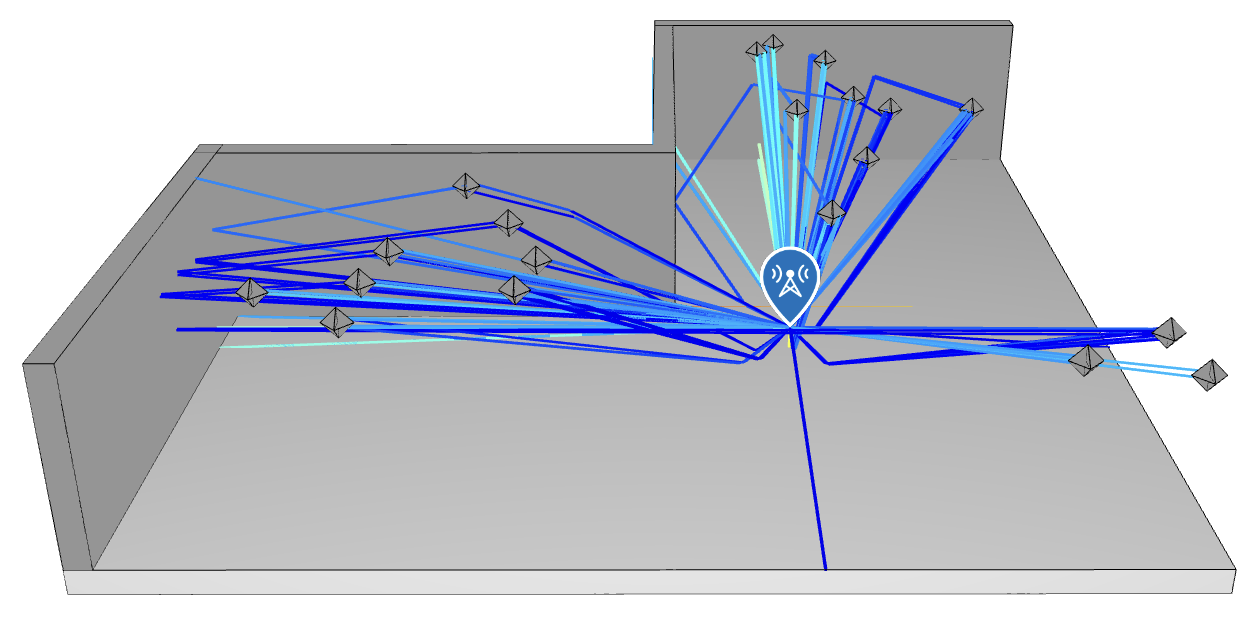
\includegraphics[scale=.4]{figures/thesis_plot.png}
	\caption{The conceptual view of the millimeter wave indoor localization system}
	\label{conceptual view}
\end{figure}

\begin{spacing}{1.5}
\textbf{\large{Ray tracing}}
\end{spacing}

As an illumination method, ray tracing can more realistically simulate optical phenomena such as reflection and diffraction with the advancement of computer graphics \cite{raytracing_introduction}. In this thesis, we use the ray tracing offered in Matlab to simulate the propagation process of millimeter waves and get the propagation properties, such as path loss, propagation distance, angle, and other parameters.

The wavelength of visible light is usually between 400 nanometers and 700 nanometers, while the wavelength of millimeter waves is usually between 1 millimeter and 10 millimeters. Ray tracing is used to simulate the propagation process of millimeter waves mainly because the millimeter waves behave similarly to light. Compared with the light, millimeter waves propagate in a straight line in free space as well, which means that ray tracing methods can be used to obtain the propagation distance. Millimeter waves also have characteristics such as reflection, diffraction, scattering, and so on, and follow the same laws such as the law of reflection as in the optical field. Then, various losses will also occur during the propagation process. These attenuation characteristics are very similar to the propagation behavior of light in the medium, so ray tracing can also be used to simulate millimeter-wave and analyze the loss information.

\begin{spacing}{1.5}
\textbf{\large{Structure of thesis}}
\end{spacing}

The thesis mainly consists of the following four parts: radar signal modeling, ray tracing channel simulation, signal processing and evaluation, summary and outlook.

Radar signal modeling mainly focuses on the radar system itself, by demonstrating the principles and foundations of the radar system and the selection of parameters, thus setting up the foundations of the toolchain, namely in Chapter \ref{Radar signal modeling}.

The ray tracing channel simulation includes the modeling of the room, the simulation of ray tracing in the room, applying the anisotropic radiation pattern of the antenna, the simulation of the anisotropic RCS pattern, and the generation of the robot's continuous motion process, which is shown in Chapter \ref{Ray tracing channel simulation}.

Radar signal processing will use the properties of received rays and the formulas introduced in Chapter \ref{Radar signal modeling} to process the data from Chapter \ref{Ray tracing channel simulation}. The processed data will be displayed through two methods, namely range-Doppler map and CFAR detection which will be introduced in Section \ref{Range-Doppler map} and Section \ref{CFAR detection} respectively. Then, Section \ref{Evaluation} will show the results as well as evaluate the influence of various parameters and settings, checking whether the expected effect is achieved as mentioned above, and analyzing the rationality of various parameters. Finally, Chapter \ref{Summary and outlook} "Summary and Outlook" summarizes this thesis and analyzes what could be further improved in the future research.


\chapter{Radar signal modeling} \label{Radar signal modeling}
This chapter mainly contains five sections. Section \ref{Radar foundation} and section \ref{FMCW radar} introduce the principles and foundations of the radar system; Section \ref{Radar system parameters} is about the selection of default parameters in the radar system; Section \ref{Radar range equation} will introduce the radar range equation and calculate the path loss to obtain the minimum required radar power under the condition of the targeted signal-to-noise ratio (SNR) value; Section \ref{Signal model} will introduce the formula of the baseband receive signal for subsequent signal processing.

\section{Radar foundation} \label{Radar foundation}
The signal flow in this thesis is shown in Figure \ref{signal_flow}, which demonstrates the signal transmission in the case of a single chirp and processing by the model. $s(t)$ represents the transmitted chirp. After being transmitted through the antenna TX, it will be captured by the RX after reflections, diffractions and the propagation distance which result in the attenuation and delay. $h(t)$ means the impulse response of a target, which represents the delay and attenuation above. Therefore, the obtained signal has a similar frequency slope but a lag effect compared to the transmitted signal. After mixing the transmitted and received signals, the new signal is called the beat signal \cite{beat_frequence_signal}, whose frequency is the absolute value of the difference between those two signal frequencies. Therefore, the frequency of the beat signal is proportional to the delay or propagation distance, which is explained in detail in section \ref{FMCW radar}. The final signal $x(t)$ is called low frequency baseband signal. In this thesis we will model this signal for multiple chirps rather than a single chirp.

\begin{figure}
	\centering
	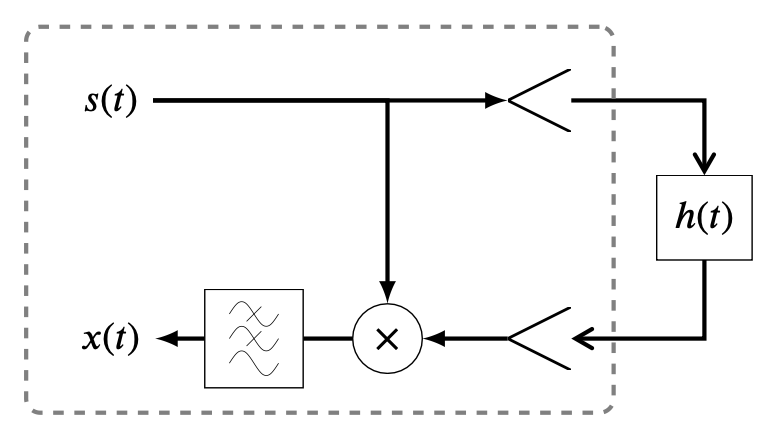
\includegraphics[scale=.6]{figures/signal_flow.png}
	\caption{The signal flow \cite{hafner_parameter_2021}}
	\label{signal_flow}
\end{figure}

\begin{spacing}{1.5}
\textbf{\large{Range}}
\end{spacing}

The propagation distance usually refers to the length of the path that the signal travels from the transmitter to the receiver after reflections and diffractions at the target points. The distance value is proportional to the delay, and the coefficient is the speed of light. In the raytracing simulation, the range is estimated by the delay of a ray from TX to RX antennas which are quasi-monostatic, i.e. almost in the same position. However, the range what shows in the RD maps is the distance between the AMR and the target. Therefore, the range r between the robot and the target in this thesis should be proportional to half of the propagation delay, as shown in formula \ref{propagation delay formula},
\begin{equation}
    \centering
    r = c \cdot \frac{\tau}{2},
    \label{propagation delay formula}
\end{equation}
where $c$ represents the speed of light, namely $3 \times 10^8$ m/s, and $\tau$ represents the propagation delay.

\begin{spacing}{1.5}
\textbf{\large{Doppler effect}}
\end{spacing}

The Doppler Effect refers to the phenomenon of wave frequency change caused by the relative motion between a wave source and an observer. When the wave source and observer move closer, the frequency of the waves received by the observer increases; whereas, when they move away from each other, the frequency decreases. Since the reflector’s position is fixed while the robot is moving, the relative motion between them will generate the Doppler effect. The frequency of the received signal in the Doppler effect is
\begin{equation}
    \centering
    f' = f \left( \frac{c \pm v_o}{c \mp v_s} \right),
    \label{doppler shift formula}
\end{equation}
where $v_0$ and $v_s$ represent the relative velocity of the antenna as the source and target to the medium respectively. In the case of the radar system which the reflectors are stationary and the AMR moves, since both RX and TX are co-located on the AMR, the signal is Doppler shifted once from transmitter to the reflector, and then again from the reflector to receiver, that is, twice shifted. the frequency shift $f_d$ can be written as
\begin{equation}
    \centering
    f_d = \frac{2v \cos \theta}{\lambda} = \frac{2v\textsubscript{k}}{\lambda},
    \label{frequency shift formula}
\end{equation}
where $\theta$ represents the angle between the incident ray and the robot's velocity, i.e. $v_k$ represents the projection of the velocity on the incident ray. Figure \ref{the projection of the velocity} illustrates the projection.

\begin{figure}
	\centering
	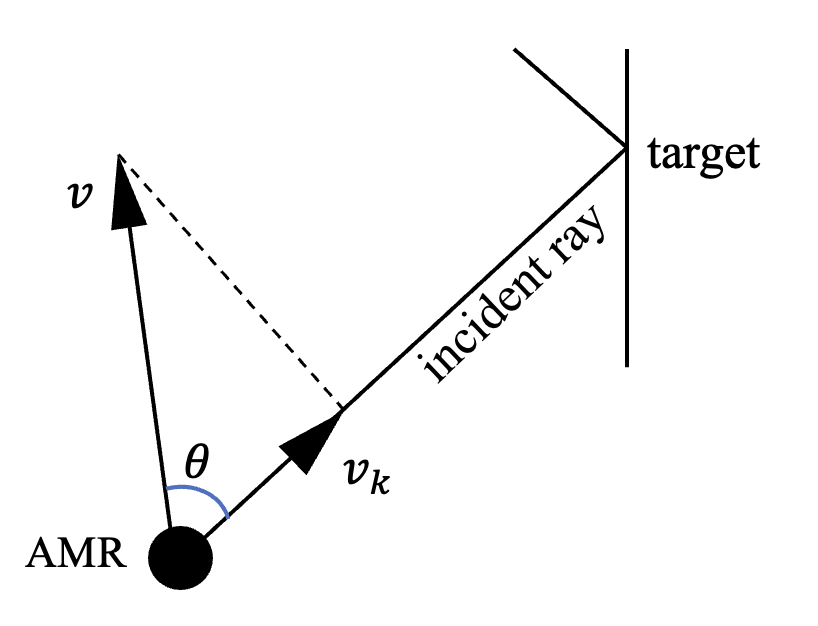
\includegraphics[scale=.4]{figures/velocity_AMR.png}
	\caption{The projection of the velocity}
	\label{the projection of the velocity}
\end{figure}

\begin{spacing}{1.5}
\textbf{\large{Radar cross-section}}
\end{spacing}

The radar cross-section (RCS) is a physical quantity that measures the intensity of the reflected rays by a target when illuminated by radar waves. It represents the hypothetical area of the target, expressed as the projected area of an equivalent isotropic reflector that produces the same echo power per unit angle in the receiving direction as the defined target \cite{rcs}. The radar cross-section is generally denoted as the symbol $\sigma$. The RCS depends on the shape, size, structure, and material of the target, as well as the frequency, polarization, and angle of incidence of the electromagnetic waves. In this article, we investigate different types of the reflector, such as trihedral corner reflector and octahedral reflector. The RCS peak value differs in different types of reflectors. For instance, the max formula of the triangular corner reflector \cite{doerry_reflectors_2014} is denoted as
\begin{equation}
    \centering
    \sigma = \frac{4 \pi a^{4}}{3 \lambda^{2}},
    \label{radar cross-section formula}
\end{equation}
where
\begin{enumerate}[label=\textbullet]
    \item a denotes the edge length of the trihedral corner reflector.
    \item $\lambda$ denotes the wavelength.
    \item The unit of $\sigma$ is m\textsuperscript{2}, which is same as the unit of area.
\end{enumerate}
For the real trihedral corner reflector, the RCS value will change as the angle changes, and the peak value occurs when the incident ray is perpendicular to each side while the max value occurs at bore-sight angle which will be introduced later. This formula will be calculated by hand in section \ref{Radar range equation}, and simulated the anisotropic pattern in section \ref{Reflector radar cross section}.

\begin{spacing}{1.5}
\textbf{\large{Path loss}}
\end{spacing}

There are many types of signal loss during transmission, including path loss, large-scale loss, and small-scale loss. In the raytracing of Matlab, the propagation loss for rays that are reflected from walls could be well simulated. While for line-of-sight (LOS) rays reflected between antenna and reflectors, the RCS of reflectors will be considered later, the physical reflection and scattering effects is already contained in the target RCS pattern, we choose to manually calculate the loss of these rays. The calculation formula for loss of the LOS ray \cite{path_loss} is as follows:
\begin{equation}
    \centering
    PL = 10\cdot\log_{10}\left(\frac{G_{T}G_{R}\lambda_{c}^{2}\cdot\sigma}{(4\pi)^{3} r^{4}}\right),
    \label{path loss formula}
\end{equation}
where
\begin{enumerate}[label=\textbullet]
    \item $G_T$ and $G_R$ are the gain value of transmitter and receiver respectively.
    \item $\lambda$ is the wavelength of the ray and can be calculated by $\lambda=c/f$.
    \item $\sigma$ is the radar cross-section as mentioned above.
    \item $r$ represents the propagation distance of LOS rays.
\end{enumerate}

\begin{spacing}{1.5}
\textbf{\large{Thermal noise}}
\end{spacing}

There are many types of noise in the radar system, the thermal noise is an important type among them, also known as Johnson-Nyquist noise \cite{richards_principles_2010} or white noise. Johnson-Nyquist noise exists in all electronic devices and transmission media, cannot be eliminated, and is dependent on the temperature. The formula is written as
\begin{equation}
    \centering
    N_{T} = k \cdot T_{S} \cdot \Delta f = k \cdot T_{S} \cdot \Delta f_s,
    \label{thermal noise formula}
\end{equation}
where
\begin{enumerate}[label=\textbullet]
    \item $k$ is Boltzmann's constant, namely $1.38 \times 10^{-23}$ watt-sec/K.
    \item $T_0$ is the standard temperature as 290 K.
    \item $F$ is the noise figure assumed as 1.
    \item $\Delta f$ represents the bandwidth of the baseband receive signal which should be its sampling frequency $f_s$.
\end{enumerate}

\begin{spacing}{1.5}
\textbf{\large{Polarization}}
\end{spacing}

The polarization of an antenna defines the direction of the electric field (E-field) and the magnetic field (H-field) of the electromagnetic waves that the antenna radiates or receives. The electric field (E-field) is a vector field that describes the electric force around the electric charge which has the same direction as the polarity of the antenna. The magnetic field (H-field) is a vector field that describes the magnetic force. It defines the direction and strength of the magnetic force at each point which is perpendicular to the direction of the E-field. Additionally, both the E-field and the H-field are perpendicular to the direction of signal propagation.

\begin{spacing}{1.5}
\textbf{\large{Microstrip antenna and radiation pattern}}
\end{spacing}

With the development of the microwave integration technology and new manufacturing processes, microstrip antennas have advanced. Compared to traditional antennas, microstrip antennas have many advantages, such as smaller size, lighter weight, easier integration, and lower cost. The structure of a microstrip antenna typically consists of a dielectric substrate, a radiating element, and a ground plane \cite{patchMicrostrip}. The thickness of the dielectric substrate is much smaller than the wavelength. The bottom of the substrate has a thin metal layer connected to the ground plane, while the front side is fabricated with a metal layer of specific shapes using photolithography to serve as the radiating element. The shape of the radiating patch can be varied according to requirements. And the microstrip antenna is able to be used in FMCW radar system.

Therefore, when designing a microstrip antenna, in addition to parameters such as length, width, and height, many other parameters can also be adjusted to achieve the desired maximum gain and radiation intensity in different directions. These parameters include the substrate thickness, the length and width of the ground plane, the position of the antenna radiating patch, the offset of the feed point, various parameters related to the conductors, and so on.

The radiation pattern is an important property of the antenna. It is useful for analyzing whether the antenna’s gain and coverage in various directions meet the requirements. Additionally, because the height of the robot is relatively much lower compared to the reflectors, we aim for the antenna signal strength to be concentrated primarily upwards rather than surroundings, which will be demonstrated in section \ref{Antenna radiation pattern}. This configuration better meets the realistic and complex simulation environment. Therefore, the gain $G$ of the antenna can be expressed in terms of efficiency and directivity as the following equation,

\begin{equation}
    \centering
    G = e \times D,
    \label{antenna gain formula}
\end{equation}

where $e$ represents the efficiency which is the ratio of power radiated by antenna to the input power and $D$ means the directivity which measures how focused the radiation pattern in the particular direction. Both variable are in the linear scale.

\section{FMCW radar} \label{FMCW radar}
Frequency-modulated continuous wave (FMCW) radar systems \cite{hafner_parameter_2021} are used in various fields nowadays, such as automotive radar, drone radar, and so on. The chirp frequency used in FMCW radar increases linearly with time, where this type of signal is known as linear frequency modulated (FM) signal. The left side of Figure \ref{FMCW_signal} illustrates the amplitude variation of a linear FM pulse chirp over time. The signal frequency will increase from the initial value $f_c$ by the amplitude of bandwidth $B$ during one chirp of duration $T_c$.

Continuous wave emphasizes that the radar transmits the single chirp continuously, rather than the pulse signals. However, there is usually a gap between the chirps, otherwise, aliasing will occur when processing the signal, affecting the accuracy of the result, i.e. the length of the repetition interval $T_p$ is usually larger than the length of the chirp duration $T_c$. The right one of Figure \ref{FMCW_signal} illustrates this transmission process and the linear frequency increase.

As previously mentioned, the beat frequency can be better understood in this context. The beat signal here can also be called the intermediate frequency (IF) signal, both indicating the difference frequency signal obtained by the ideal mixer after mixing the received signal with the transmitted signal. The frequency of the resulting beat signal is proportional to the time delay between the two signals. Figure \ref{IF_signal} illustrates this process well.

\begin{figure}
    \centering
    \hspace{-0.4cm}
    \begin{subfigure}{0.45\textwidth}
        \centering
        \adjustbox{height=5cm}{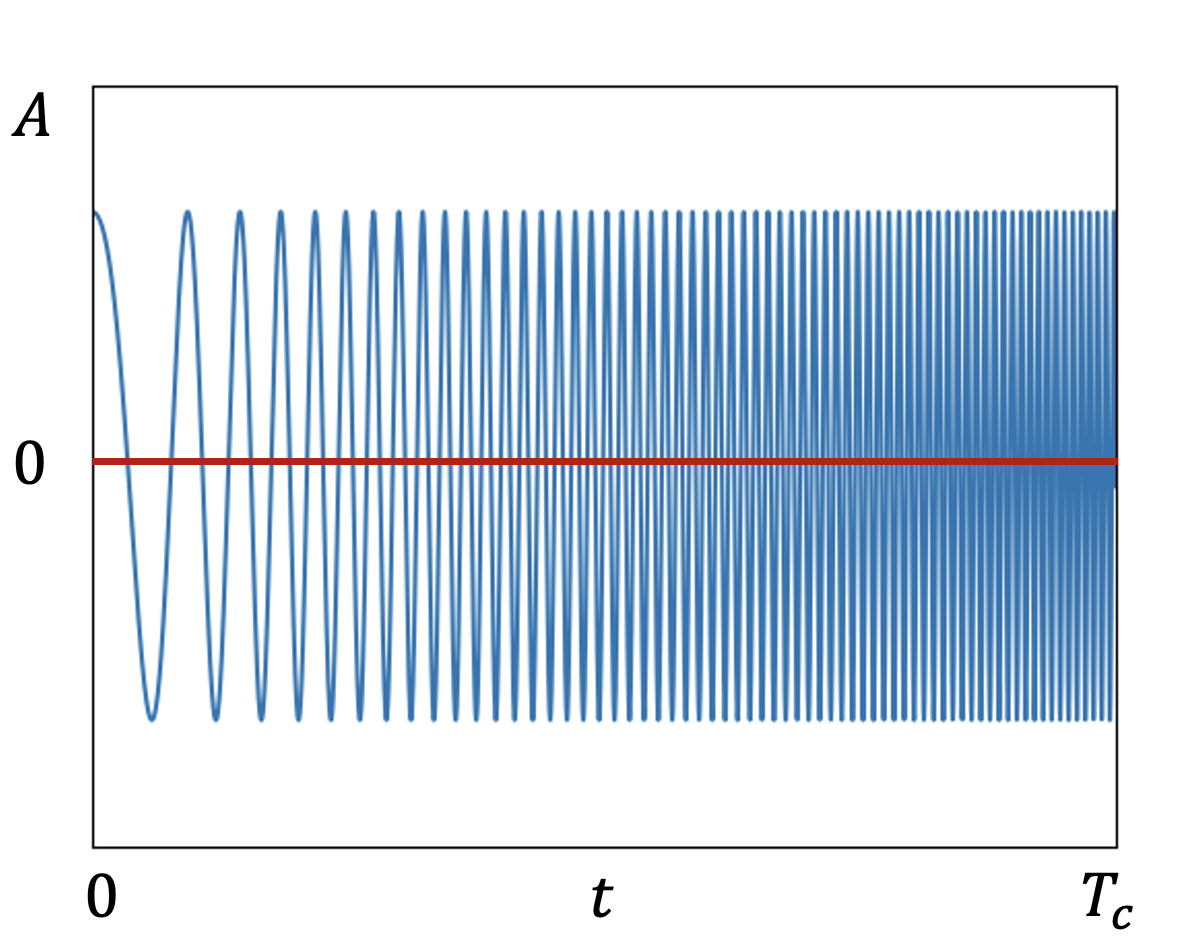
\includegraphics[scale=.3]{figures/FMCW_signal_left.png}}
    \end{subfigure}
    \begin{subfigure}{0.45\textwidth}
        \centering
        \adjustbox{height=5cm}{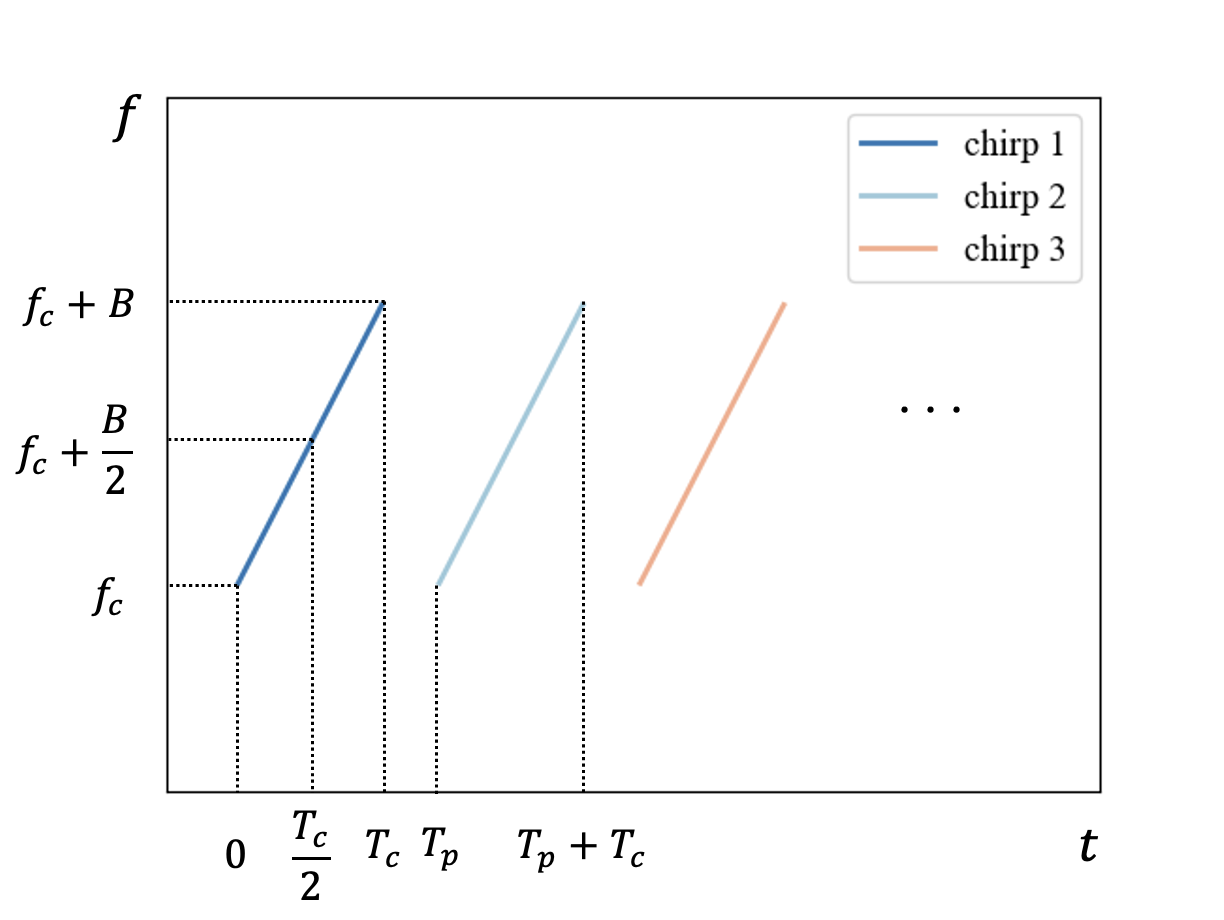
\includegraphics[scale=.3]{figures/FMCW_signal_right.png}}
    \end{subfigure}
    \caption{The amplitude and frequency variation of FMCW radar in time respectively}
	\label{FMCW_signal}
\end{figure}

\begin{figure}
    \centering
    \begin{subfigure}{0.45\textwidth}
        \centering
        \adjustbox{height=5cm}{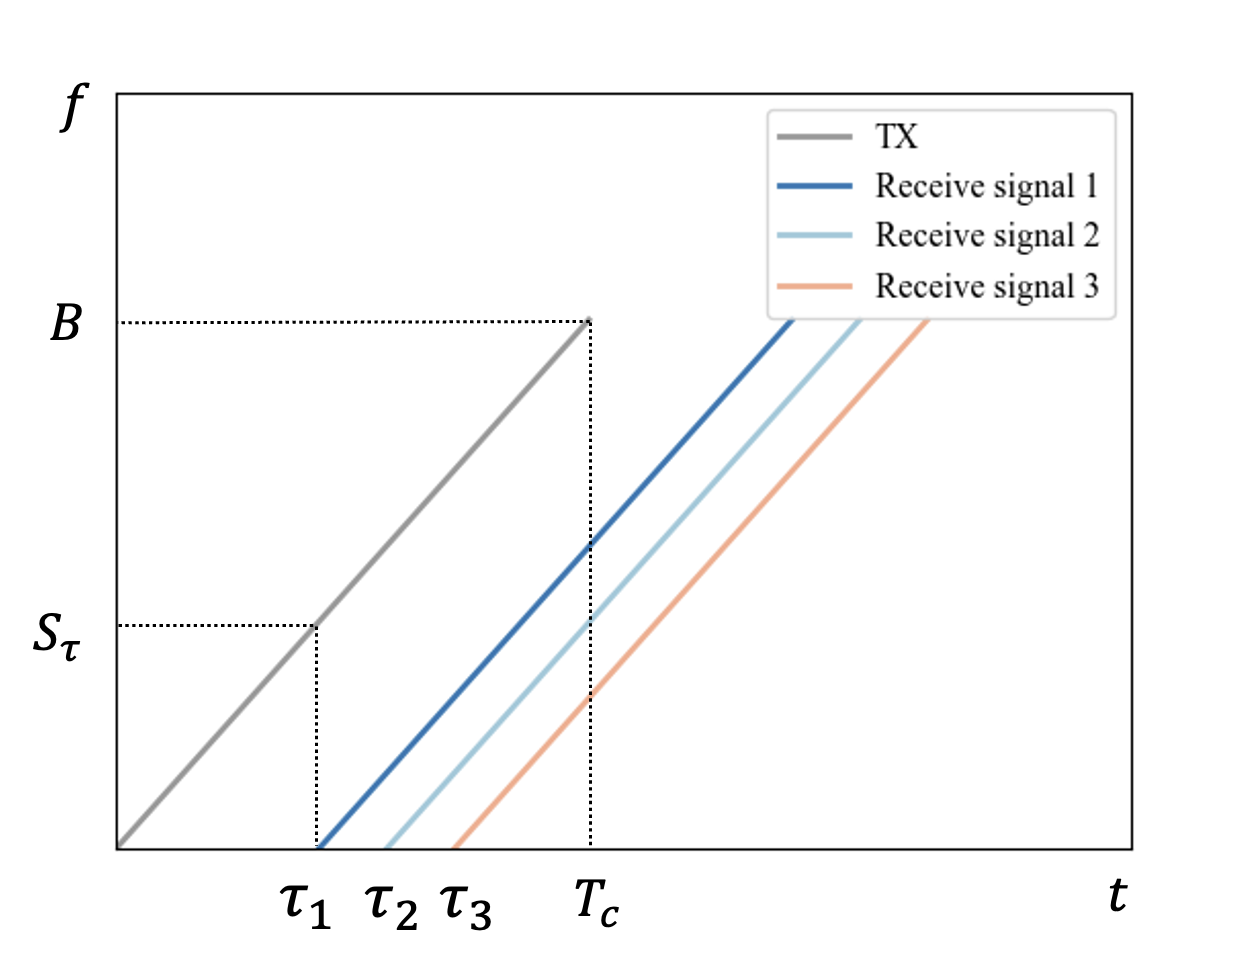
\includegraphics[scale=.3]{figures/IF_signal_left.png}}
    \end{subfigure}
    \begin{subfigure}{0.45\textwidth}
        \centering
        \adjustbox{height=5cm}{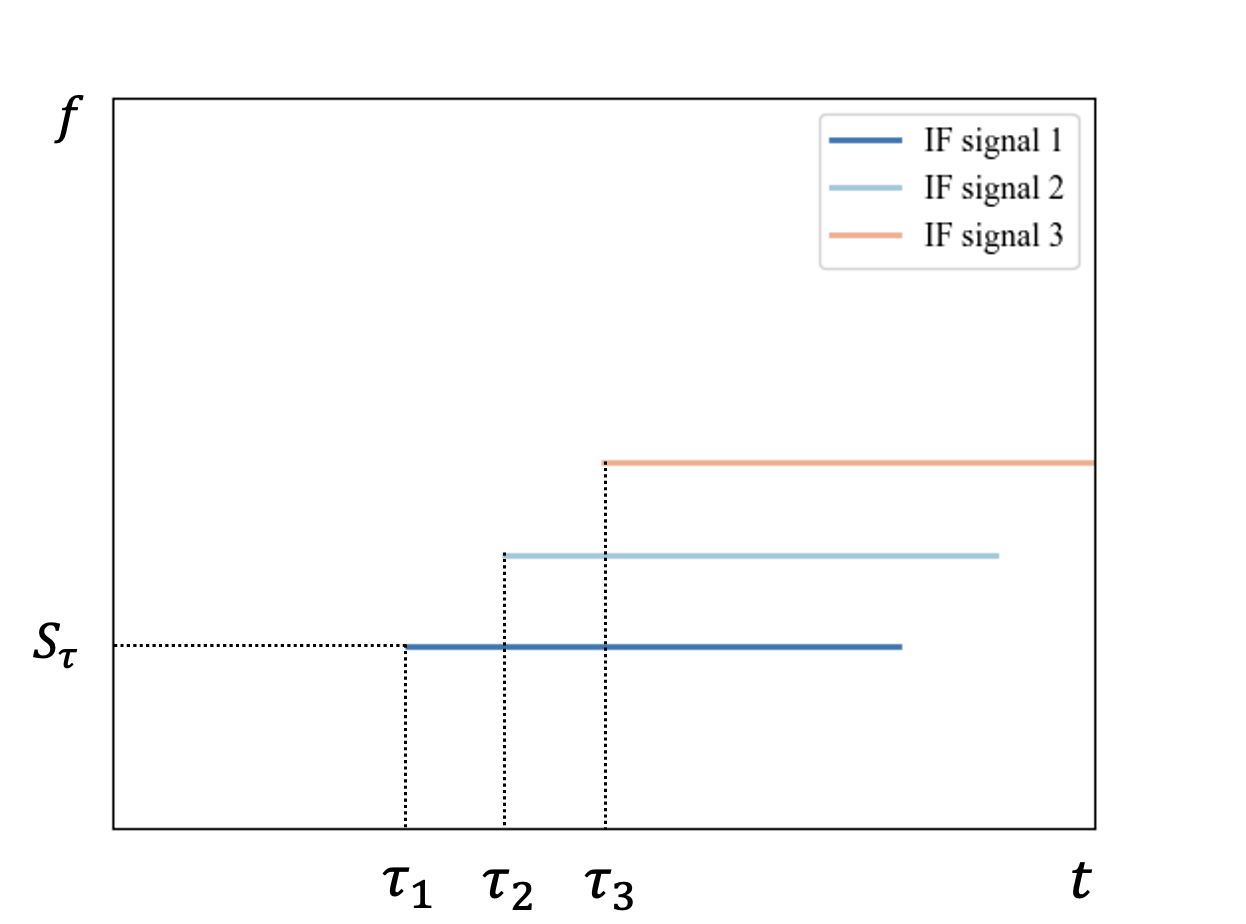
\includegraphics[scale=.3]{figures/IF_signal_right.png}}
    \end{subfigure}
    \caption{Intermediate frequency (IF) signal}
	\label{IF_signal}
\end{figure}

Therefore, a signal includes multiple chirps, each chirp is continuous, and there are intervals between chirps. A chirp contains the initial frequency ($f_c$), bandwidth ($B$), and duration ($T_c$). The slope ($S$) of the chirp represents the rate of increase of the frequency in time, namely $S=B/T_c$. $S_{\tau}$ is the frequency difference corresponding to the delay time $\tau$.

\begin{spacing}{1.5}
\textbf{\large{Range resolution}}
\end{spacing}

Range resolution is the ability to distinguish between two or more objects. When two objects are very close to each other, the signals in the frequency domain processed after a Fourier transform may become hard to distinguish. To solve this problem, it is necessary to improve the range resolution, which requires the large bandwidth. As the Rayleigh criterion shown in Figure \ref{range_resolution}, as the chirp transmission duration increases, the length of the intermediate frequency (IF) signal increases, and the corresponding bandwidth also increases. This results in more peaks in the frequency domain, allowing for better distinction between objects.

\begin{figure}[t]
	\centering
	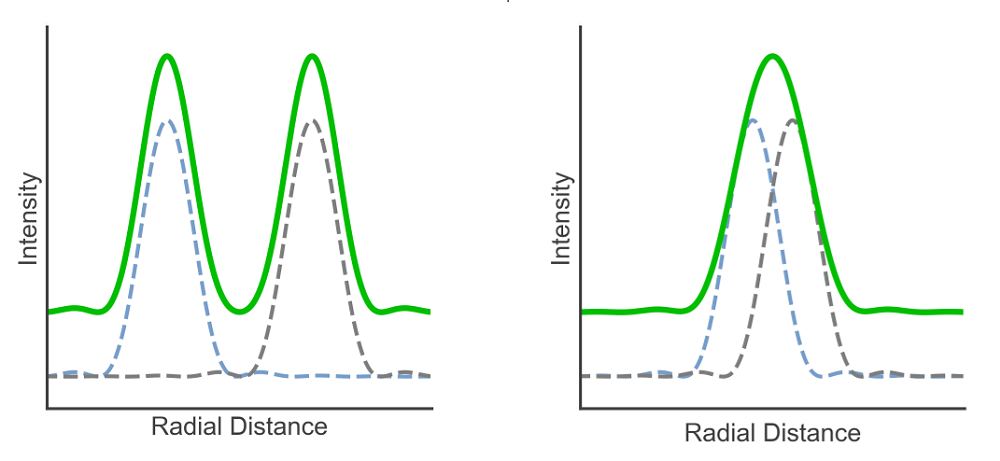
\includegraphics[scale=.5]{figures/rayleigh_criterion.png}
	\caption{The conceptual view of the Rayleigh criterion \cite{granite_rayleigh_nodate}}
	\label{range_resolution}
\end{figure}

When the distance between the reflector and the robot is $r$, the frequency of the intermediate frequency signal generated is
\begin{equation}
    \centering
    f = S\cdot\frac{2r}{c},
\end{equation}
therefore, if the distance between the two objects is $\Delta r$, the frequency difference for the intermediate frequency signal is
\begin{equation}
    \centering
    \Delta S_\tau = \Delta f = S\cdot\frac{2\Delta r}{c}.
\end{equation}
Since the duration of a chirp is $T_c$, the intermediate frequency difference should satisfy:
\begin{equation}
    \centering
    S\cdot\frac{2\Delta r}{c} \geq \frac{1}{T\textsubscript{c}}.
    \label{intermediate frequency difference formula}
\end{equation}
According to the definition of chirp slope above,
\begin{equation}
    \centering
    B = S \cdot T\textsubscript{c}.
\end{equation}
Therefore, the condition that the range resolution of the radar system must satisfy is:
\begin{equation}
    \centering
    \Delta r \geq \frac{c}{2B}.
    \label{range resolution formula}
\end{equation}

\begin{spacing}{1.5}
\textbf{\large{Maximum range}}
\end{spacing}

According to formula \ref{intermediate frequency difference formula}, the maximum frequency of intermediate frequency (IF) signal $f\textsubscript{IF\_max}$ can be deduced with the maximum range $r_{max}$,
\begin{equation}
    \centering
    f\textsubscript{IF\_max}\ = S \cdot \frac{2r\textsubscript{max}}{c}.
\end{equation}
The intermediate frequency (IF) signal typically needs to be digitized through low-pass filtering (LPF) and analog-to-digital conversion (ADC) to enable further processing on a digital signal processor (DSP). Therefore, the bandwidth of the IF signal is limited by the sampling frequency ($F_s$) of the ADC, namely
\begin{equation}
    \centering
    F\textsubscript{s} \geq S \cdot \frac{2r\textsubscript{max}}{c}.
\end{equation}
The sampling rate therefore limits the maximum range to
\begin{equation}
    \centering
    r\textsubscript{max} = \frac{F\textsubscript{s}c}{2S} = \frac{cN\textsubscript{s}}{2B},
    \label{maximum range formula}
\end{equation}
where $N_s$ refers to the number of sampling points collected in one chirp duration, written as
\begin{equation}
    \centering
    N\textsubscript{s} = F\textsubscript{s} \cdot T\textsubscript{c}.
    \label{sampling frequency formula}
\end{equation}

\begin{spacing}{1.5}
\textbf{\large{Velocity resolution}}
\end{spacing}

Similar to range resolution, the velocity of the robot causes Doppler shifts between different chirps. The velocity of the AMR is estimated by the Doppler shift, where the velocity resolution $\Delta v$ is the minimum speed difference that can be distinguished. This Doppler shift must also meet the minimum resolution requirement during the fast Fourier transform (FFT). The FFT frequency $f_{FFT}$ is related to the total sampling duration, which is determined by the number of chirps and the repetition interval. As the chirp interval increases, it becomes easier to observe speed difference in the frequency domain, thereby improving the velocity resolution, namely
\begin{equation}
    \centering
    f\textsubscript{FFT} = \frac{1}{T\textsubscript{p} N\textsubscript{p}},
\end{equation}
where $T_p$ means the repetition interval between chirps and $N_p$ represents the number of chirps. According to the frequency shift obtained from equation \ref{frequency shift formula} above, if the robot is moving, this frequency shift should be greater than or equal to the FFT resolution, i.e.
\begin{equation}
    \centering
    \frac{2v_k}{\lambda} \geq \frac{1}{T\textsubscript{p} N\textsubscript{p}}.
\end{equation}
Therefore, the minimum velocity can be written as
\begin{equation}
    \centering
    v_k \geq \frac{\lambda}{2} \cdot \frac{1}{T\textsubscript{p} N\textsubscript{p}} = \frac{c}{2f\textsubscript{c}} \cdot \frac{1}{T\textsubscript{p} N\textsubscript{p}},
\end{equation}
namely the velocity resolution along the direction of the incident ray that could be distinguished in FFT is
\begin{equation}
    \centering
    \Delta v_k = \frac{c}{2f\textsubscript{c}} \cdot \frac{1}{T\textsubscript{p} N\textsubscript{p}}.
    \label{velocity resolution formula}
\end{equation}

\begin{spacing}{1.5}
\textbf{\large{Maximum velocity}}
\end{spacing}

The maximum measurable velocity of an FMCW radar is typically limited by the repetition frequency of chirps, which determines the maximum frequency shift the radar can distinguish between two successive chirps. According to the Nyquist sampling theorem, the maximum measurable Doppler shift $f_{d \_ max}$ is half of the repetition frequency, namely
\begin{equation}
    \centering
    f\textsubscript{d\_max} = \frac{1}{2T\textsubscript{p}}.
    \label{maximum frequency shift formula}
\end{equation}
By inserting equation \ref{maximum frequency shift formula} into equation \ref{frequency shift formula}, the following expression for the maximum measurable velocity $v_{max}$ can be derived as
\begin{equation}
    \centering
    v\textsubscript{max} = \frac{f\textsubscript{d\_max} \cdot c}{2f\textsubscript{c}} = \frac{c}{4f\textsubscript{c} \cdot T\textsubscript{p}}.
    \label{maximum velocity formula}
\end{equation}
Combining equation \ref{velocity resolution formula} and equation \ref{maximum velocity formula}, the maximum velocity value in dependence on number of chirps can be derived as
\begin{equation}
    \centering
    v\textsubscript{max} = \frac{N\textsubscript{p}}{2} \cdot \Delta v\textsubscript{k}.
    \label{maximum velocity in dependence on number of chirps formula}
\end{equation}

\begin{spacing}{1.5}
\textbf{\large{Range migration}}
\end{spacing}

The measurement duration of the range-Doppler (RD) map refers to a complete period that includes multiple chirps. When a target point moves to different range cells between multiple chirp signals, the signal after processing will be dispersed among multiple range cells. Due to this dispersion, the signal-to-noise ratio (SNR) in each cell will decrease, given that the noise power remains constant. Therefore, the target point should be able to ensure falling within a single range cell.

To avoid the problem of range cell migration, the motion distance $d$ of the target between different chirps in one observation period should be less than half of the distance resolution, i.e.,
\begin{equation}
    \centering
    d \leq \frac{\Delta r}{2},
\end{equation}
where along the repetition interval in one measurement period the motion distance is
\begin{equation}
    \centering
    d = v \cdot T\textsubscript{r} \cdot N\textsubscript{c}.
\end{equation}
Combining both equations, the new inequality can be derived as
\begin{equation}
    \centering
    T\textsubscript{p} \cdot N\textsubscript{p} \leq \frac{\Delta r}{2v\textsubscript{max}}.
    \label{radar migration formula}
\end{equation}

\section{Radar system parameters} \label{Radar system parameters}
In this section, we will calculate the parameters of the radar system based on the environment simulated in this thesis, such as the size of the room, the parameters of the robot, and the desired resolution. A larger and more realistic room scene compared to \cite{schlachter_indoor_2024} is used in L-shaped.

The resolution of range and velocity will directly affect the accuracy of the target in the final range-Doppler map and CFAR detection. The range resolution would be chosen as
\begin{equation}
    \centering
    \Delta r\textsubscript{spec} = 0.1\,\mathrm{m},
\end{equation}
and the velocity resolution would be specified as
\begin{equation}
    \centering
    \Delta v\textsubscript{spec} = 0.5\,\mathrm{m/s}.
\end{equation}
Since the simulated room in this article is a larger and more realistic one with a size of $20 \,\mathrm{m} \times 20 \,\mathrm{m} \times 4 \,\mathrm{m}$, the maximum distance in the room is its diagonal path, i.e. $28.57\,\mathrm{m}$. However, a large detectable distance has high requirements on the radar's transmission power because the path loss related to the four power of the range increases a lot. Therefore, we will not consider targets that are too far away and set the maximum detection range firstly to
\begin{equation}
    \centering
    r\textsubscript{max} = 10\,\mathrm{m}.
\end{equation}
The velocity of an automatic mobile robot in default is usually below $2\,\mathrm{m/s}$. In order to leave a part of the velocity range that cannot be detected in CFAR, the maximum detection speed can be chosen as
\begin{equation}
    \centering
    |v\textsubscript{max}| = 5\,\mathrm{m/s}.
\end{equation}
In the FMCW radar system, the frequency of a single chirp increases in time. The value of the initial frequency in each chirp is chosen as
\begin{equation}
    \centering
    f\textsubscript{c} = 60\,\mathrm{GHz},
\end{equation}
the wavelength in this frequency will be
\begin{equation}
    \centering
    \lambda\textsubscript{c} = \frac{c}{f\textsubscript{c}} = 5\,\mathrm{mm}.
\end{equation}

\begin{spacing}{1.5}
\textbf{\large{Parameters calculation of radar system}}
\end{spacing}

\begin{enumerate}

    \item Bandwidth\\
    According to equation \ref{range resolution formula}, the minimum bandwidth is determined by the specified range resolution $\Delta r_{spec}$
    \begin{equation}
        \centering
        B \geq \frac{c}{2\Delta r\textsubscript{spec}} = \frac{3 \times 10\textsuperscript{8}\,\mathrm{m/s}}{2 \cdot 0.1\,\mathrm{m}} = 1.5\,\mathrm{GHz}.
    \end{equation}
    A larger bandwidth is beneficial to the improvement of range resolution, while a higher sampling rate will be also required on the radar system. Therefore, as a compromise, the bandwidth will be determined as $2\,\mathrm{GHz}$.
    
    \item Chirp repetition interval (CRI)\\
    According to formula \ref{maximum velocity formula}, the chirp repetition interval is limited by the maximum velocity. Considering that velocity as a vector has direction, although the maximum velocity value in different directions are not always the same, for calculating the limit of required parameters, we assume the maximum velocity value as $5\,\mathrm{m/s}$, and the repetition interval is calculated based on this, that is,
    \begin{equation}
        \centering
        T\textsubscript{p} \leq \frac{c}{2f\textsubscript{c} \cdot \left|v\textsubscript{max}\right|} = \frac{3 \times 10\textsuperscript{8}\,\mathrm{m/s}}{4\cdot 60\,\mathrm{GHz} \cdot 5\,\mathrm{m/s}} = 250\,\text{\textmu s}.
    \end{equation}
    Considering the requirements of velocity resolution, data processing capability, and power consumption, the chirp repetition interval is determined as $T_p=220\,\mathrm{\mu s}$.

    \item Number of chirps\\
    Implement the CRI value into both inequalities \ref{velocity resolution formula} and \ref{radar migration formula}, the number of chirps will be limited between
    \begin{equation}
        \centering
        N\textsubscript{p} \geq \frac{c}{2f\textsubscript{c}} \cdot \frac{1}{T\textsubscript{p} \cdot \Delta v\textsubscript{spec}} = \frac{3 \times 10\textsuperscript{8}\,\mathrm{m/s}}{2\cdot 60\,\mathrm{GHz} \cdot 220\,\text{\textmu s} \cdot 0.5\,\mathrm{m/s}} = 22.73,
    \end{equation}
    \begin{equation}
        \centering
        N\textsubscript{p} \leq \frac{\Delta r\textsubscript{spec}}{2\left|v\textsubscript{max}\right| \cdot T\textsubscript{p}} = \frac{0.1\,\mathrm{m}}{2\cdot 5\,\mathrm{m/s} \cdot 220\,\text{\textmu s}} = 45.45.
    \end{equation}
    Since the FFT algorithm is most efficient while processing data is the power of 2, the number of chirp $N_p=32$.

    \item Chirp duration\\
    In this radar system, the ratio of the CRI value and the chirp duration is set to $\beta _c=1.1$, so the chirp duration is derived as
    \begin{equation}
        \centering
        T\textsubscript{c} = \frac{T\textsubscript{p}}{\beta \textsubscript{c}} = \frac{220\,\text{\textmu s}}{1.1} = 200\,\text{\textmu s}.
    \end{equation}

    \item Sampling frequency\\
    According to the equation \ref{maximum range formula}, the sampling number per chirp is determined by the maximum range,
    i.e.,
    \begin{equation}
        \centering
        N\textsubscript{s} \geq \frac{2B \cdot r\textsubscript{max}}{c} = \frac{2 \cdot 2\,\mathrm{GHz} \cdot 10\,\mathrm{m}}{3 \times 10\textsuperscript{8}\,\mathrm{m/s}} = 133.
    \end{equation}
    Same reason as choosing $N_c$, select a value for the number of sampling points as the power of two will be better, so $N_s=256$.\\
    Since the sampling frequency is affected by the number of sampling points, according to formula \ref{sampling frequency formula}, $f_s$ can be deduced as
    \begin{equation}
        \centering
        f\textsubscript{s} = \frac{N\textsubscript{s}}{T\textsubscript{c}} = \frac{256}{200\,\text{\textmu s}} = 1.28\,\mathrm{MHz}.
    \end{equation}
    
\end{enumerate}

As we calculate the parameters of the radar system based on information such as desired resolution and maximum value for both specific range and velocity, these parameters also in turn affect the specified parameters.

\begin{enumerate}[start=6]

    \item Range resolution\\
    \begin{equation}
        \centering
        \Delta r = \frac{c}{2B} = \frac{3 \times 10\textsuperscript{8}\,\mathrm{m/s}}{2\cdot 2\,\mathrm{GHz}} = 0.075\,\mathrm{m}.
    \end{equation}

    \item Maximum range\\
    Since one of the $N_s=256$ is reserved for $r=0\,\mathrm{m}$, the maximum detectable range is derived as
    \begin{equation}
        \centering
        r\textsubscript{max} = \frac{c(N\textsubscript{s}-1)}{2B} = \frac{3 \times 10\textsuperscript{8}\,\mathrm{m/s} \cdot 255}{2\cdot 2\,\mathrm{GHz}} = 19.125\,\mathrm{m}.
    \end{equation}

    \item Velocity resolution\\
    \begin{equation}
        \centering
        \Delta v = \frac{c}{2f\textsubscript{c}} \cdot \frac{1}{T\textsubscript{p} N\textsubscript{p}} = \frac{3 \times 10\textsuperscript{8}\,\mathrm{m/s}}{2\cdot 60\,\mathrm{GHz}} \cdot \frac{1}{220\,\text{\textmu s} \cdot 32} = 0.3551\,\mathrm{m/s}.
    \end{equation}

    \item Maximum velocity\\
    According to the formula \ref{maximum velocity in dependence on number of chirps formula} and the inequality of velocity in different directions as mentioned above, one of the $N_p$ is also reserved for $v=0\,\mathrm{m/s}$, so the number of chirps will be split into
    \begin{equation}
        \centering
        v\textsubscript{min} = -16 \cdot 0.3551\,\mathrm{m/s} = -5.6816\,\mathrm{m/s},
    \end{equation}
    \begin{equation}
        v\textsubscript{max} = 15 \cdot 0.3551\,\mathrm{m/s} = 5.3265\,\mathrm{m/s}.
    \end{equation}

\end{enumerate}

In conclusion, all parameters of the radar systems are summarized in Table \ref{parameters of the radar system}.

\begin{table}
    \centering
    \caption{Parameters of the radar system}
    \label{parameters of the radar system}
    \begin{tabular}{cccccc}
        \toprule
         $B$ & $T_p$ & $N_p$ & $T_c$ & $N_s$ & $f_s$\\
        \midrule
        2 GHz & 220 \textmu s & 32 & 200 \textmu s & 256 & 1.28 MHz\\
        \bottomrule
        $f_c$ & $\Delta r$ & $r_{\text{max}}$ & $\Delta v$ & $v_{min}$ & $v_{max}$\\
        \midrule
        60 GHz & 7.5 cm & 19.2 m & 0.355 m/s & -5.68 m/s & 5.33 m/s\\
        \bottomrule
    \end{tabular}
\end{table}

\section{Radar range equation} \label{Radar range equation}
The radar range equation \cite{richards_principles_2010} is a formula that relates the receiver power to the transmitter power through various system design parameters. The formula of the radar range equation can be written as
\begin{equation}
    \centering
    \text{SNR} = \frac{P_t G_t G_r \lambda^2 \sigma}{(4 \pi)^3 r^4 k T_0 F B},
\end{equation}
where
\begin{enumerate}[label=\textbullet]

    \item SNR: Signal-to-noise ratio (SNR) is defined as the ratio of the received target power ($P_r$) to the power of noise ($P_n$):
    \begin{equation}
        \centering
        \text{SNR} = \frac{P_r}{P_n}.
    \end{equation}

    \item $P_t$ represents the power of the transmitter with the unit watt (W).

\end{enumerate}
According to the equations \ref{path loss formula} and \ref{thermal noise formula} as mentioned above, the radar equation can be derived as
\begin{equation}
    \centering
    \text{SNR} \vert \textsubscript{dB} = P_{T} \vert \textsubscript{dBm} + PL \vert \textsubscript{dB} - N_{F} \vert \textsubscript{dB} - N_{T} \vert \textsubscript{dBm} + G_{FFT} \vert \textsubscript{dB},
    \label{radar equation formula}
\end{equation}
where
\begin{enumerate}[label=\textbullet]
    \item $N_F$ represents the overall noise figure besides the thermal noise.
    \item $G_{FFT}$ represents the processing gain of the 2D FFT, which can be derived as
        \begin{equation}
            \centering
            G_{FFT} = 10\cdot\log_{10}(N_{c}N_{s}).
            \label{FFT gain formula}
        \end{equation}
\end{enumerate}


\begin{spacing}{1.5}
\textbf{\large{Link budget analysis}}
\end{spacing}

The radar equation can be used for link budget analysis, which finds the minimum required transmitter power based on the expected SNR value. In our case, the minimum expected SNR value is chosen as $15\,\mathrm{dB}$. Firstly calculate the path loss, according to formula \ref{path loss formula}, the radar cross-section (RCS), gain, and propagation distance should be known.

In this link budget analysis, only the trihedral corner reflector will be considered, whose edge length is set as $0.2\,\mathrm{m}$, then the equation \ref{radar cross-section formula} can be calculated as
\begin{equation}
    \centering
    \sigma = \frac{4 \pi a^{4}}{3 \lambda^{2}} = \frac{4\pi \cdot (0.2\,\mathrm{m})^{4}}{3\cdot (5\,\mathrm{mm})^{2}} = 268 \,\mathrm{m^2} = 24.3 \,\mathrm{dBm^2}.
\end{equation}
In the manual calculation, the radiation pattern of the transmitter and receiver as well as the radar cross-section are assumed as isotropic, i.e.
\begin{equation}
    \centering
    G_{T} = G_{R} = 1 = 0\,\mathrm{dB}.
    \label{gain of the isotropic antenna equation}
\end{equation}
Assumed that there are five trihedral corner reflectors in the room and the room's origin of the coordinate system is in the middle corner of the room, the reflector is hung $0.5\,\mathrm{m}$ away from the ceiling and wall, so the coordinates of these reflectors' center points are $(9.3, -9.3, 3.5)\,\mathrm{m}, (0.7, 9.3, 3.5)\,\mathrm{m}, (-9.3, -0.7, 3.5)\,\mathrm{m}, (9.3, 9.3, 3.5)\,\mathrm{m}, \text{and}\ (-9.3, -9.3, 3.5)\,\mathrm{m}$. If the robot is placed at $(3, -2, 0.5)\,\mathrm{m}$, according to the distance equation
\begin{equation}
    \centering
    r = \sqrt{(x_{t}-x_{c})^{2} + (y_{t}-y_{c})^{2} + (z_{t}-z_{c})^{2}},
    \label{distance formula}
\end{equation}
the ranges between the robot and reflectors are $10.10\,\mathrm{m}, 11.92\,\mathrm{m}, 12.73\,\mathrm{m}, 13.28\,\mathrm{m}, \text{and}\ 14.61\,\mathrm{m}$ respectively. Substitute into the path loss
\begin{equation}
    \centering
    PL = 10\cdot\log_{10}\left(\frac{(5\,\mathrm{mm})^{2}}{(4\pi)^{3} \cdot (10.10\,\mathrm{m})^{4}}\right) + 24.3\,\mathrm{dBm^2} = -94.87\,\mathrm{dB},
\end{equation}\\
\begin{equation}
    \centering
    PL = 10\cdot\log_{10}\left(\frac{(5\,\mathrm{mm})^{2}}{(4\pi)^{3} \cdot (11.92\,\mathrm{m})^{4}}\right) + 24.3\,\mathrm{dBm^2} = -97.75\,\mathrm{dB},
\end{equation}\\
\begin{equation}
    \centering
    PL = 10\cdot\log_{10}\left(\frac{(5\,\mathrm{mm})^{2}}{(4\pi)^{3} \cdot (12.73\,\mathrm{m})^{4}}\right) + 24.3\,\mathrm{dBm^2} = -98.89\,\mathrm{dB},
\end{equation}\\
\begin{equation}
    \centering
    PL = 10\cdot\log_{10}\left(\frac{(5\,\mathrm{mm})^{2}}{(4\pi)^{3} \cdot (13.28\,\mathrm{m})^{4}}\right) + 24.3\,\mathrm{dBm^2} = -99.62\,\mathrm{dB},
\end{equation}\\
\begin{equation}
    \centering
    PL = 10\cdot\log_{10}\left(\frac{(5\,\mathrm{mm})^{2}}{(4\pi)^{3} \cdot (14.61\,\mathrm{m})^{4}}\right) + 24.3\,\mathrm{dBm^2} = -101.28\,\mathrm{dB}.
\end{equation}

The overall noise figure of the radar receiver is assumed as
\begin{equation}
    \centering
    N_{F} = 12\,\mathrm{dB}.
\end{equation}

According to the equation \ref{thermal noise formula} as mentioned above, the thermal noise is calculated as
\begin{equation}
    \centering
    N_{T} = k \cdot T_{0} \cdot F \cdot \Delta f = -174\,\mathrm{dBm} + 10\cdot\log_{10}\left(\frac{\Delta f}{1\,\mathrm{Hz}}\right)\,\mathrm{dB} = -112.93\,\mathrm{dBm}.
\end{equation}

Moreover, during the calculation of the range-Doppler map based on the IF signal the gain of FFT has to be considered. According to the equation \ref{FFT gain formula}, it is calculated as
\begin{equation}
    \centering
    G_{FFT} = 10\cdot\log_{10}(N_{c}N_{s}) = 10\cdot\log_{10}(32 \times 256) = 39\,\mathrm{dB}.
\end{equation}

As the desired SNR is 15dB, and the transformation between unit $dBm$ and $W$ is
\begin{equation}
    \centering
    P_{T} \vert \textsubscript{W} = 10^{{P_{T} \vert \textsubscript{dBm}} / 10} \cdot 1\,\mathrm{mW},
\end{equation}
then substitute all the above the calculated values into equation \ref{radar equation formula}, the required transmitter power calculated for each reflector are respectively
\begin{equation}
    \centering
    P_{T} \vert \textsubscript{dBm} = 15\,\mathrm{dB} + 94.87\,\mathrm{dB} + 12\,\mathrm{dB} - 112.93\,\mathrm{dBm} - 39\,\mathrm{dB} = -30.06\,\mathrm{dBm} = 0.99\,\text{\textmu W},
\end{equation}\\
\begin{equation}
    \centering
    P_{T} \vert \textsubscript{dBm} = 15\,\mathrm{dB} + 97.75\,\mathrm{dB} + 12\,\mathrm{dB} - 112.93\,\mathrm{dBm} - 39\,\mathrm{dB} = -27.18\,\mathrm{dB} = 1.91\,\text{\textmu W}.
\end{equation}\\
\begin{equation}
    \centering
    P_{T} \vert \textsubscript{dBm} = 15\,\mathrm{dB} + 98.89\,\mathrm{dB} + 12\,\mathrm{dB} - 112.93\,\mathrm{dBm} - 39\,\mathrm{dB} = -26.04\,\mathrm{dBm} = 2.49\,\text{\textmu W},
\end{equation}\\
\begin{equation}
    \centering
    P_{T} \vert \textsubscript{dBm} = 15\,\mathrm{dB} + 99.62\,\mathrm{dB} + 12\,\mathrm{dB} - 112.93\,\mathrm{dBm} - 39\,\mathrm{dB} = -25.31\,\mathrm{dBm} = 2.94\,\text{\textmu W},
\end{equation}\\
\begin{equation}
    \centering
    P_{T} \vert \textsubscript{dBm} = 15\,\mathrm{dB} + 101.28\,\mathrm{dB} + 12\,\mathrm{dB} - 112.93\,\mathrm{dBm} - 39\,\mathrm{dB} = -23.65\,\mathrm{dBm} = 4.32\,\text{\textmu W},
\end{equation}

In conclusion, the minimum required transmitter power is $4.32\,\text{\textmu W}$. Table \ref{link budget analysis table} summarizes the results of link budget analysis.
\begin{table}
    \centering
    \caption{Link budget analysis}
    \label{link budget analysis table}
    \begin{tabular}{cccccc}
        \hline
        \multicolumn{6}{c}{Trihedral Corner Reflector}\\
        \hline
        \multicolumn{1}{l|}{Range (m)} & 10.10 & 11.92 & 12.73 & 13.28 & 14.61\\
        \hline
        \multicolumn{1}{l|}{RCS (dBm$^{2}$)} & 24.3 & 24.3 & 24.3 & 24.3 & 24.3\\
        \multicolumn{1}{l|}{Path-loss (dB)} & -94.87 & -97.75 & -98.89 & -99.62 & -101.28\\
        \multicolumn{1}{l|}{Antenna gain $G_{T} \cdot G_{R}$ (dB)} & 0 & 0 & 0 & 0 & 0\\
        \multicolumn{1}{l|}{Noise figure $N_{F}$ (dB)} & 12 & 12 & 12 & 12 & 12\\
        \multicolumn{1}{l|}{Thermal noise power $N_{T}$ (dBm)} & -112.9 & -112.9 & -112.9 & -112.9 & -112.9\\
        \multicolumn{1}{l|}{2D FFT gain $G_{FFT}$ (dB)} & 39 & 39 & 39 & 39 & 39\\
        \multicolumn{1}{l|}{Target SNR (dB)} & 15 & 15 & 15 & 15 & 15\\
        \multicolumn{1}{l|}{Minimal required TX power (dBm)} & -30.06 & -27.18 & -26.04 & -25.31 & -23.65\\
        \multicolumn{1}{l|}{Minimal required TX power ($\mu \mathrm{W}$)} & 0.99 & 1.91 & 2.49 & 2.94 & 4.32\\
        \hline
    \end{tabular}
\end{table}

\section{Signal model} \label{Signal model}
According to Figure \ref{signal_flow}, after the FMCW radar transmits signal $s(t)$, the rays undergo multiple reflections, diffractions, beat frequency processes, and Doppler shift, ultimately resulting in signal $x(t)$. Since the received signal $x(t)$ contains the information about the range and velocity, a model \cite{ouza_simple_2017} is needed that can utilize the various ray properties obtained through ray tracer to describe the mathematical expression of $x(t)$, the formula is
\begin{equation}
    \centering
    x(n_s, n_p) = \sum_{m} A_m \exp \left( 2\pi j \left( \frac{f P \underline{u}}{c} + \frac{2 B r_{m}}{T_c c} T_s n_s + \frac{2 f v_{m}}{c} T_p n_p \right) \right) + n(n_s, n_p),
    \label{radar model formula}
\end{equation}
where
\begin{enumerate}[label=\textbullet]

    \item $x(n_s, n_p)$ is an element of a 2D matrix $\mathbf{X}$ which is our baseband signal in time domain in 2D form or called 2D data cube. Since the elements $x(n_s, n_p)$ are samples from the received signal $x(t)$ at discrete time $0, 1/f_s, 2/f_s, ..., 31 \times T_p+255 \times T_s$, this model offers a relationship between $x(t)$ and $x(n_s, n_p)$. The 2D matrix $\mathbf{X}$ contains the slow time samples $n_p$, i.e different chirps between 0-31, and the fast time samples $n_s$ along each chirp between 0-255 over all the rays $M$. 2D FFT of this matrix $\mathbf{X}$ offers a range-Doppler map for us which will be discussed in detail in section \ref{Range-Doppler map}.
    
    \item $A_m$ represents the amplitude of the baseband signal, which is determined by the transmitter power ($P_T$), path loss ($PL_m$), and resistance ($R$). As the path loss increases, the amplitude will become smaller. The formula is written as
        \begin{equation}
            \centering
            A_m = \sqrt{P_T \cdot 10^{-PL_m / 10} \cdot R},
        \end{equation}
        where $R$ is assumed as 50 Ohm in the radar system and path loss refers to the absolute value of loss without sign here.

    \item $P$ represents the 3D positions of the $M_{T_{X}}$ transmitter antennas and $M_{R_{X}}$ receiver antennas, which is written as
        \begin{equation}
            \centering
            \mathbf{P} = \mathbf{P}_{\text{TX}} \otimes \underline{1}_{M_{R_{X}}} + \underline{1}_{M_{T_{X}}} \otimes \mathbf{P}_{\text{RX}}.
        \end{equation}

    \item $\underline{u}$ represents the electrical angle.
    \item $f$ represents the initial frequency as $60\,\mathrm{GHz}$ in the radar system.
    \item $B$ represents the bandwidth as $2\,\mathrm{GHz}$ in this radar system.
    \item $r_m$ represents the propagation distance of the ray $m$ with the unit meter.
    \item $T_c$ represents the chirp duration as $200\,\text{\textmu s}$ in the radar system.
    \item $c$ represents the speed of light as $3\times 10^8\,\mathrm{m/s}$.
    \item $T_s$ is called the sample time or fast time, which is calculated by
        \begin{equation}
            \centering
            T_s = \frac{1}{f_s}
        \end{equation}
        with $f_s=1.28\,\mathrm{MHz}$.
    \item $v_m$ represents the relative velocity between the radar and the target of the ray $m$.
    \item $T_p$ represents the repetition interval between chirps as $220\,\text{\textmu s}$.
    \item $n$ represents the Gaussian noise which includes the overall noise figure and thermal noise.
    
\end{enumerate}

It can be seen that this formula \ref{radar model formula} contains four major parts, namely the phase shift of MIMO antennas, time delay along the fast time samples, the Doppler effect along the slow time samples, and the Gaussian noise. For the first part, i.e. the phase shift of MIMO antennas, since in this radar system only a single transmitter and single receiver are considered, this part will be skipped.

For the noise part, the Gaussian distributed Johnson-Nyquist thermal noise is chosen, and the total noise power should be increased by the noise figure $N_F$ based on the thermal noise $N_T$. Since the amplitude of the radar model uses the voltage unit, it should also be converted into voltage here, and the mean square voltage should be used as well, that is,
\begin{equation}
    \centering
    V_{\text{noise}} = 10^{(N_T \vert \textsubscript{dBm} -30 + N_T \vert \textsubscript{dB}) / 10} \cdot R.
\end{equation}
The thermal noise voltage samples follow a complex Gaussian distribution with zero mean and variance $V_{noise}$, namely $n \sim \mathcal{CN}(0, V_{noise})$.

Algorithm \ref{radar model pseudo code} shows the pseudo-code of the radar model.

\begin{algorithm}
    \caption{Pseudo code of the radar model}
    \label{radar model pseudo code}
    \renewcommand{\algorithmicrequire}{\textbf{Input:}}
    \renewcommand{\algorithmicensure}{\textbf{Output:}}
    
    \begin{algorithmic}[1]
        \REQUIRE $rays$
        \ENSURE $X\_sum\ as\ sample\ vector$
        
        \STATE $N_s\ =\ 256;$
        \STATE $N_p\ =\ 32;$
        \STATE $X\_sum = zeros(N_s,N_p);$
        \FOR{$m\ =\ 1:length(rays)$}
            
            \FOR{$n_s\ =\ 0:N_s-1$}
                \FOR{$n_p\ =\ 0:N_p-1$}

                    \STATE $X\_m(n_s+1,n_p+1)\ =\ A\_m \cdot exp(2j\cdot pi \cdot (2\cdot B \cdot r\_m \cdot T_s\cdot n_s/T/c + 2\cdot f\cdot v\_m \cdot T_p\cdot n_p/c));$
                \ENDFOR
            \ENDFOR
            \STATE $X\_sum\ =\ X\_sum\ +\ X\_k;$
        \ENDFOR 
        \STATE $X\_sum = X\_sum + n;$
    \end{algorithmic}
\end{algorithm}

\chapter{Ray tracing channel simulation} \label{Ray tracing channel simulation}
This chapter will use the parameters obtained in the previous chapter \ref{Radar signal modeling} to set the simulation. In section \ref{Modeling of the room returns} the room model will be built and the rays will be traced inside the room to obtain the ray properties for the radar model. In section \ref{Modeling of the radar reflector returns} the LOS rays will be chosen separately and calculate the loss.
Section \ref{Antenna radiation pattern} and \ref{Reflector radar cross section} will discuss the anisotropic antenna radiation pattern and RCS pattern and plug into the simulation. The last section \ref{Motion of robot} will design a continuous trajectory for the robot rather than just a specified position and velocity.

\section{Modeling of the room returns} \label{Modeling of the room returns}
In this section, different types of the room model as well as reflector will be built and the raytracing simulation uses the isotropic pattern firstly to obtain the properties of rays.

\subsection{Blender} \label{Blender}
We use Blender \cite{blender} to build room and reflector models. As a free and open-source software, it meets our system requirements well, especially in combination with Matlab. In Blender, the materials could be set for the room and various furniture to achieve diffuse reflection and for reflectors to simulate specular reflection. Additionally, in Matlab 2023b or later versions, the files can be imported with the format glTF which is generated by Blender and preserves the material information of objects, to make the simulation results more realistic.

In this section, four types of modeling will be demonstrated for evaluation purposes, namely an empty room, the room with two types of reflectors, a room with furniture, and a model for a plausibility check.

\begin{spacing}{1.5}
\textbf{\large{Empty room}}
\end{spacing}
An L-shaped room will be built in the dimension of $20\times 20\times 4\,\mathrm{m}$, where the wall thickness is $0.5\,\mathrm{m}$. Figure \ref{empty room three-view} shows a three-view drawing of the empty room, where the blue cross indicates the coordinate origin of the entire room.

For the material of all the walls including ceiling and floor, the two main changes are in roughness and metallic information. All the metallic information is set as 0, while the roughness is chosen as 0.5. Additionally, the index of refraction (IOR) in the coat is set as 0 as well, then the surface of the wall will not cause the refraction. As well as IOR in specular, it can be adjusted to increase or decrease the specular intensity.

Figure \ref{view of the empty room} shows the display of the room in Blender. The model can be exported as a glTF format file with material information and combined with Matlab later.

\begin{figure}[t]
	\centering
	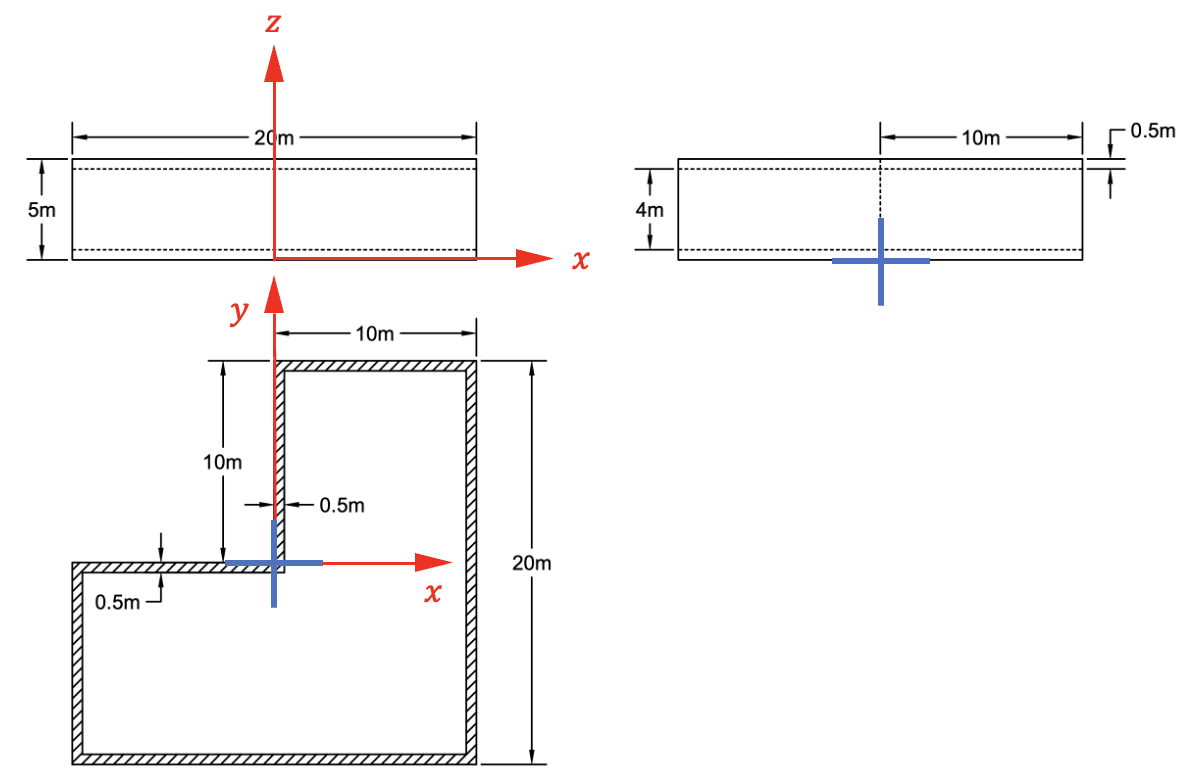
\includegraphics[scale=.45]{figures/empty_room_three_view.png}
	\caption{The three-viewed drawing of the empty room}
	\label{empty room three-view}
\end{figure}

\begin{figure}[t]
    \centering
    \begin{subfigure}{0.45\textwidth}
        \centering
        \adjustbox{height=5cm}{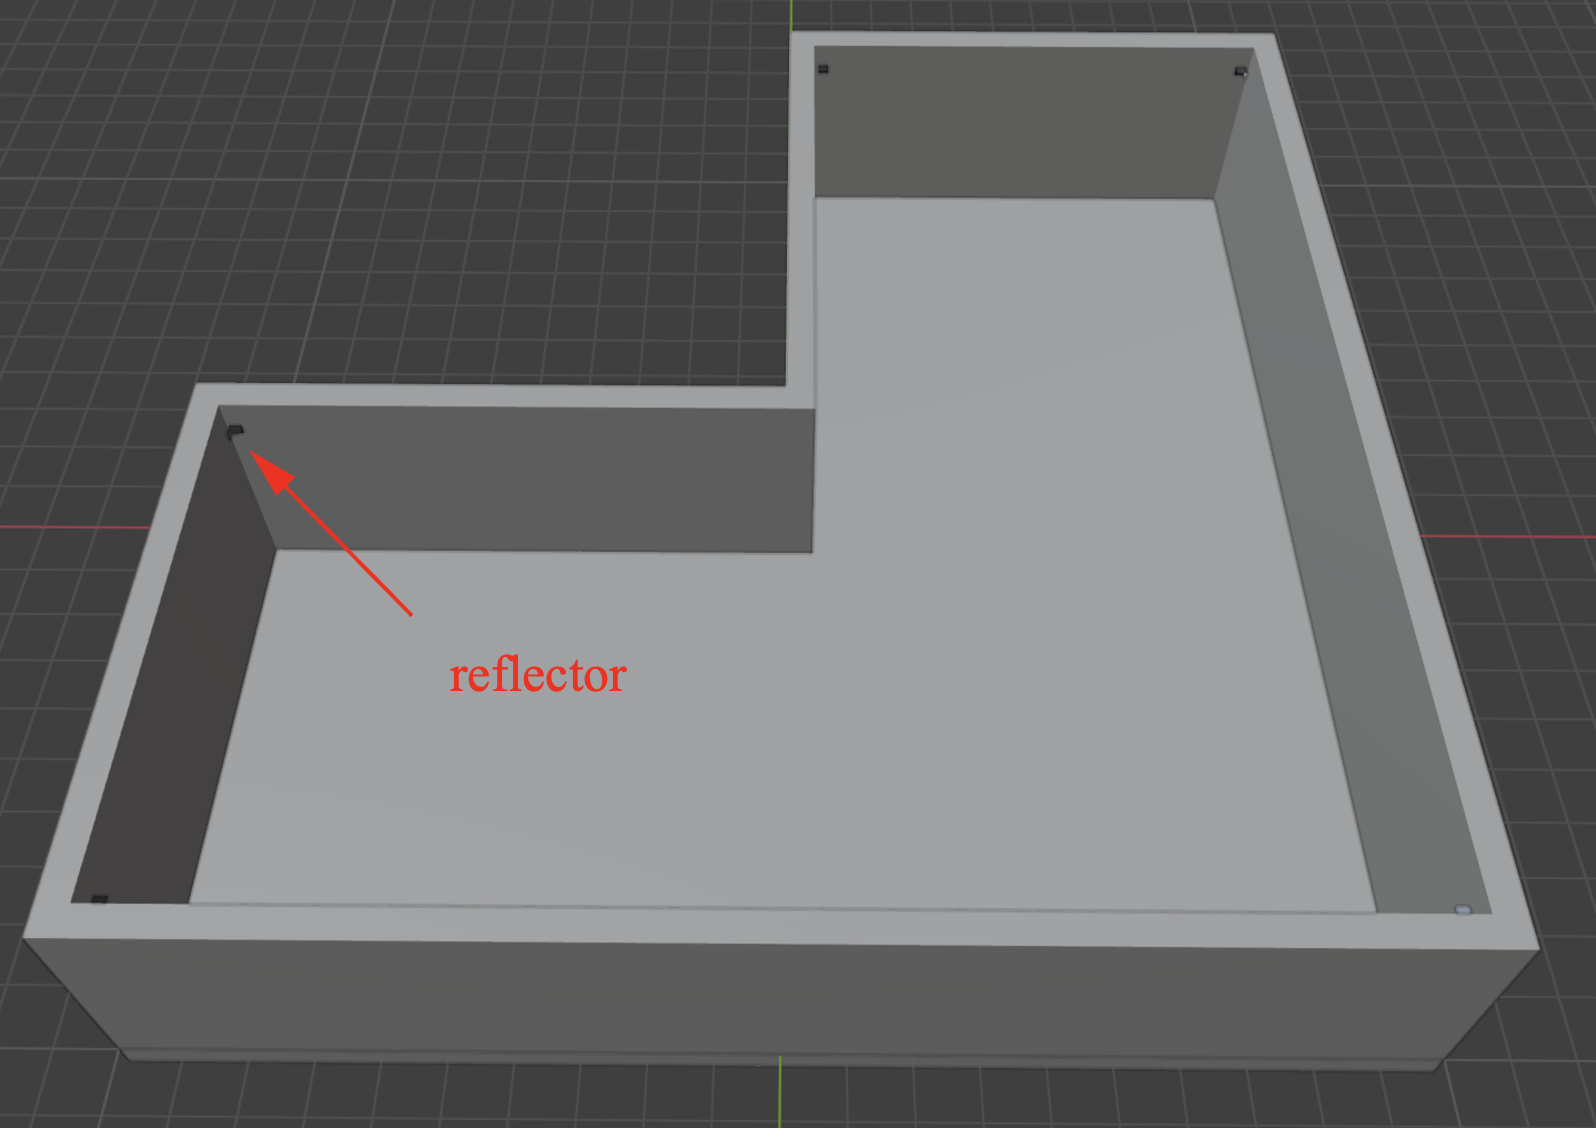
\includegraphics[width=\linewidth,scale=.3]{figures/empty_room_without_ceiling.png}}
    \end{subfigure}
    \begin{subfigure}{0.45\textwidth}
        \centering
        \adjustbox{height=5cm}{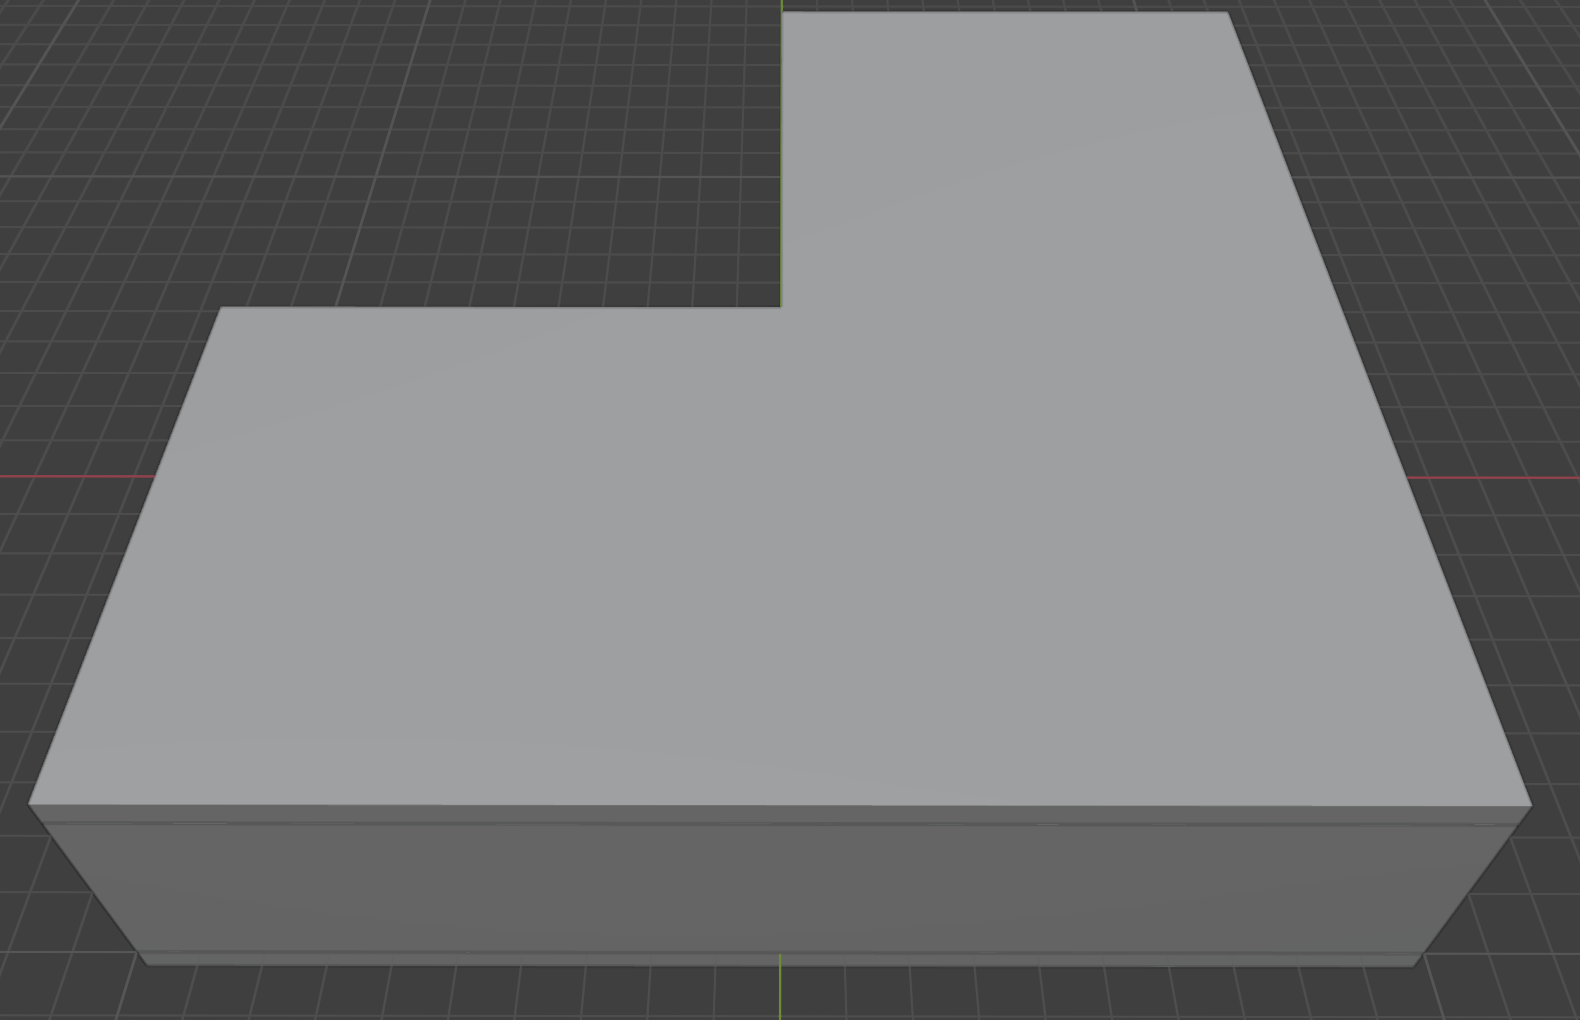
\includegraphics[width=\linewidth,scale=.3]{figures/empty_room_with_ceiling.png}}
    \end{subfigure}
    \caption{View of the empty room}
    \label{view of the empty room}
\end{figure}

\begin{spacing}{1.5}
\textbf{\large{Reflectors}}
\end{spacing}

For reflectors, two types of reflectors are used, one is the trihedral corner reflector and the other is the octahedral reflector. Due to angle limitations, trihedral corner reflectors can only be placed at the five corners of the room, while the octahedral reflector can be seen as multiple corner reflectors combined, so the range of incident angles is much wider. While testing the impact of the number of reflectors on the results later, different numbers and positions of octahedral reflectors can be set. The edge size of both triangular and octahedral reflectors is chosen as $20\,\mathrm{cm}$. To achieve its hanging, the reflector will be placed at least $0.5\,\mathrm{m}$ away from the wall.

Compared to the wall, the reflector's material selection is the opposite. All roughness values will be set to 0 and all metallic values will be set to 1 to achieve the full specular reflection. Additionally, the index of refraction (IOR) in the coat is set to 0 as well, because only the reflection is considered rather than refraction. But the IOR in the specular part is set as 1 to increase the reflection intensity.

At the corner of the left image in Figure \ref{view of the empty room} it shows where they are placed, and Figure \ref{view of the reflector} will show how the two reflectors will look in Blender.

\begin{figure}
    \centering
    \begin{subfigure}{0.45\textwidth}
        \centering
        \adjustbox{height=6cm}{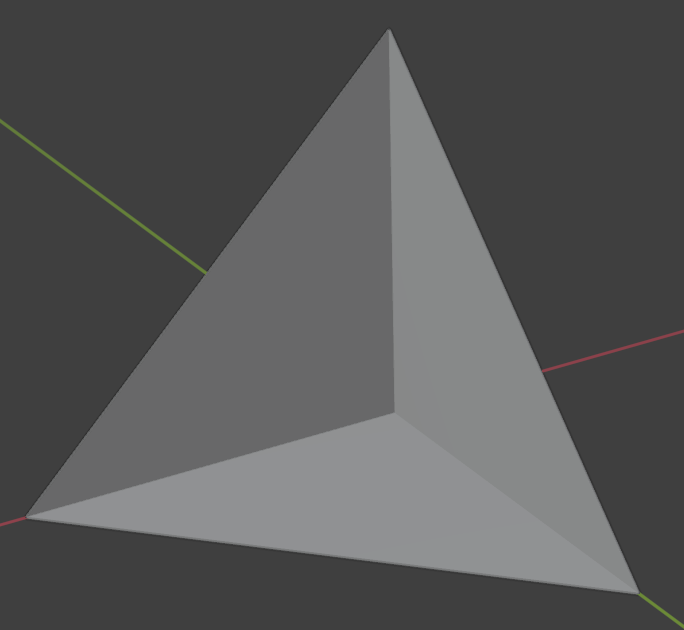
\includegraphics[scale=.3]{figures/tri_reflector.png}}
    \end{subfigure}
    \begin{subfigure}{0.45\textwidth}
        \centering
        \adjustbox{height=6cm}{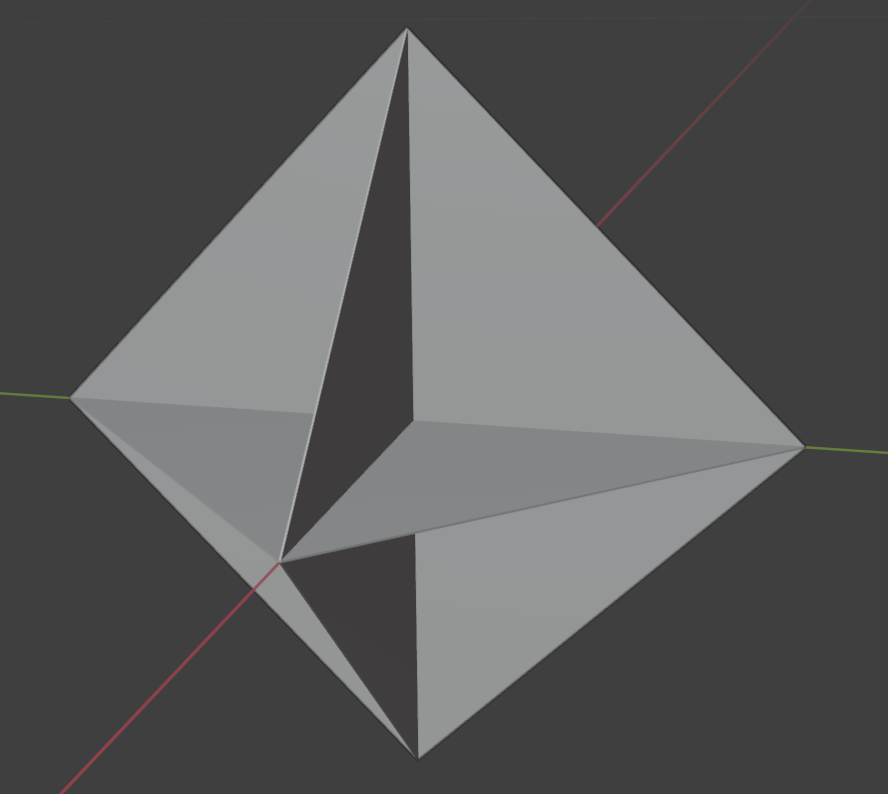
\includegraphics[scale=.3]{figures/octa_reflector.png}}
    \end{subfigure}
    \caption{View of the trihedral corner reflector on the left side and octahedral reflector on the right side}
    \label{view of the reflector}
\end{figure}

\begin{spacing}{1.5}
\textbf{\large{Room with furniture}}
\end{spacing}

In real scenario, the presence of furniture and other objects in the room affects the propagation of rays. For testing the impact of furniture and other objects on the target detection later, the room model with furniture is built. Many furniture models with material information are available for free online \cite{blender_furniture} and can be imported. However, due to the high hardware requirements of ray tracing and the increased complexity of object surfaces, this article only appropriately imports some furniture to research the relationship between them and the results. Figure \ref{view of the furniture} shows two room models with furniture, one on the right side with more furniture, and another one on the left side with less furniture. For the reason above, later the left model will be mainly simulated.

\begin{figure}
    \centering
    \begin{subfigure}{0.45\textwidth}
        \centering
        \adjustbox{height=6cm}{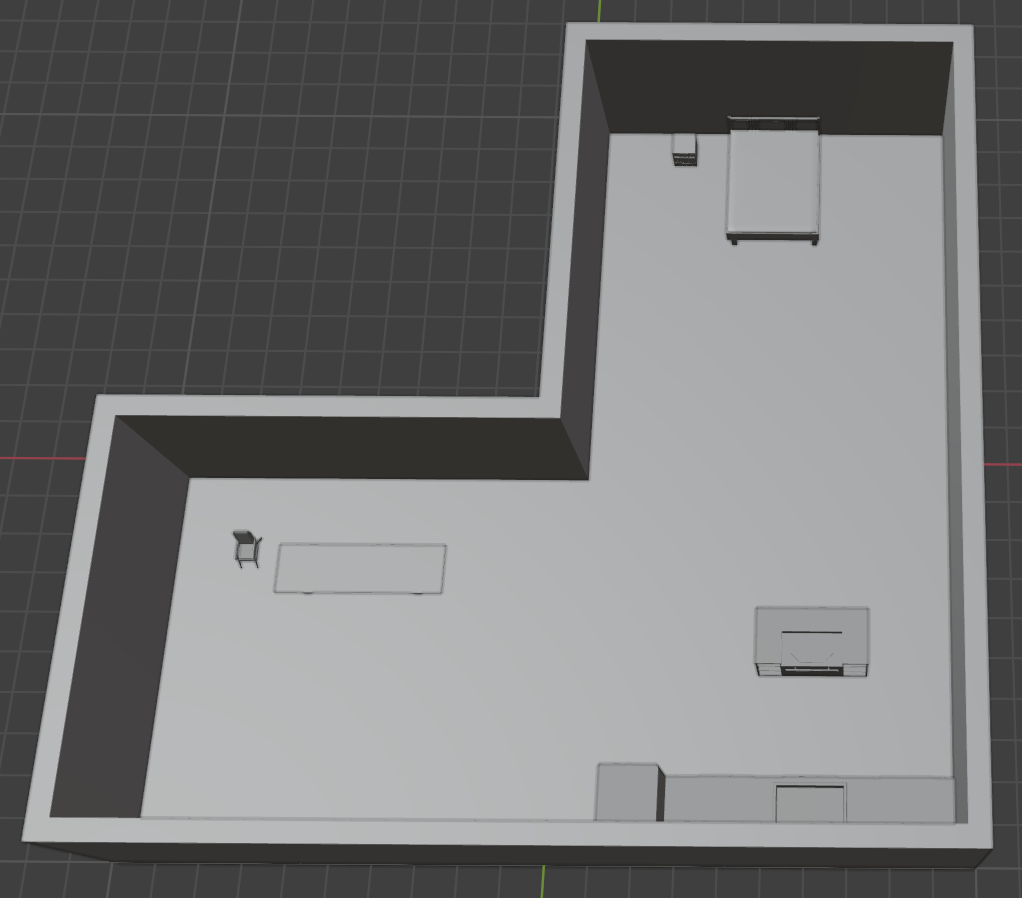
\includegraphics[scale=.3]{figures/furniture_simple.png}}
    \end{subfigure}
    \begin{subfigure}{0.45\textwidth}
        \centering
        \adjustbox{height=6cm}{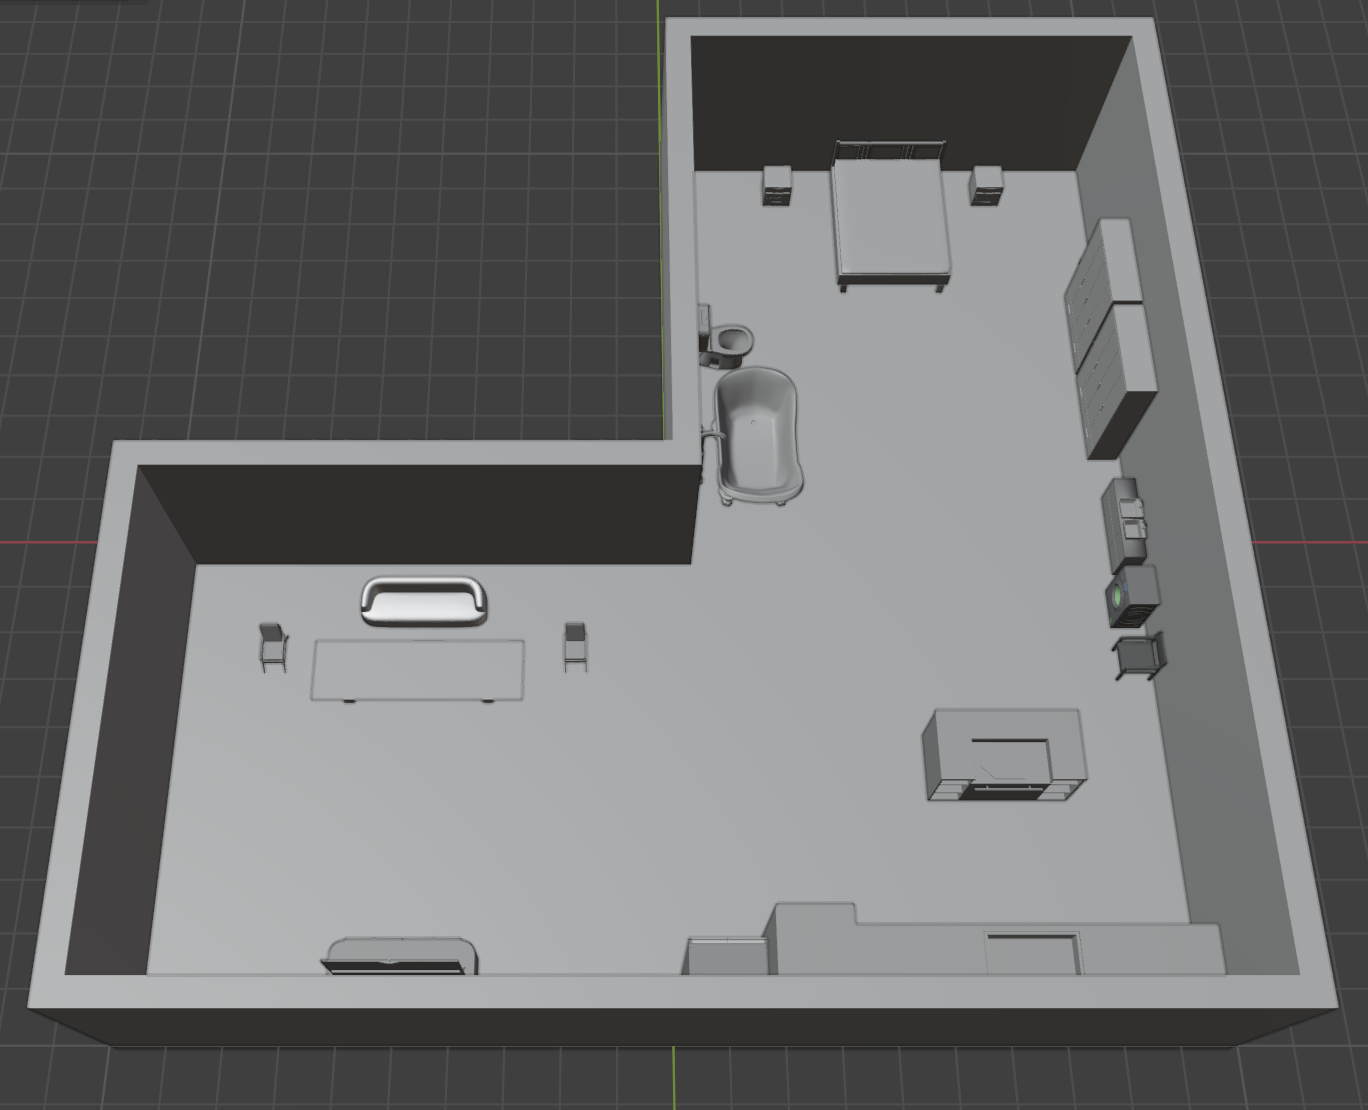
\includegraphics[scale=.3]{figures/furniture_complex.png}}
    \end{subfigure}
    \caption{View of the room model with furniture}
    \label{view of the furniture}
\end{figure}

\begin{spacing}{1.5}
\textbf{\large{Plausibility check}}
\end{spacing}

During the modeling of the room, raytracing as well as the signal processing, in order to verify whether the raytracing effect meets expectations and to determine if the obtained range and velocity are reasonable, a standalone wall with a reflector mounted in one corner is built. Then the process of the plausibility check goes as following: the antenna can be placed in front of the wall, with the given position and velocity. By observing the propagation path of rays and the resulting signal processing, the interval between the results and the given values could be checked in terms of range, as well as the magnitude and direction of velocity. This allows us to verify the correctness of the results throughout this process.

Figure \ref{view of the plausibility check} shows two types of plausibility models, one on the left side is one wall that could be used for testing the reflection of the wall and the range, while another one on the right with an additional reflector is mainly used for testing the velocity relative to the reflector. 

\begin{figure}
    \centering
    \begin{subfigure}{0.45\textwidth}
        \centering
        \adjustbox{height=6cm}{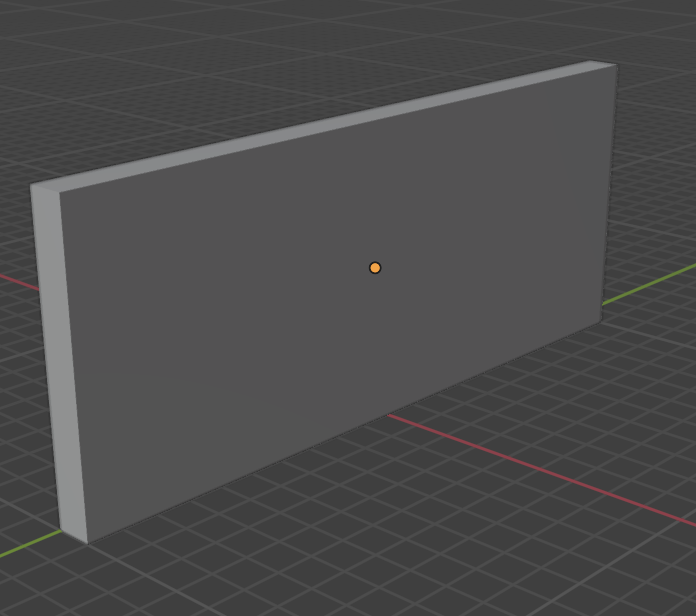
\includegraphics[scale=.3]{figures/wall.png}}
    \end{subfigure}
    \begin{subfigure}{0.45\textwidth}
        \centering
        \adjustbox{height=6cm}{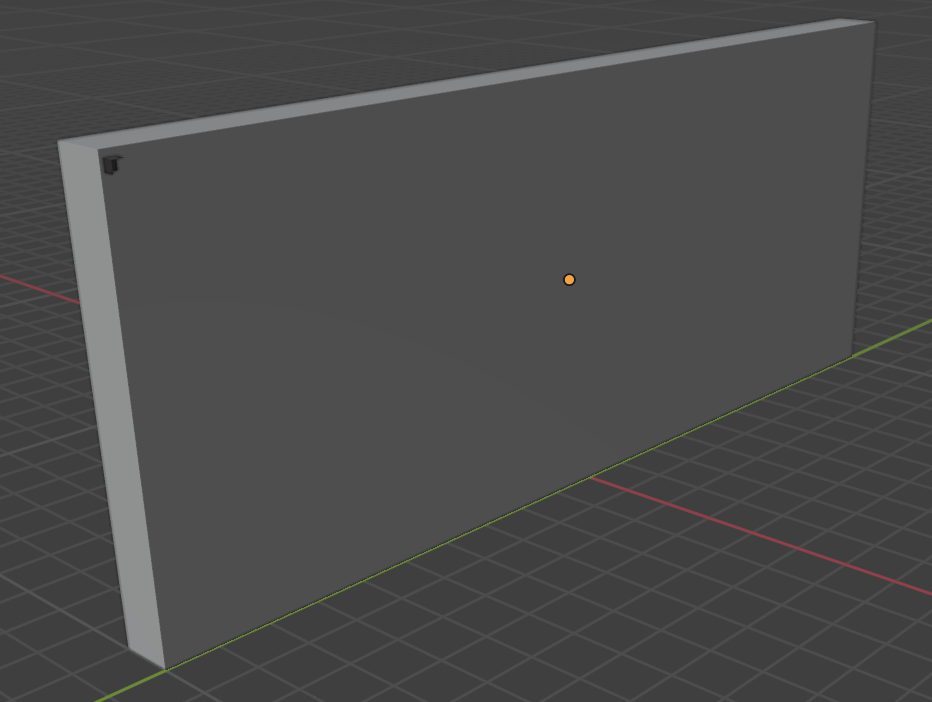
\includegraphics[scale=.3]{figures/wall_with_reflector.png}}
    \end{subfigure}
    \caption{View of the plausibility check model}
    \label{view of the plausibility check}
\end{figure}

\subsection{Matlab raytracer} \label{Matlab raytracer}

\begin{spacing}{1.5}
\textbf{\large{Setup}}
\end{spacing}

For the parameters in ray tracing, in addition to the parameters calculated and chosen in Table \ref{parameters of the radar system}, there are some other setting values \cite{raytracer_input}:

\begin{enumerate}[label=\textbullet]
    \item The position of the robot is set as $(3, -2, 0.5)\,\mathrm{m}$ by default, as the antennas are assumed to be packaged on the same platform, so they are quite near. So in this case, the position of the transmitter is chosen the same as the robot, and then quasi-monostatic receive is placed with a location difference of $1\,\mathrm{mm}$ in x- and y direction from the transmitter antenna.

    \item For the robot's velocity, if it is stationary, use $v = [0, 0, 0]$. Otherwise, to detect the effect of its velocity on the range-Doppler map later, use $v = [1, 2, 0]$ by default.

    \item For the orientation of the antenna, the radiation pattern of the antenna is assumed to be isotropic currently, but the anisotropic radiation pattern will be added later, as the orientation of the robot has a great influence on the gain value. Since we use quaternion for the orientation of the robot and if there is no rotation, the orientation is set as $[1, 0, 0, 0]$ by default. Later in section \ref{Antenna radiation pattern}, we will get its orientation in real-time according to the robot's motion trajectory.

    \item In the simulation process, we only set the scene in the built room model, and the coordinates are set according to the red cross in Figure \ref{empty room three-view} as the origin. Therefore, to do the ray tracing, the coordinate system is chosen as "cartesian" for both the transmitter and receiver site.

    \item The important simulation limitation in ray tracing includes setting the maximum number of reflections (MaxNumreflections), the maximum number of diffractions (MaxNumDiffractions), the maximum relative path loss (MaxRelativePathLoss), the maximum absolute path loss (MaxAbsolutePathLoss), and so on. The maximum relative path loss refers to the loss threshold of all rays relative to the strongest ray. Due to the uncertainty of the trajectory, the robot may be too close to an object, resulting in the strongly reflected rays and the relatively weaker rays back from the reflectors. Therefore, it is difficult to determine a relative threshold, so this part does not set a threshold, i.e. set as "Inf". For the rays which has a large path loss, even if the ray is simulated in ray tracing, it has still relatively little significance in subsequent signal processing and range Doppler map. This is why we mainly focused on the $10\,\mathrm{m}$ range in our earliest parameter selection, so here we set these three values as $MaxNumreflections = 4$, $MaxNumDiffractions = 1$, and $MaxAbsolutePathLoss = 150\,\mathrm{dB}$ due to the computational complexity and simulation duration.

    \item In the ray tracing method, there are two options, namely shooting and bouncing ray (SBR) and image. In our system, the SBR method \cite{ray_tracer_inputs} is chosen which combines geometric optics and physical optics. Compared with the image method, it can better estimate the trajectory path of rays in the scene considering different types of interactions accurately. Meanwhile, the processing speed is faster, which is conducive to the simulation of complex scenes. Additionally, it is very important that the SBR method can support up to 10 reflections, while the image method only supports up to two. In our setting, we want to achieve up to 4 reflections, so the SBR method would be a better choice.

    The principle of SBR is that the position of the transmitter is assumed as the center of a sphere and it transmits rays outward uniformly, traces the path of each ray, and observes the interaction between it and the surrounding objects, including reflection, refraction, diffraction, and scattering. However, the problem is that Matlab can only trace edge diffraction but without surface diffraction of objects. When the ray hits a smooth surface, which means mainly reflectors or sometimes the walls in our system, it will be reflected according to the law of reflection. While hitting the edge of an object, a new diffraction ray will be generated according to the law of diffraction, and the new diffraction point will be the new transmitting center. For receiving rays, a sphere is formed with the position of the receiver as the center. If the ray intersects the sphere, it is considered that the path of this ray is valid from the transmitter to the receiver. Figure \ref{the sbr method in raytracer} illustrates the principle of the SBR method in raytracer.

    \begin{figure}
    	\centering
    	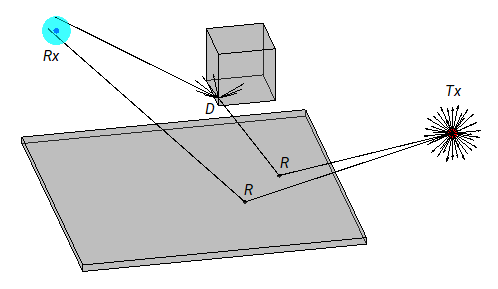
\includegraphics[scale=.5]{figures/ray_tracing_sbr_method.png}
    	\caption{The SBR method in raytracer \cite{ray_tracer_inputs}}
    	\label{the sbr method in raytracer}
    \end{figure}

    \item Another parameter is the separation of angle. As the angle between rays emitted by the transmitter decreases, the number of emitted rays will increase, and the simulation effect will be more realistic. However, the reduction of the angle also increases the hardware requirements and the running time. Therefore, as a compromise, the angle is set as 0.5 degrees.

    \item Material properties can also be set in Matlab's ray tracing if the imported object does not have material information. Since the room and reflector imported from Blender have material information already, but other imported furniture may have missing information, a relatively rough surface, i.e. concrete, is selected for the unset parts.
\end{enumerate}

\begin{spacing}{1.5}
\textbf{\large{Raytracer}}
\end{spacing}

This part will implement the above settings in Matlab and show the view of its simulation as well as its impact through the comparison of different scenes, including the effect of reflectors, the effect of furniture, and the plausibility check.

\begin{enumerate}[label=\textbullet]
    \item View of the ray tracing in the empty room
    
    Figure \ref{view of the ray tracing in the empty room} shows the effect of the ray tracing in the empty room. The color of the rays represents the magnitude of the path loss, and as the loss increases, the color changes from dark red to dark blue. In the empty room, if there is no reflector, no furniture, and all pattern is isotropic, the color is basically blue and the loss is usually around $130\,\mathrm{dB}$. There are some observations that the shorter the propagation distance or the fewer number of the reflections and diffractions, the lighter the color, which means the less loss, and the rays are located on the vertical plane between the transmitter and the walls.

    \begin{figure}
    \centering
    \begin{subfigure}{0.45\textwidth}
        \centering
        \adjustbox{height=5.2cm}{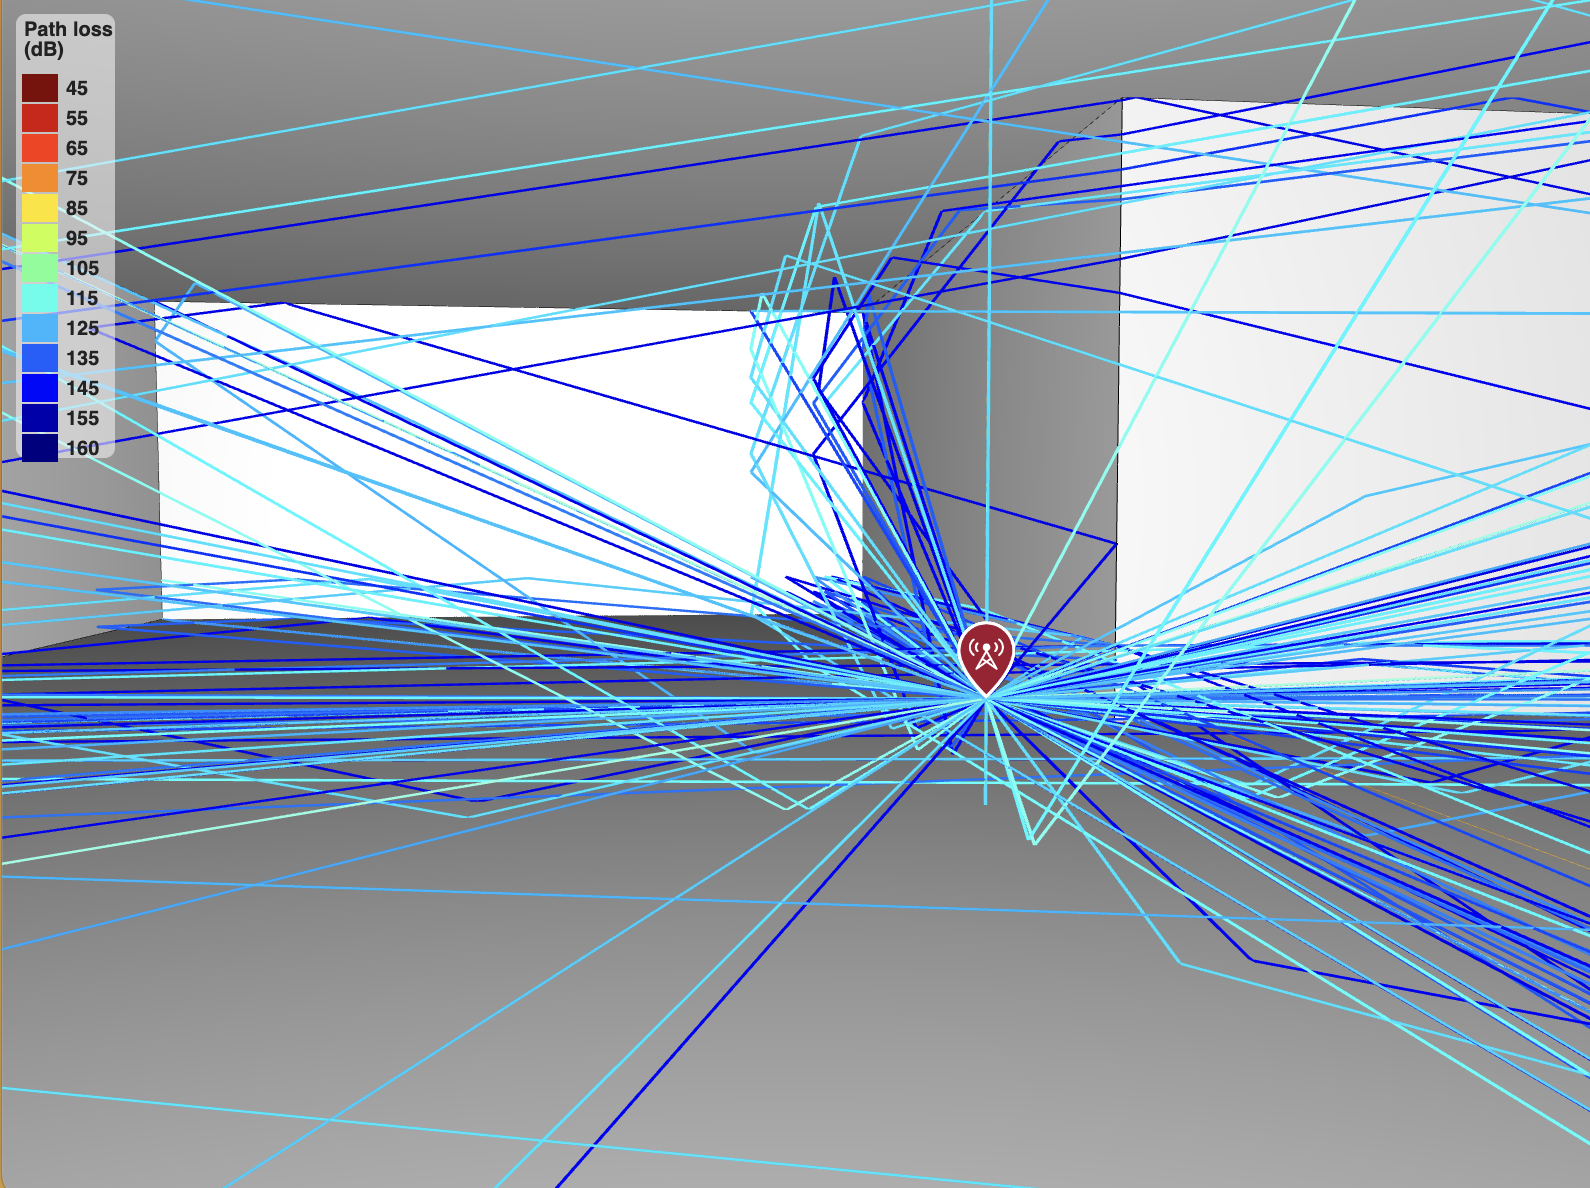
\includegraphics[scale=.3]{figures/empty_room_simulation_left.png}}
    \end{subfigure}
    \begin{subfigure}{0.45\textwidth}
        \centering
        \adjustbox{height=5.2cm}{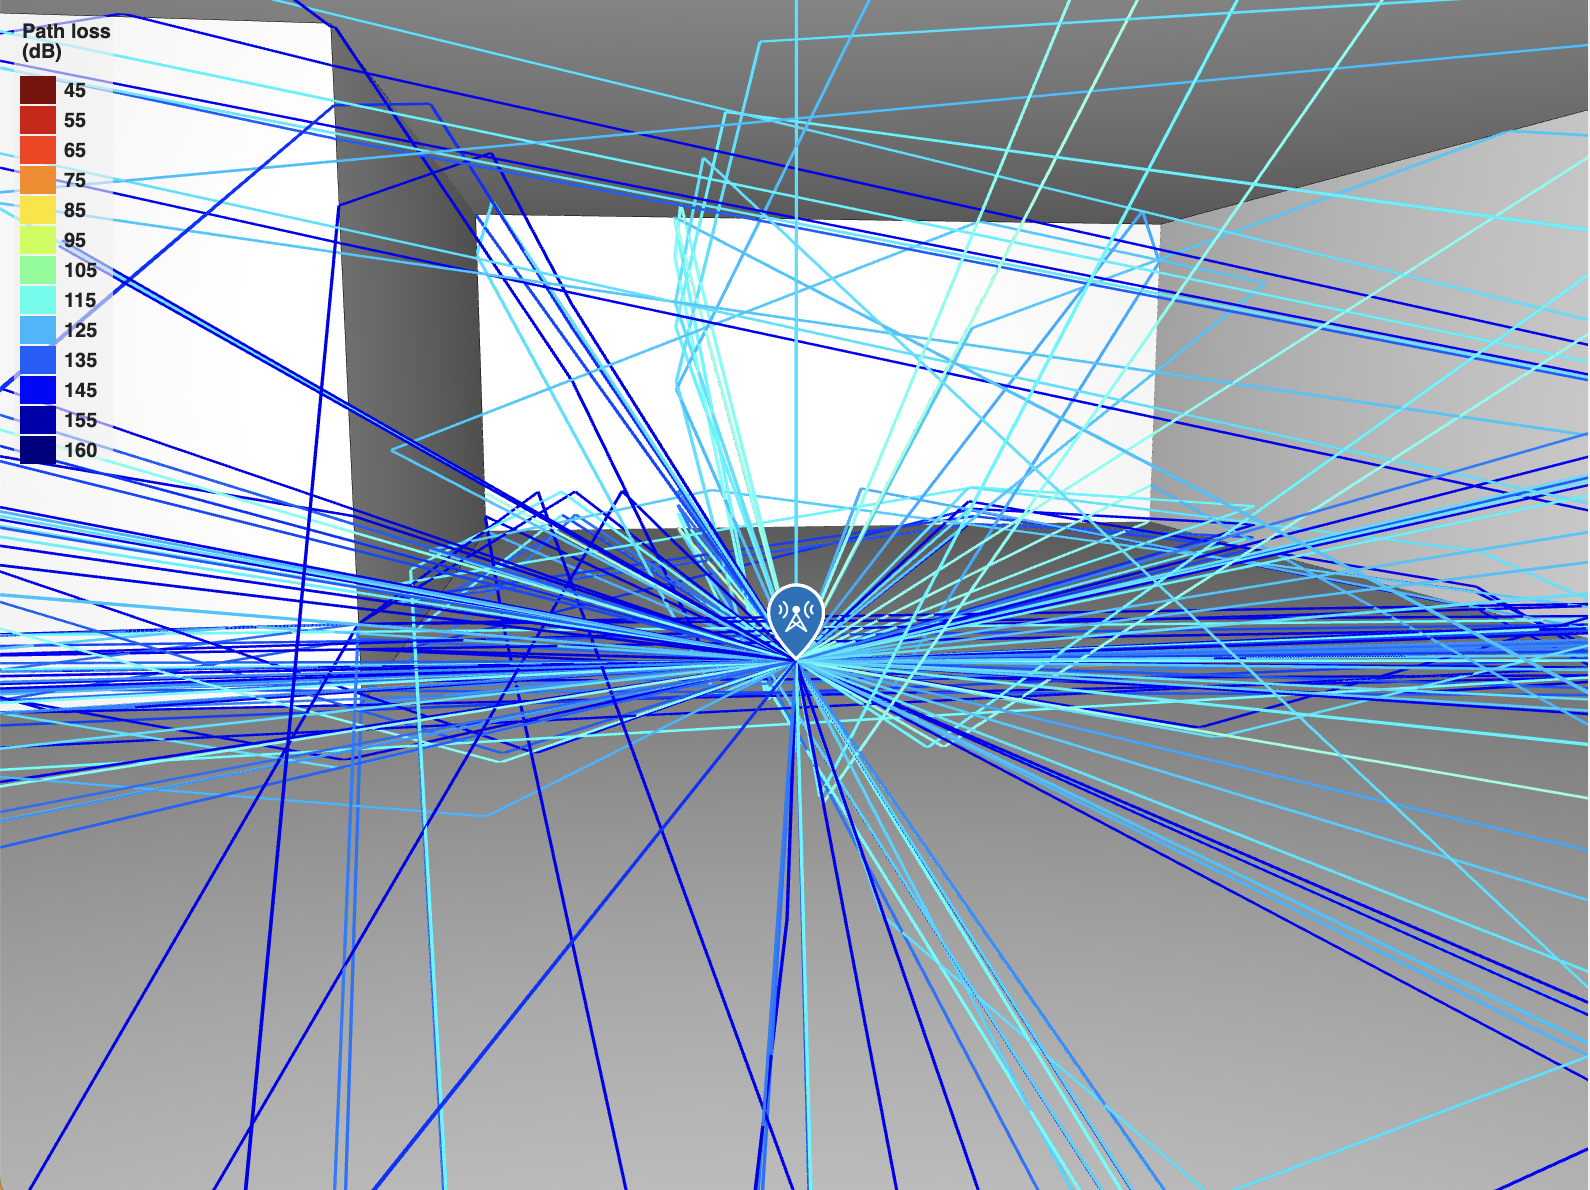
\includegraphics[scale=.3]{figures/empty_room_simulation_right.png}}
    \end{subfigure}
    \caption{View of the ray tracing in the empty room}
    \label{view of the ray tracing in the empty room}
    \end{figure}

    \item The effect of the reflectors in the ray tracing

    Figure \ref{the effect of the reflectors in ray tracing} shows the effect of the reflectors after hanging at the corner of the empty room. Compared with the case above, the color of the rays is still mostly blue, but the path of the rays is currently not just on the plane orthogonal to the walls. As seen in Figure \ref{the effect of the reflectors in ray tracing}, there are currently beams of rays between the transmitter and reflectors, where the loss with this propagation distance in the above case will be over the $140\,\mathrm{dB}$ threshold.

    But there is a compromise with current reflectors. As the reflector's edge length grows, the value of the radar cross-section will be higher, making it more obvious in subsequent range-Doppler maps. But the problem is that, as shown in Figure \ref{reflections_inside_reflector}, the increase in size leads to multiple reflections inside the reflector, causes more rays propagating through the reflectors, then the path losses of these rays are still too high to have influence on the result. Ideally, there should be a huge amount of rays all over the reflector but due to the lack of the surface diffraction, especially the strong rays from reflectors are out of simulation.

    \begin{figure}[t]
    \centering
    \begin{subfigure}{0.45\textwidth}
        \centering
        \adjustbox{height=5.2cm}{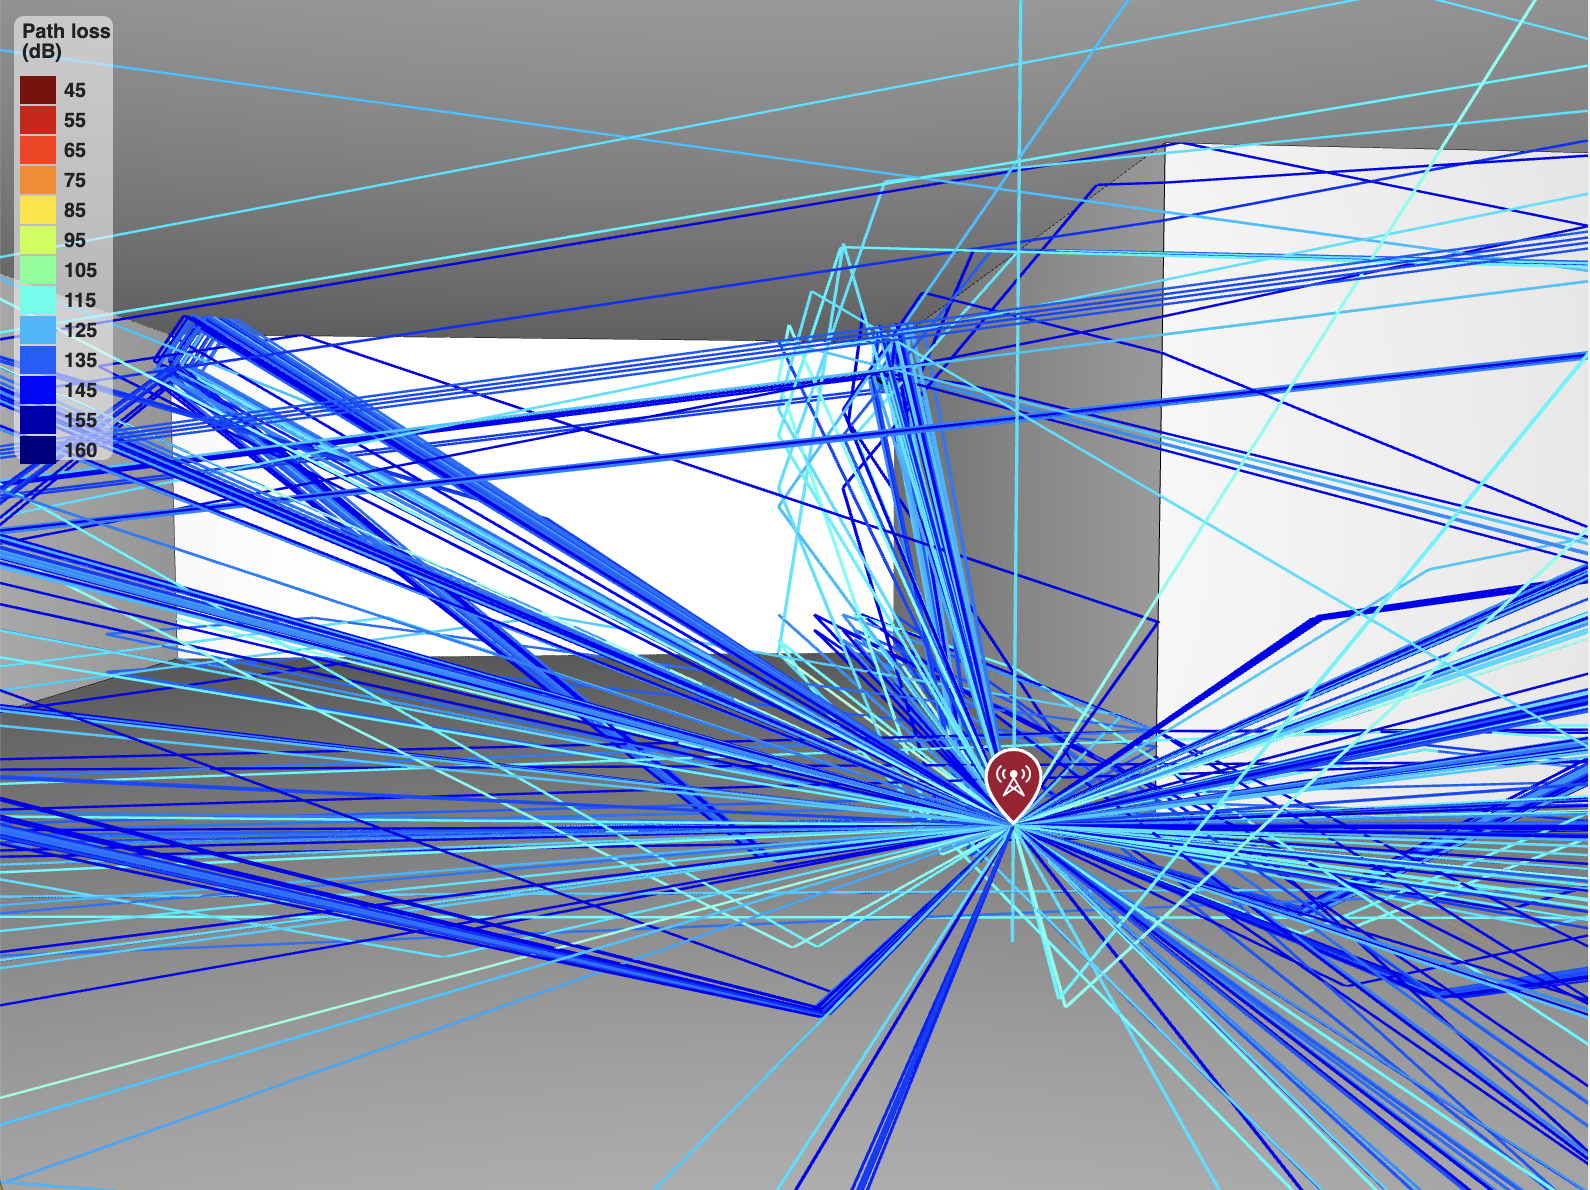
\includegraphics[scale=.3]{figures/reflector_simulation_left.png}}
    \end{subfigure}
    \begin{subfigure}{0.45\textwidth}
        \centering
        \adjustbox{height=5.2cm}{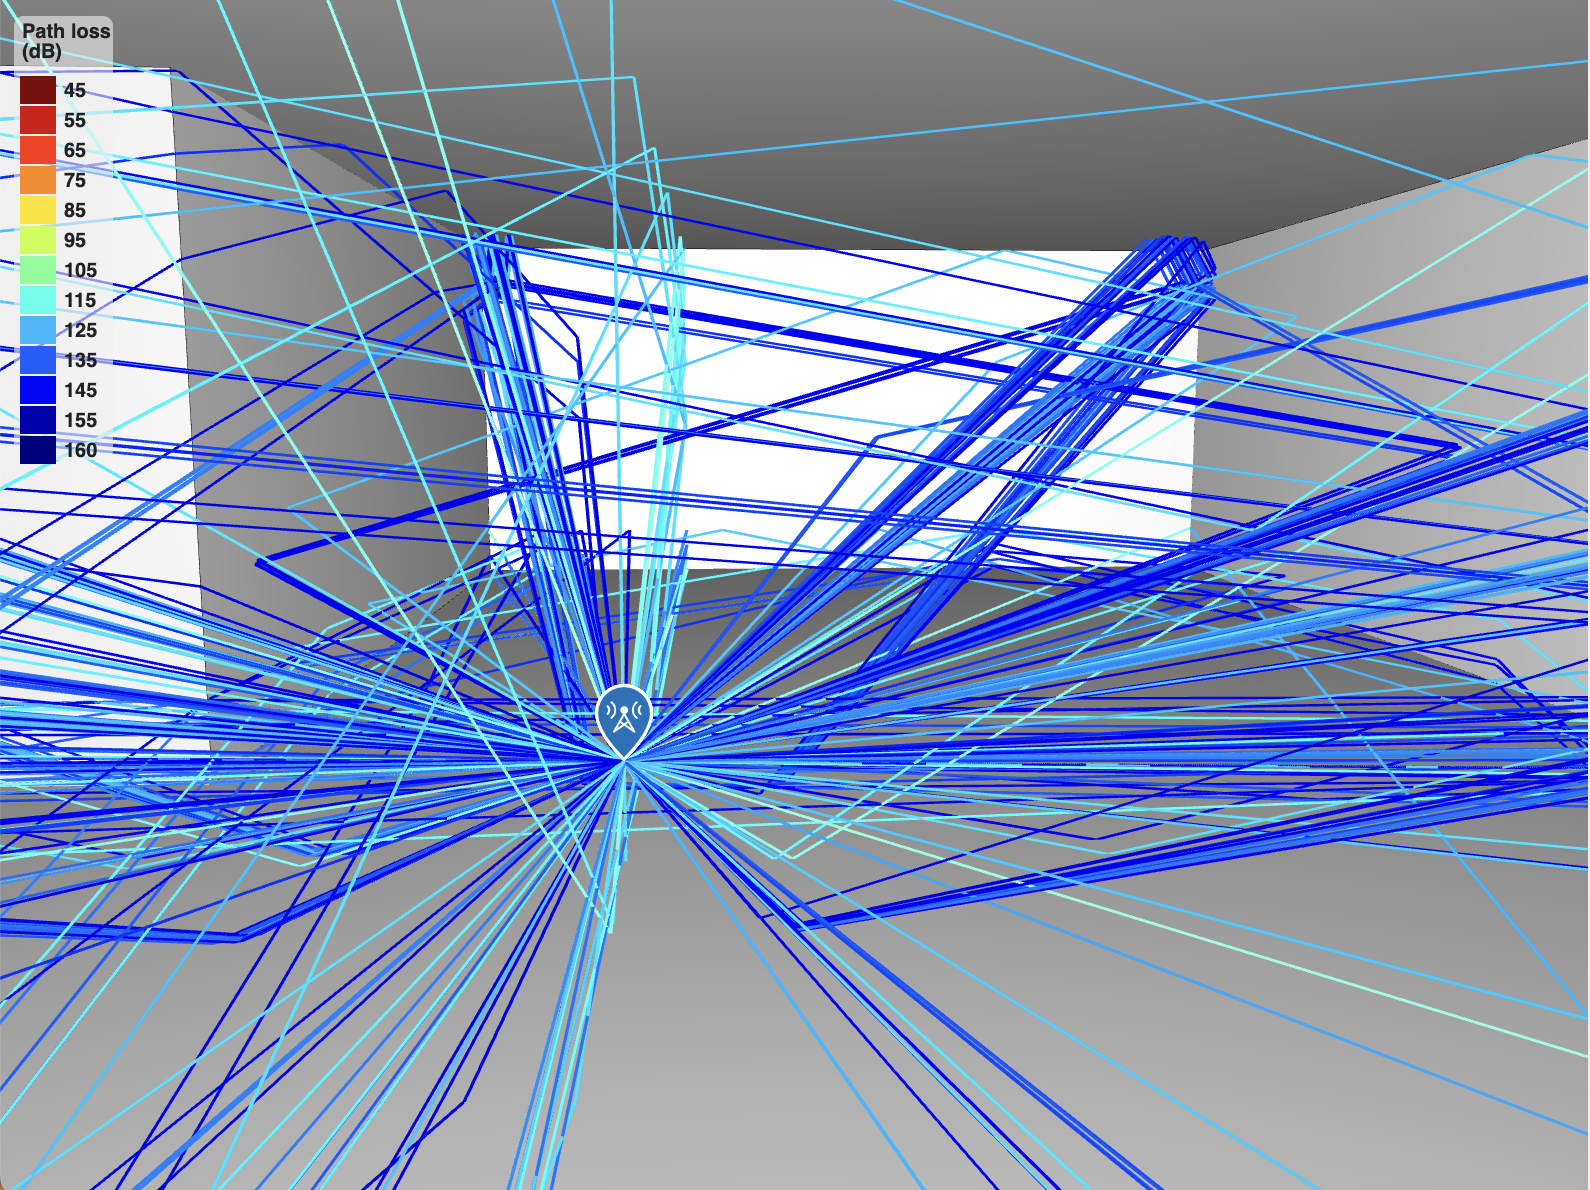
\includegraphics[scale=.3]{figures/reflector_simulation_right.png}}
    \end{subfigure}
    \caption{The effect of the reflectors in ray tracing}
    \label{the effect of the reflectors in ray tracing}
    \end{figure}

    \begin{figure}
	\centering
	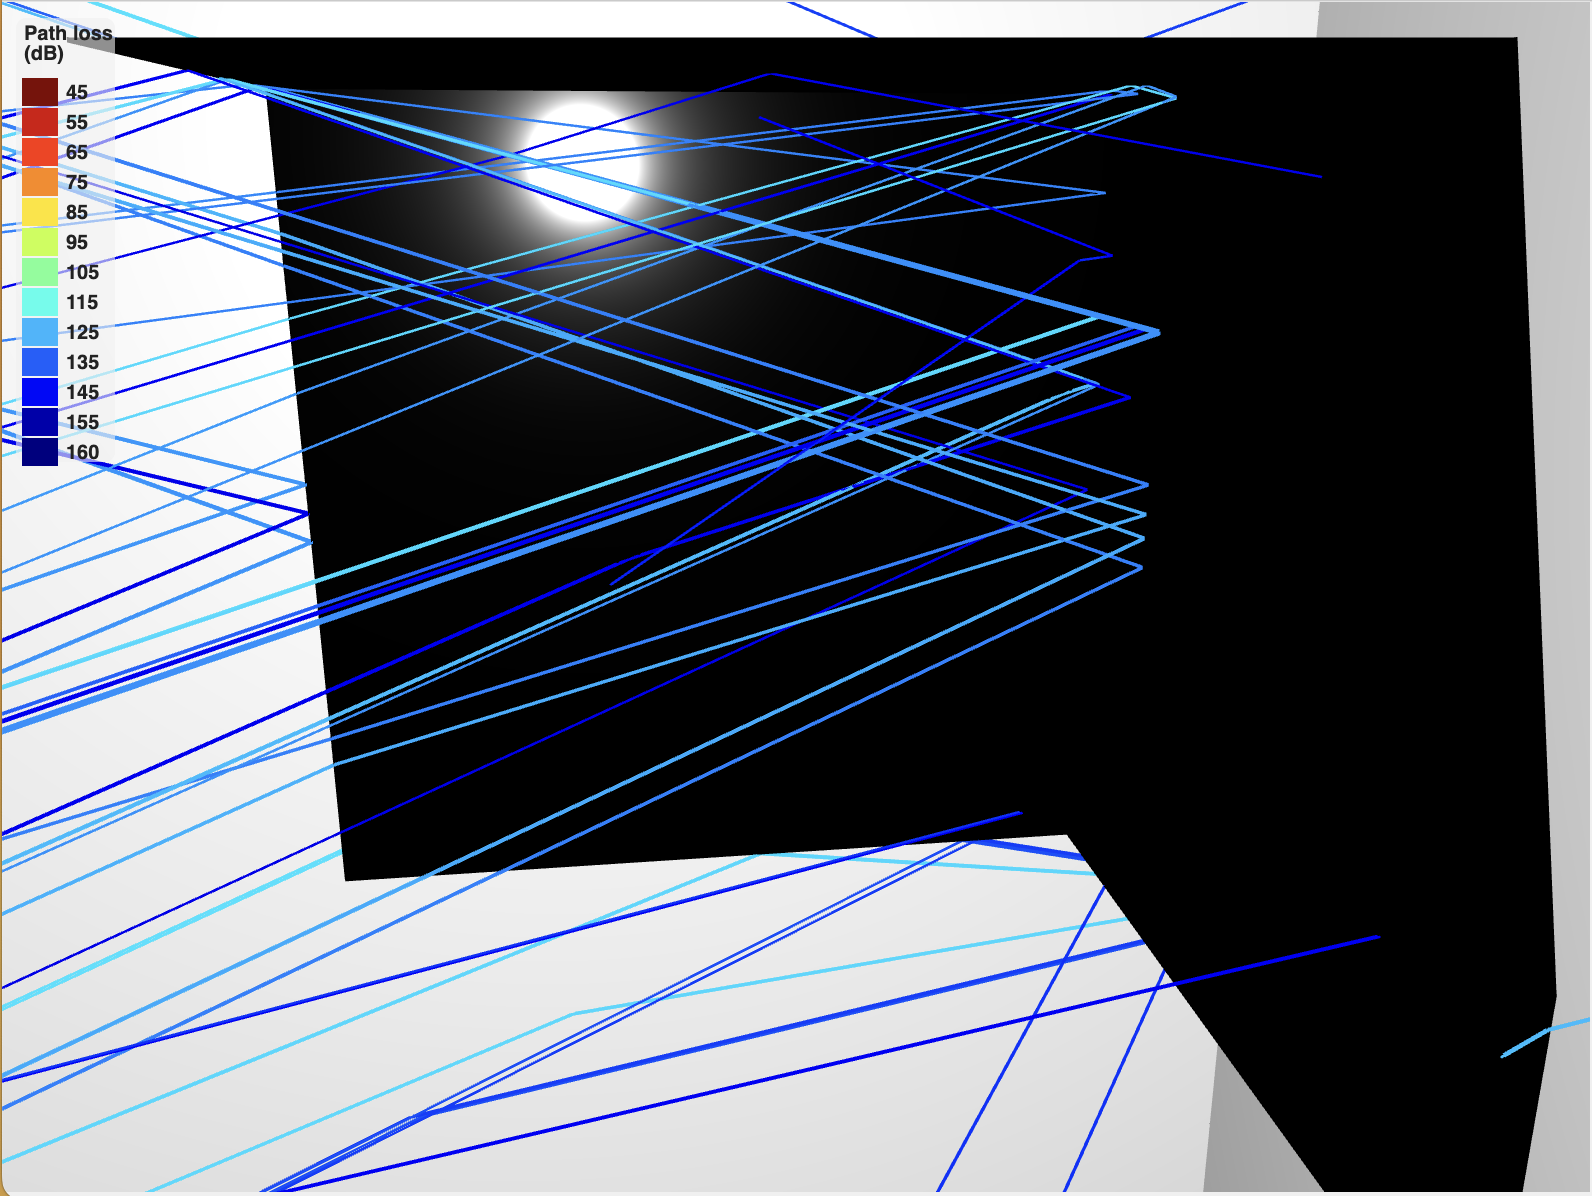
\includegraphics[scale=.3]{figures/reflections_inside_reflector.png}
	\caption{The reflections inside a reflector}
	\label{reflections_inside_reflector}
    \end{figure}

    \item The effect of the furniture in the ray tracing

    Figure \ref{the effect of the furniture in ray tracing} shows the effect of the furniture in the ray tracing. As seen in the figure, with the addition of the furniture, the path of the rays has more possibilities. However, during the motion of the robot, it is very likely to be too close to an object, resulting in more target points and stronger rays reflected by objects, which has effect on the subsequent signal processing process and the range Doppler map.

    \begin{figure}[t]
    \centering
    \begin{subfigure}{0.45\textwidth}
        \centering
        \adjustbox{height=5.2cm}{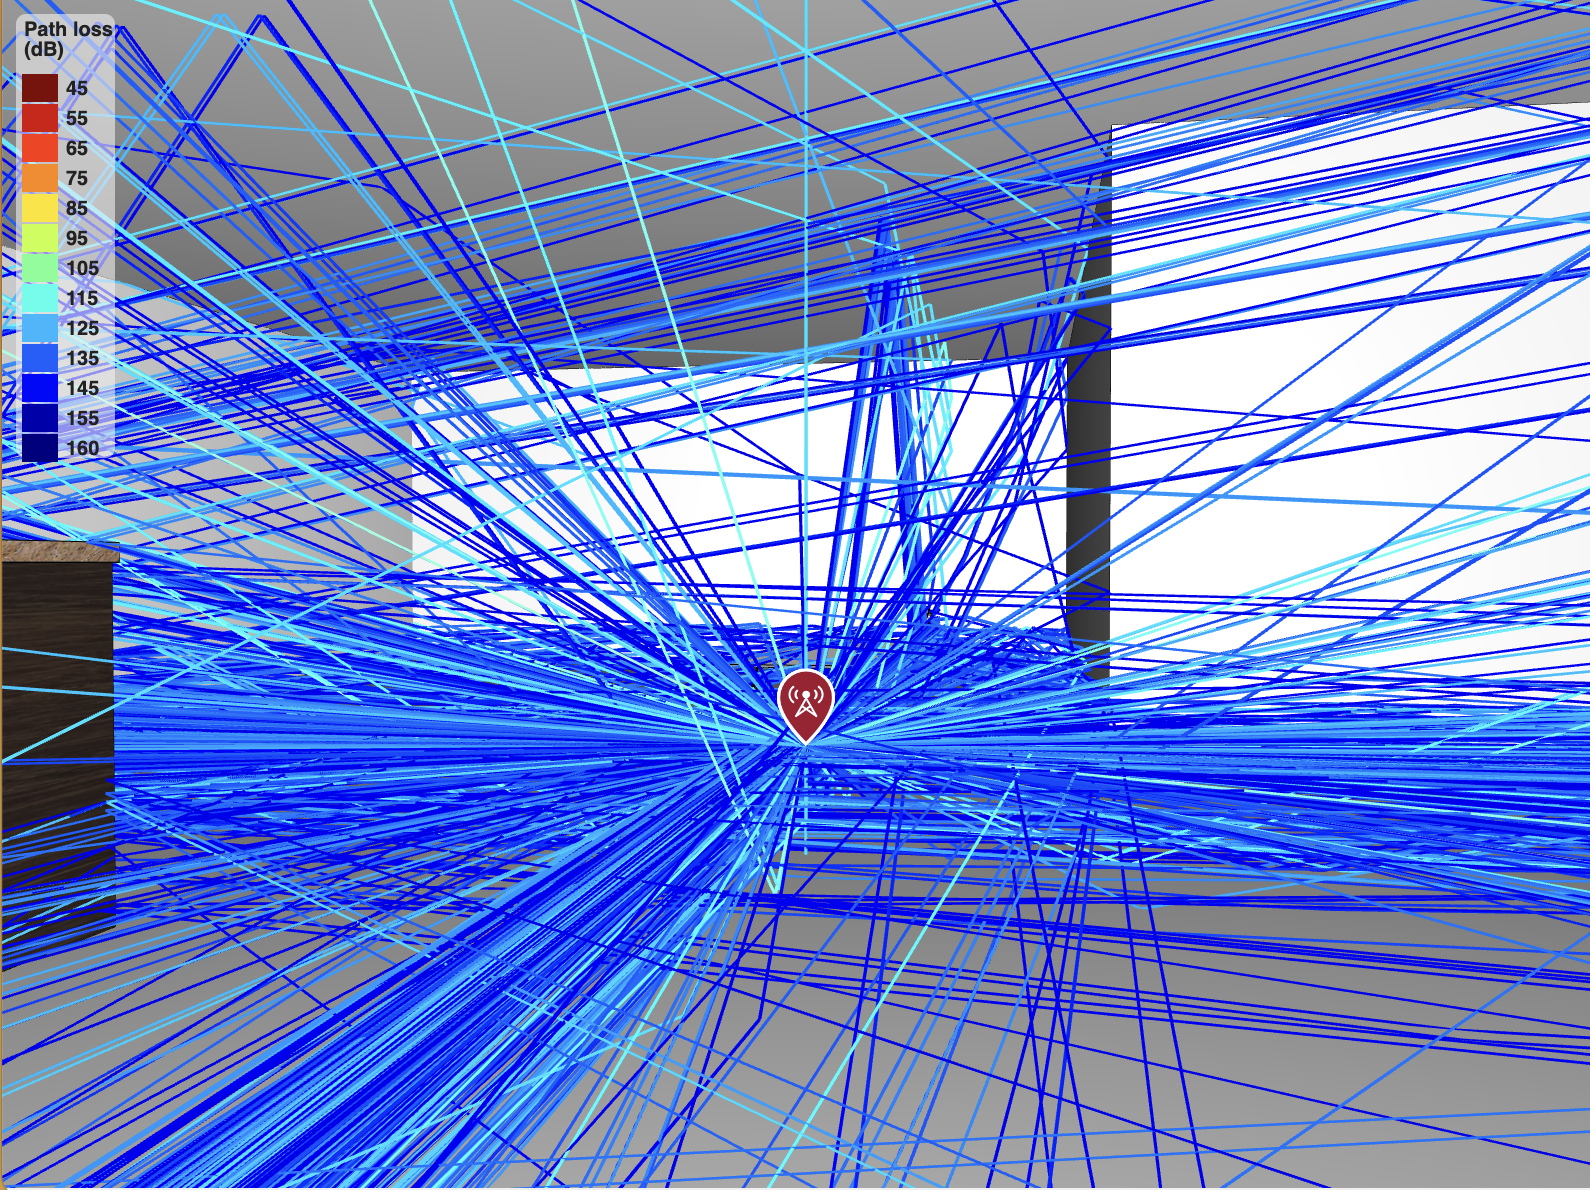
\includegraphics[scale=.3]{figures/furniture_simulation_left.png}}
    \end{subfigure}
    \begin{subfigure}{0.45\textwidth}
        \centering
        \adjustbox{height=5.2cm}{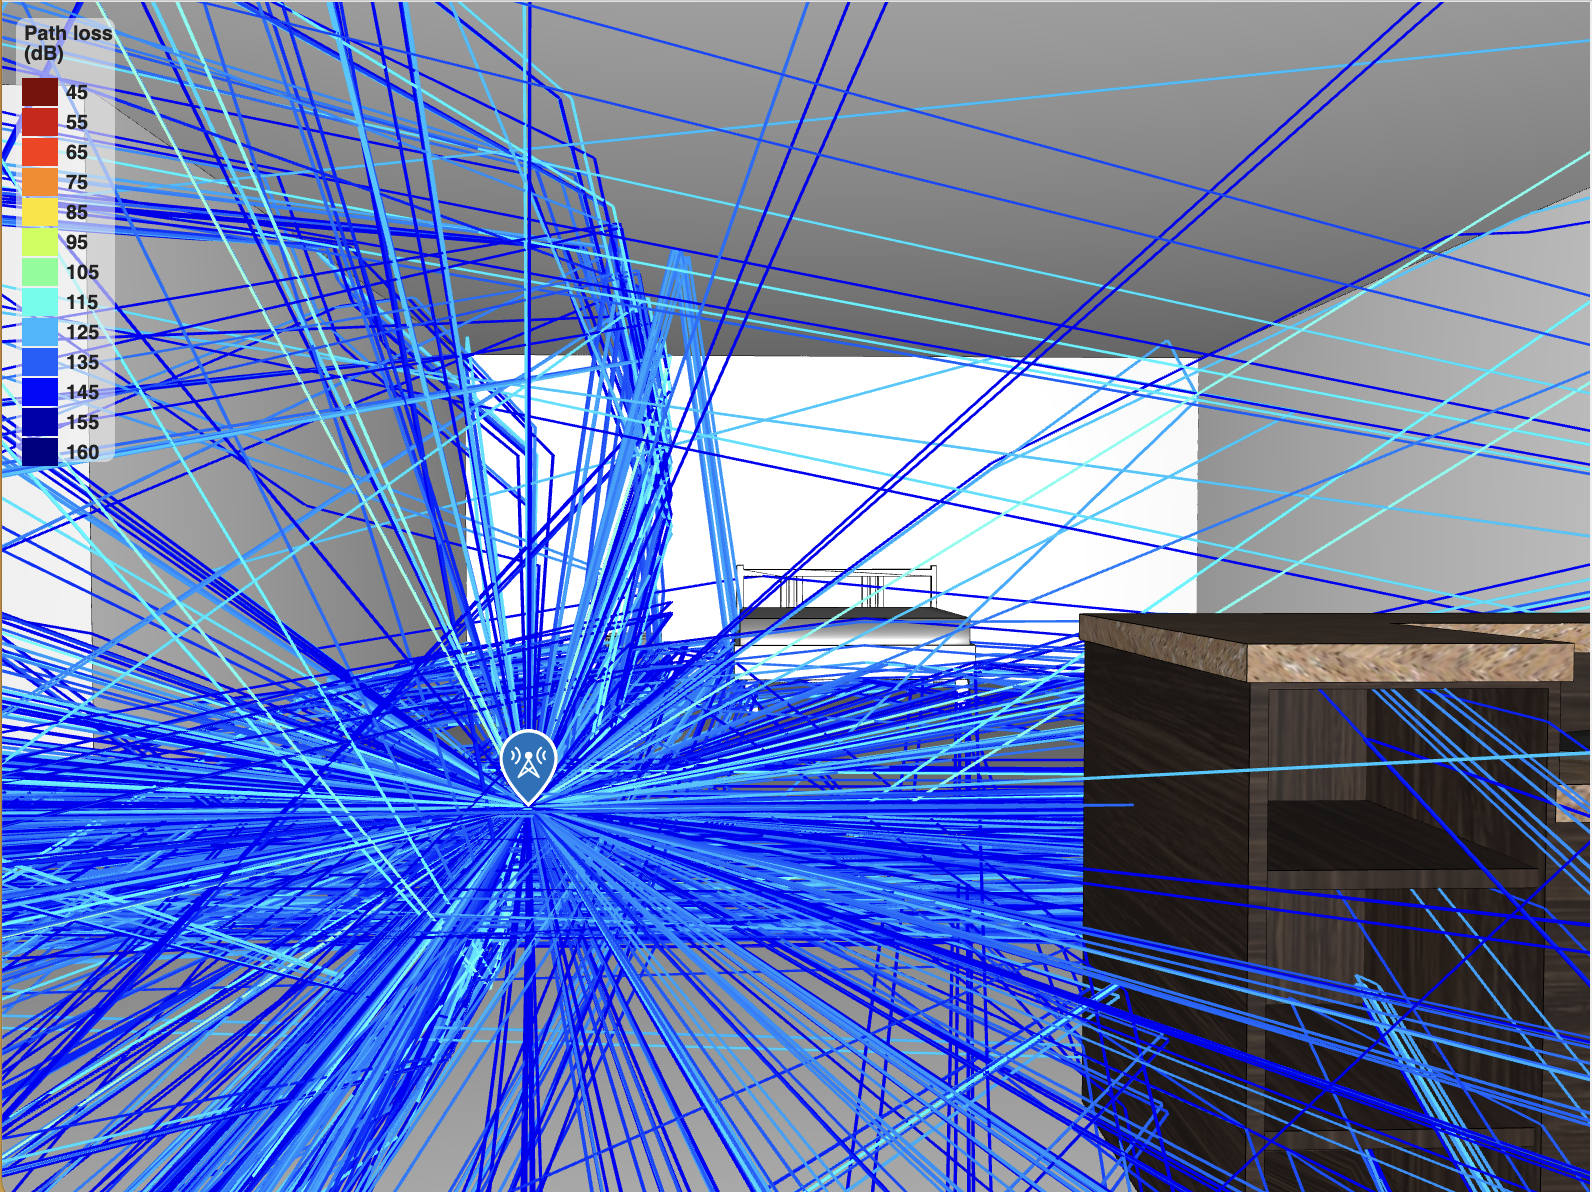
\includegraphics[scale=.3]{figures/furniture_simulation_right.png}}
    \end{subfigure}
    \caption{The effect of the furniture in ray tracing}
    \label{the effect of the furniture in ray tracing}
    \end{figure}

    \item View of the plausibility check in ray tracing

    Figure \ref{view of the plausibility check in ray tracing} shows the view of the plausibility check in ray tracing. On the left side, there is only one wall in front of the robot, which can be used for testing the propagation range. The interval is determined as $3\,\mathrm{m}$, and then we check the propagation distance of that yellow ray and determine whether the ray tracing system is correct or not. On the right side of the figure, there's one more reflector, which is used for checking the velocity relative to the reflector. If the position and velocity of the robot are given, then the relative velocity and distance could be calculated by hand, and compared with the properties of the rays and range Doppler map. As a close look seen in the right figure, the rays are generated due to multiple reflections rather than directly surface diffraction.

    \begin{figure}
    \centering
    \begin{subfigure}{0.45\textwidth}
        \centering
        \adjustbox{height=5.2cm}{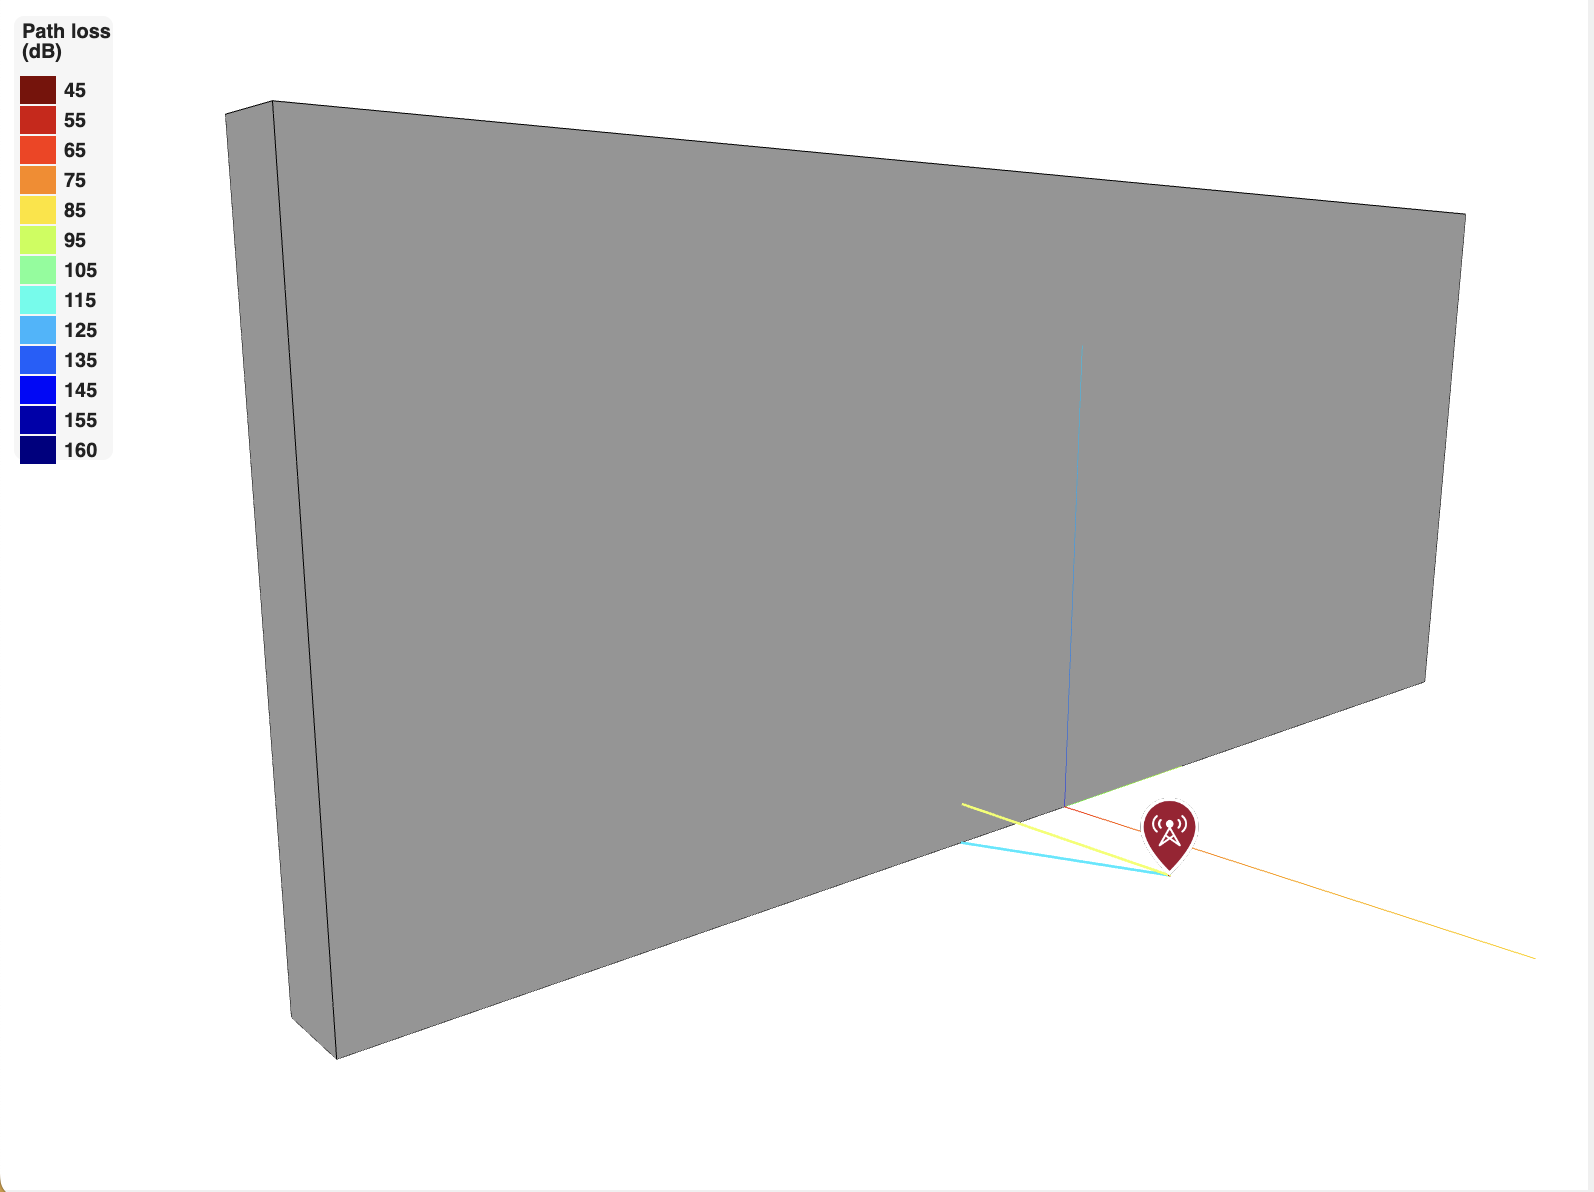
\includegraphics[scale=.3]{figures/check_simulation_left.png}}
    \end{subfigure}
    \begin{subfigure}{0.45\textwidth}
        \centering
        \adjustbox{height=5.2cm}{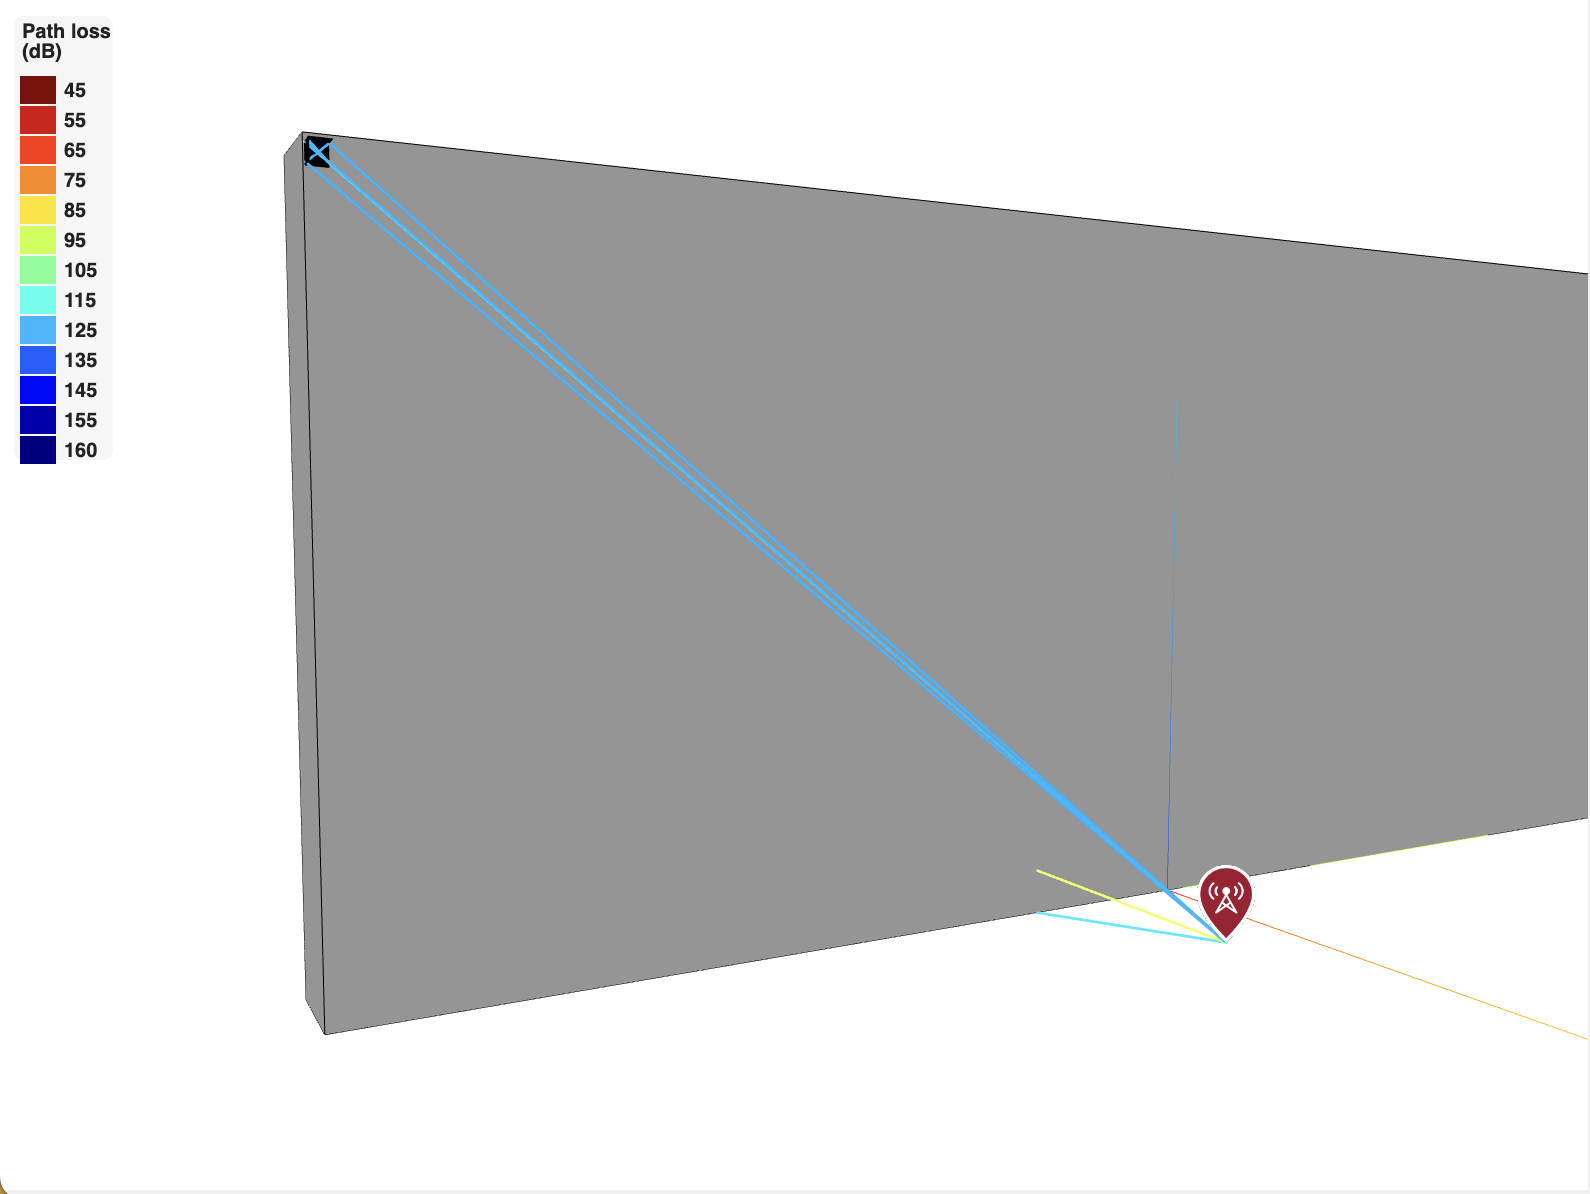
\includegraphics[scale=.3]{figures/check_simulation_reflector.png}}
    \end{subfigure}
    \caption{View of the plausibility check in ray tracing}
    \label{view of the plausibility check in ray tracing}
    \end{figure}
    
\end{enumerate}

In addition, not all rays will be used. According to the observation in all the figures above, two rays always exist and do not have much useful meaning. One is the ray directly transmitted between the transmitter and the receiver, and the other is the ray reflected by the floor under the robot. Since these two rays exist in any case and the range between the transmitter and the reflectors is at least $3\,\mathrm{m}$, a possibility is to get rid of these rays is comparing the propagation distance of rays, such as filtering out when the propagation path is less than 0.1m. Since the antenna height defaults to $0.5\,\mathrm{m}$ but the receiver and the transmitter are quite close but not in the same position, the actual range will not be exact as 0.5m, then we set a range such as $0.45-0.55\,\mathrm{m}$ to filter out the ray reflected by the ground below.

\subsection{Raytracer parameter} \label{Raytracer parameter}
After completing the ray tracing, all the rays will be packaged in a cell, which contains all the properties of the rays. For the above three cases, under the limitation of a maximum of four reflections, one diffraction, and a maximum loss of $150\,\mathrm{dB}$, the number of obtained rays is:

\begin{enumerate}[label=\textbullet]
    \item in empty room: 202 rays,
    \item in the room with reflectors: 701 rays,
    \item in the room with furniture: 1609 rays.
\end{enumerate}

This data confirms the observation above that the amount of received rays does increase with the addition of reflectors and furniture. The properties of the received rays from Matlab \cite{rays_properties} are mainly the following:

\begin{enumerate}[label=\textbullet]
    \item "LineOfSight": The indicator of the LOS information is specified as 0 or 1. The value 1 means the ray has an unobstructed path from the transmitter and receiver, while the value 0 means the ray must have some interactions with other objects.
    \item "Interactions": This property shows the type of the interactions, such as reflection, diffraction, or anything else, as well as the position of the interaction and the name of the material.
    \item "PropagationDelay": The time delay of the propagation path will be specified as a nonnegative value in seconds.
    \item "PropagationDistance": The distance of the propagation will be specified as a nonnegative value in meters.
    \item "AngleOfDeparture": The departure of the angle contains the azimuth angle and elevation angle information of the ray departing from the transmitter, in the form of $[az; el]$
    \item "AngleOfArrival": Similar to the angle of the departure with the form but for the ray arriving at the receiver.
    \item "PathLoss": The path loss is specified as a nonnegative scalar as well in unit dB.
    \item "PhaseShift": The phase shift is specified as a value in radian.
\end{enumerate}

Based on the properties obtained from the ray, some additional points need attention before using them in the radar receive signal computation, namely equation \ref{radar model formula}:

\begin{enumerate}[label=\textbullet]
    \item In the following calculations, we will add an anisotropic radiation pattern and radar cross-section to the rays reflected from the transmitter to the receiver through the reflector once. Hence, it's important to filter these LOS rays out. However, after obtaining the LOS properties, we found that it counts the ray directly from the transmitter to the receiver, so it is not directly applicable to our situation.

    And because the LOS ray between transmitter and receiver has already been filtered out as in the above text, no ray meets this condition when using the LOS function. In addition, since the single reflection in the entire scene does not only occur in the process with reflectors but also can occur only through the wall, another method will be used for finding the LOS rays.

    Since the position of the reflectors in the scene is known, multiple receivers could be directly placed at the position of the reflectors, so that the LOS rays could be found by using the LOS function \cite{los_function} or directly setting the maximum number of reflections and diffractions. The operation and effect of this method will be shown in the next section \ref{Modeling of the radar reflector returns}.

    \item For the propagation distance, since the transmitter and receiver are located on the same platform of the robot in the simulation, the signals propagate a forth-and-back path. In the process of calculating the matrix of the baseband signal, the range refers to the distance between the target point and the radar, so the propagation distance should be divided by 2.

    However, according to the LOS method as mentioned above, that is, setting the receivers directly at the reflectors' position, the signals only propagate one way to the target point, so no division is required.

    \item For the obtained angle of departure and arrival, the difference in angle can be ignored because the interval between the transmitter and the receiver is very small. This angle is critical to the velocity in the radar model because the velocity in the radar model represents the relative speed between the robot and the target point, that is, the vertical component of the velocity on the straight-line. Therefore, the straight-line direction should be calculated according to the angle of departure.

    Figure \ref{conversion between coordinates} illustrates the azimuth and elevation angle. The conversion between the euclidean and spherical coordinates with the angle and range \cite{coordinate_definition} is defined as follows:

    \begin{equation}
    \centering
    x = R\cdot cos(el)\cdot cos(az),
    \end{equation}

    \begin{equation}
    \centering
    y = R\cdot cos(el)\cdot sin(az),
    \end{equation}

    \begin{equation}
    \centering
    z = R\cdot sin(el).
    \end{equation}

    If the range $R$ is set as 1, the range between the robot and the target point will be normalized as a direction. Then the vertical component $v_m$ can be done by a dot product of velocity $v$ and direction $a$, namely

    \begin{equation}
    \centering
    v_m = vcos(\theta) = \frac{\underline{v} \cdot \underline{a}^{T}}{R} = \underline{v} \cdot \underline{a}^{T},
    \end{equation}
    where $\underline{a}$ represents the incident ray in the form of $\underline{a}^{T}=[x, y, z]$.

    \begin{figure}[t]
	\centering
	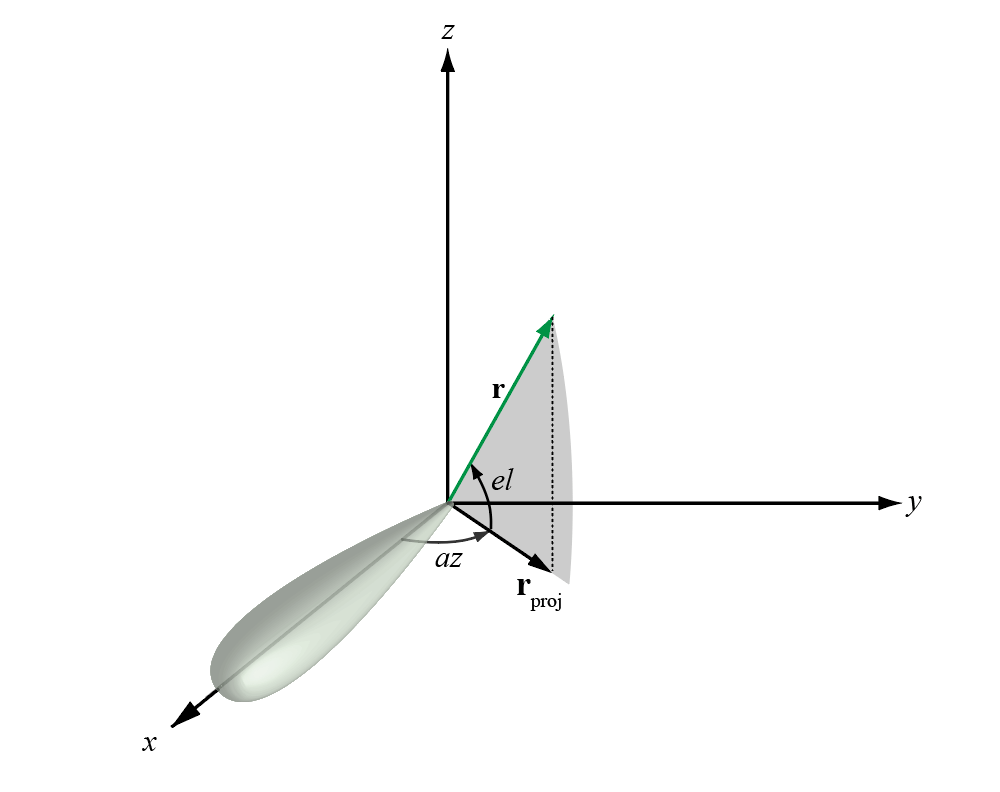
\includegraphics[scale=.4]{figures/relative_velocity.png}
	\caption{Conversion between coordinates \cite{coordinate_definition}}
	\label{conversion between coordinates}
    \end{figure}
    
\end{enumerate}

As all the parameters have been obtained from raytracing, implement them into the radar model, then the Algorithm \ref{radar model pseudo code} can be written as Algorithm \ref{radar model pseudo code detailed} in detail.

\begin{algorithm}[t]
    \caption{Pseudo code of the radar model implemented with parameters}
    \label{radar model pseudo code detailed}
    \renewcommand{\algorithmicrequire}{\textbf{Input:}}
    \renewcommand{\algorithmicensure}{\textbf{Output:}}
    
    \begin{algorithmic}[1]
        \REQUIRE $rays$
        \ENSURE $X\_sum\ as\ sample\ vector$
        
        \STATE $N_s\ =\ 256;$
        \STATE $N_p\ =\ 32;$
        \STATE $X\_sum = zeros(N_s,N_p);$
        \FOR{$m\ =\ 1:length(rays)$}
            \STATE $ray\ =\ rays(m);$
            \STATE $X_k\ =\ zeros(N_s,N_p);$
            \STATE $PL_m\ =\ ray.PathLoss;$
            \STATE $r_m\ =\ ray.PropagationDistance\ /\ 2;$
            \STATE $AoAs\ =\ ray.AngleOfArrival;$
            \STATE $az\ =\ deg2rad(AoAs);$
            \STATE $el\ =\ deg2rad(AoAs);$
            \STATE $a_x\ =\ cos(el) \cdot cos(az);$
            \STATE $a_y\ =\ cos(el) \cdot sin(az);$
            \STATE $a_z\ =\ sin(el);$
            \STATE $a\ =\ [a_x, a_y, a_z];$
            \STATE $v_m\ =\ dot(v, a);$
        
            \FOR{$n_s\ =\ 0:N_s-1$}
                \FOR{$n_p\ =\ 0:N_p-1$}
                    \STATE $P_R\ =\ P_T\ \cdot \ 10^{(-PL_m/10)};$
                    \STATE $A_m\ =\ sqrt(P_R \cdot R);$
                    \STATE $X_k(n_s+1,n_p+1)\ =\ A_m \cdot exp(2j\cdot pi \cdot (2\cdot B \cdot r_m\cdot T_s\cdot n_s/T/c + 2\cdot f\cdot v_m\cdot T_p\cdot n_p/c));$
                \ENDFOR
            \ENDFOR
            \STATE $X\_sum\ =\ X\_sum\ +\ X\_k;$
        \ENDFOR 
        \STATE $P\_noise = 10^{((N_T - 30 + N_F)/10)};$
        \STATE $V\_noise = P\_noise * R;$
        \STATE $n = sqrt(V\_noise/2) * (randn(N_s, N_p) + 1j* randn(N_s, N_p));$
        \STATE $X\_sum = X\_sum + n;$
    \end{algorithmic}   
\end{algorithm}

After obtaining the parameters of the simulation, they can be substituted into the SNR calculation, namely formula \ref{Radar range equation} with the simulated loss rather the theoretical loss to verify whether the required minimum SNR value is achieved. As the required minimum SNR value is still set as $15\,\mathrm{dB}$, and then calculated in Matlab, the minimum required power of the transmitter should be $0.3\,\mathrm{mW}$. The reason for the power difference between this result and the calculation by hand in section \ref{Radar range equation} is that here not only the LOS rays are considered but all the rays in the simulation that has to satisfy the SNR requirement. The loss of other rays is much larger than the value of the LOS rays. According to the hardware of the radar \cite{datasheet}, the maximum power is $5\,\mathrm{mW}$, so it's quite enough for the requirement. Meanwhile, if using the maximum power of the robot, then the SNR would be $27\,\mathrm{dB}$ larger than the expected value.

\section{Modeling of the radar reflector returns} \label{Modeling of the radar reflector returns}
This section will introduce the implementation and results in detail. As mentioned above, in summary, the purpose and problems of LOS are mainly the following:

\begin{enumerate}[label=\textbullet]
    \item The toolchain expects to get the range and relative velocity between the target point and the robot, but the desired targets are mainly the reflectors. And if later we are going to add the anisotropic radiation pattern and radar cross-section into the rays, it's necessary to find out the rays passing through reflectors. That's the first reason for doing this in this section.

    \item The second reason is that there are multiple reflections inside a reflector which makes the path loss so high and can't represent the rays from reflectors well. Therefore, to simulate the strong rays from reflectors well, this section should be done separately.

    \item Another thing is, that there is no suitable property to filter the rays based on the objects in the reflection path and the number of reflections, so we use the tricky method below.
\end{enumerate}

This method is based on the known positions of the reflectors in the scene. Multiple receivers are placed directly at the positions of the reflectors to obtain rays that reach the receiver directly from the transmitter without reflection, which is equivalent to filtering out the rays that are reflected once by the reflectors.

Compared to the ray tracing of the entire scene in the previous section, the simulation here needs the following changes:

\begin{enumerate}[label=\textbullet]
    \item The position of receivers should be modified. In this case, the receiver's position will no longer be a single position but will correspond to the positions of all reflectors. In Matlab, you can directly set a series of the coordinate positions, i.e. $rx\_positions = [[-9.3;-0.7;3.5], [-9.3;-9.3;3.5], [9.3;-9.3;3.5], [9.3;9.3;3.5], [0.7;9.3;3.5]]$. And use this variable $rx\_positions$ directly into the $rxsite$ of ray tracing in Matlab.

    \item In the parameter settings of ray tracing, two parameters need to be modified, namely the maximum number of reflections $MaxNumReflections$ and the maximum number of diffractions $MaxNumDiffractions$, both of which are set to 0.

    \item Due to the uncertainty of the robot's position, it is not possible to guarantee that all reflectors can be observed at any position in the room. Especially in our L-shaped room, if the robot moves to one side of the room, it is very likely that one or two reflectors on the other side will not be visible. Since all receivers are directly placed at the reflector positions, each receiver will get a value. For reflector positions that cannot be seen, the result returned will be an empty set, while visible reflector positions will get a real ray.

    Therefore, it's necessary to filter out the empty set. With the use of the $isempty$ function in Matlab and a loop, the set with valid ray information could be added into a new cell and passed to the radar model. In Figure \ref{view of non LOS rays} it can be seen the meaning of non-line-of-sight rays.
    
\end{enumerate}

After passing the newly obtained rays to the radar model, there will be some differences in the properties of the rays compared to the previous processing method, mainly including the following points:

\begin{enumerate}[label=\textbullet]
    \item In the previous section, since the transmitter and receiver are both packaged on the same platform of the robot, each ray has a round trip during the propagation process. But the range refers to the relative distance between the robot and the target point, so the propagation path should be halved. However, for the newly obtained rays, the propagation distance does not need to be halved and can be used directly.

    \item Since the reflectors are bypassed during this simulation, the loss information will be inaccurate. Considering the addition of the anisotropic patterns later, the path loss information for this part of the LOS rays will be calculated by hand using the formula \ref{Radar range equation} while the propagation distance still uses the simulated propagation distance.

    \item The manually calculated losses of LOS rays have a negative sign. Note the change in sign when mixed with the simulated rays from the previous section in the radar model.

    \item As mentioned in the previous section, the tiny difference between the AoD and AoA can be neglected. However, in the current situation, since the transmitter and receiver are no longer on the same platform, the two angles cannot be confused. The AoD, i.e. the angle of ray leaving the transmitter, will be used as the determining factor for the subsequent radiation pattern, while the AoA, i.e. the angle of ray arriving the receiver, will determine the value of the radar cross-section.
\end{enumerate}

Figure \ref{view of LOS rays} demonstrates the effect of the LOS rays where there are two cases, on the left side in the case of five reflectors, while on the right side with more reflectors. The effect of more reflectors on the range Doppler map will be tested as well, so it's necessary to simulate it here. As mentioned above, if the robot is on one side of the L-shaped room, the reflectors on the other side are likely NLOS. Figure \ref{view of non LOS rays} illustrates the situation for that.

\begin{figure}[t]
    \centering
    \begin{subfigure}{0.45\textwidth}
        \centering
        \adjustbox{height=5.2cm}{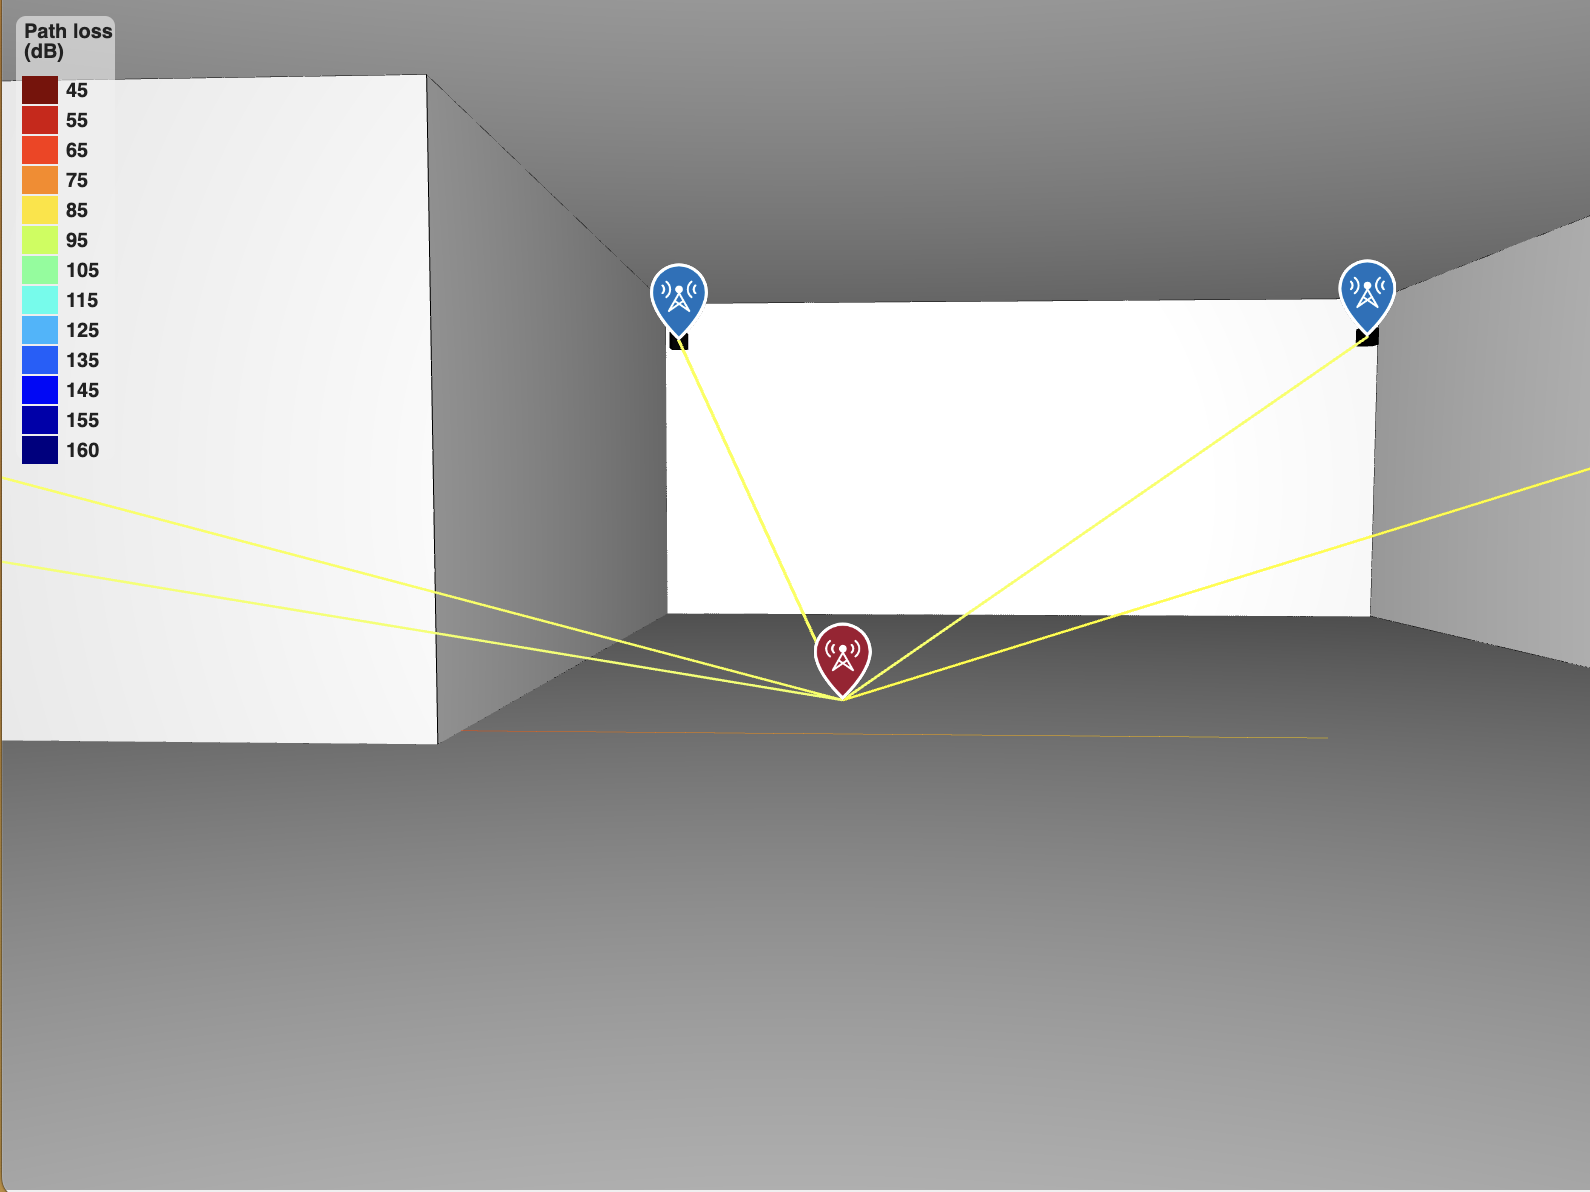
\includegraphics[scale=.3]{figures/LOS_5_reflectors.png}}
    \end{subfigure}
    \begin{subfigure}{0.45\textwidth}
        \centering
        \adjustbox{height=5.2cm}{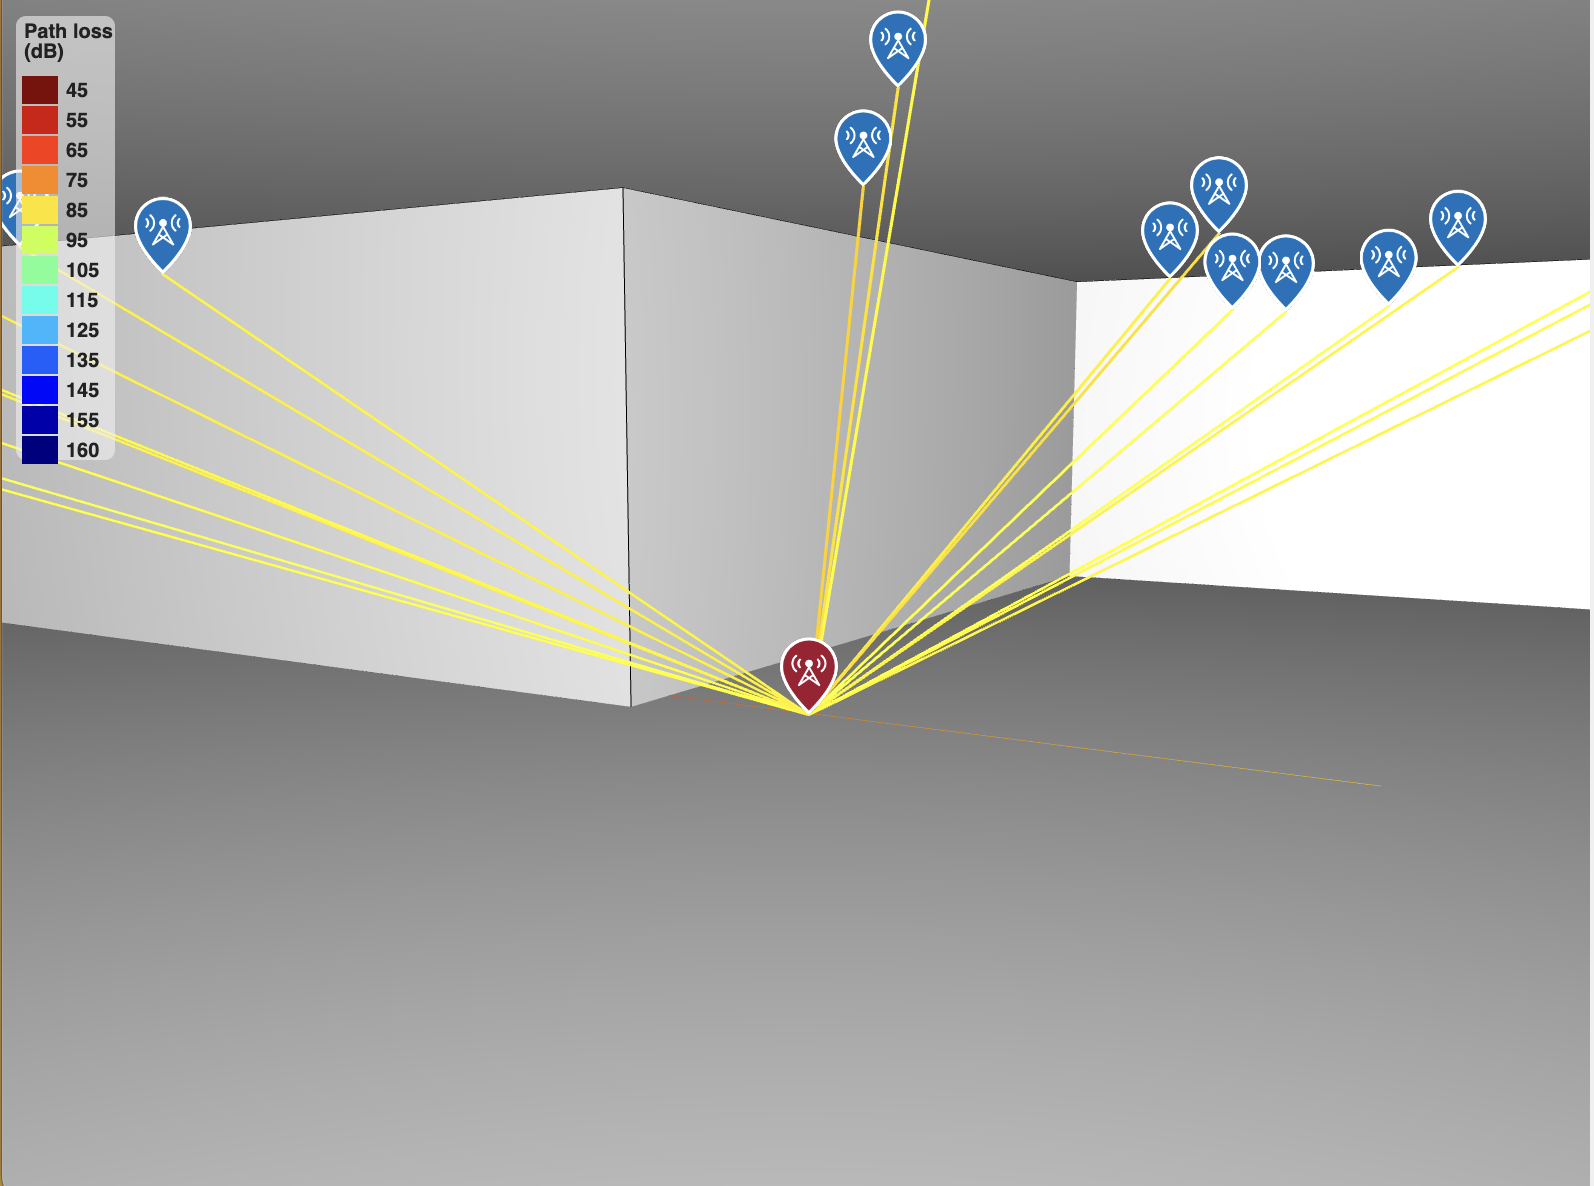
\includegraphics[scale=.3]{figures/LOS_more_reflectors.png}}
    \end{subfigure}
    \caption{View of LOS rays, left one with 5 reflectors while right image with more reflectors.}
    \label{view of LOS rays}
\end{figure}

\begin{figure}[t]
	\centering
	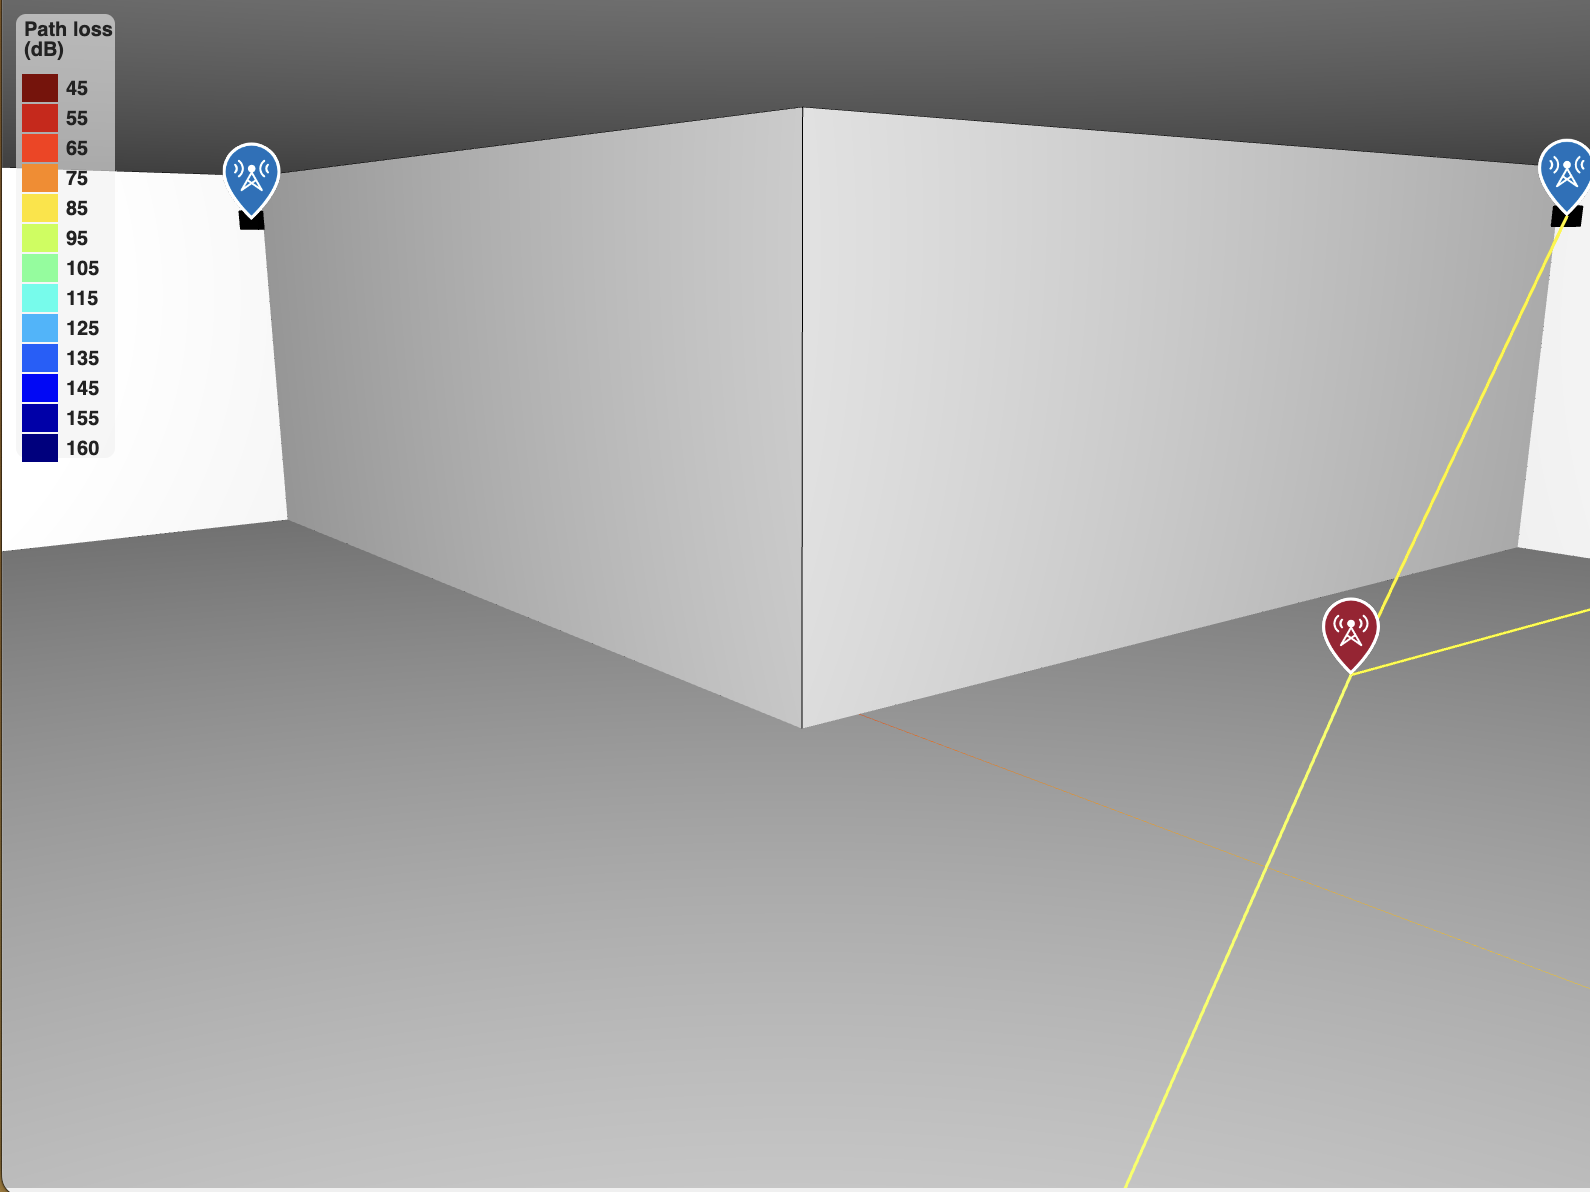
\includegraphics[scale=.3]{figures/LOS_with_empty_set.png}
	\caption{The reflector without LOS ray}
	\label{view of non LOS rays}
\end{figure}

Figure \ref{view of LOS rays with furniture} illustrates the view of the LOS rays with furniture. Due to the uncertainty of the position and height of furniture, and the robot is relatively lower, the LOS rays may be blocked. Figure \ref{view of the blocking ray by furniture} shows the view of the blocking ray as the robot stands in the same position. It can also be pointed out that in the subsequent signal processing and range-Doppler map, the foreseeable impact of furniture, in addition to the strong signal caused by being too close to the object, may be the occlusion of previously visible LRPs.

\begin{figure}[t]
    \centering
    \begin{subfigure}{0.45\textwidth}
        \centering
        \adjustbox{height=5.2cm}{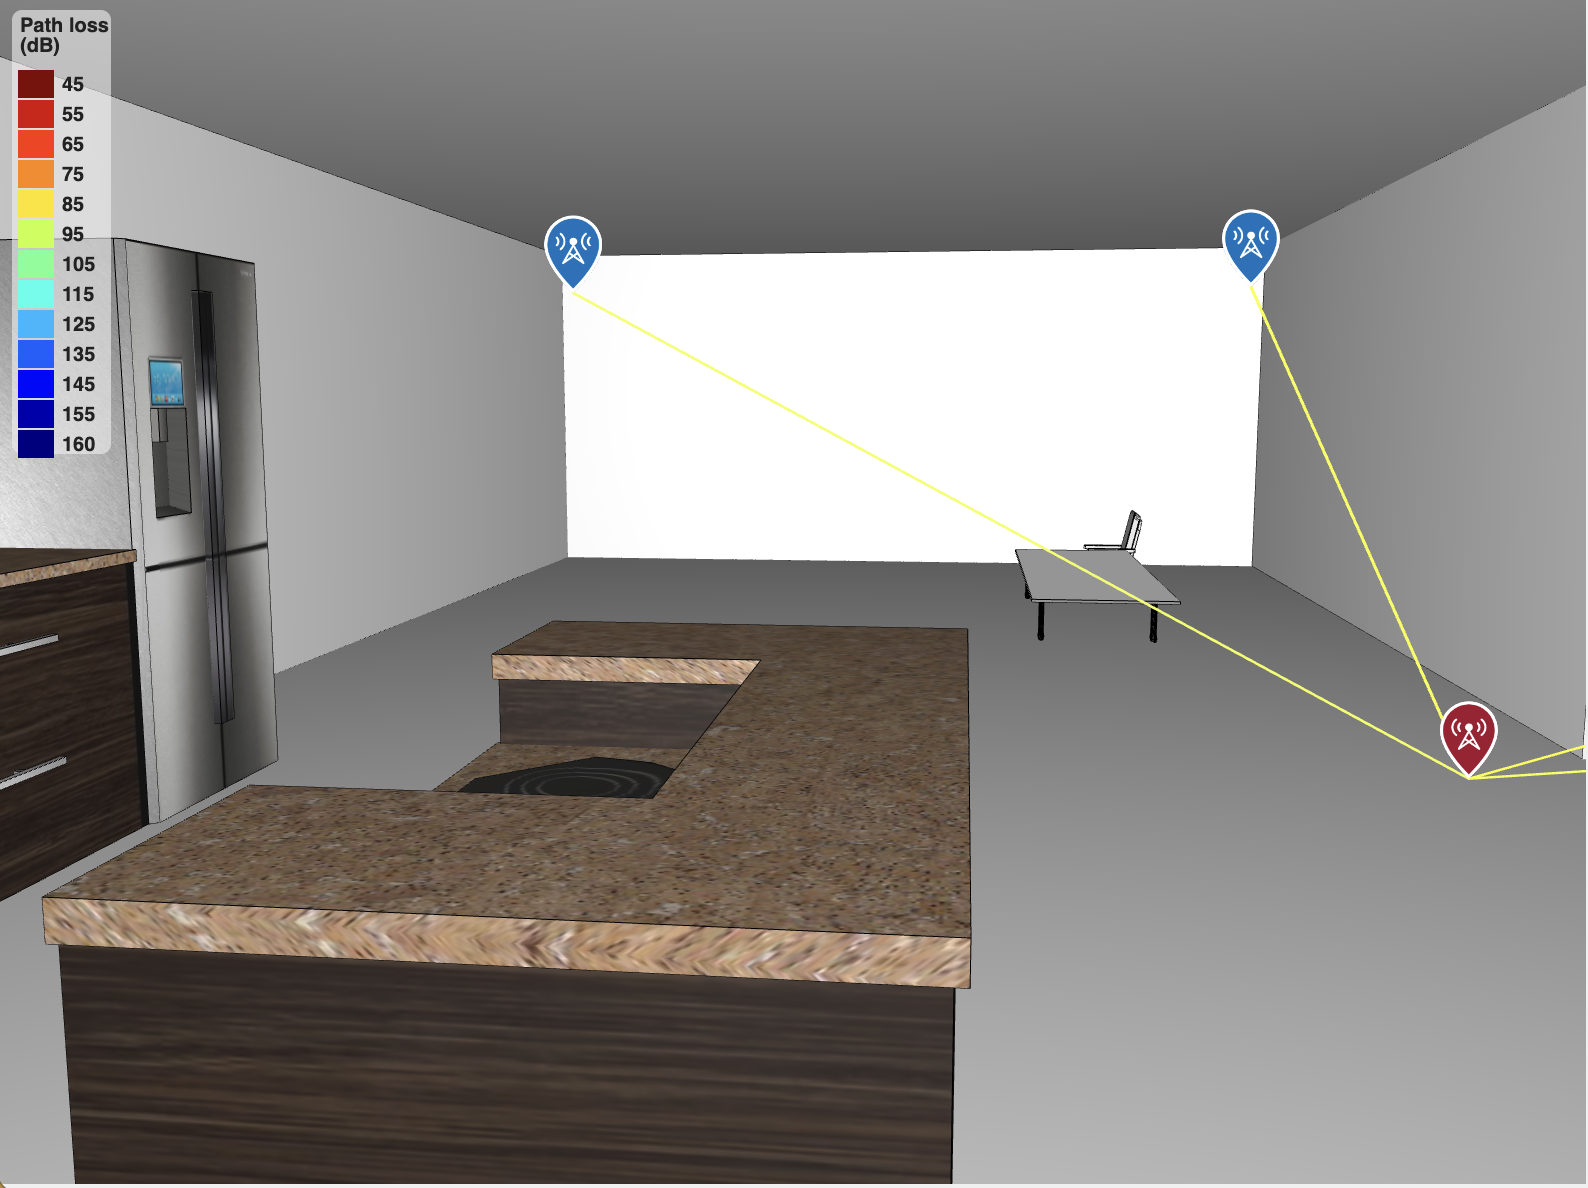
\includegraphics[scale=.3]{figures/LOS_furniture_left.png}}
    \end{subfigure}
    \begin{subfigure}{0.45\textwidth}
        \centering
        \adjustbox{height=5.2cm}{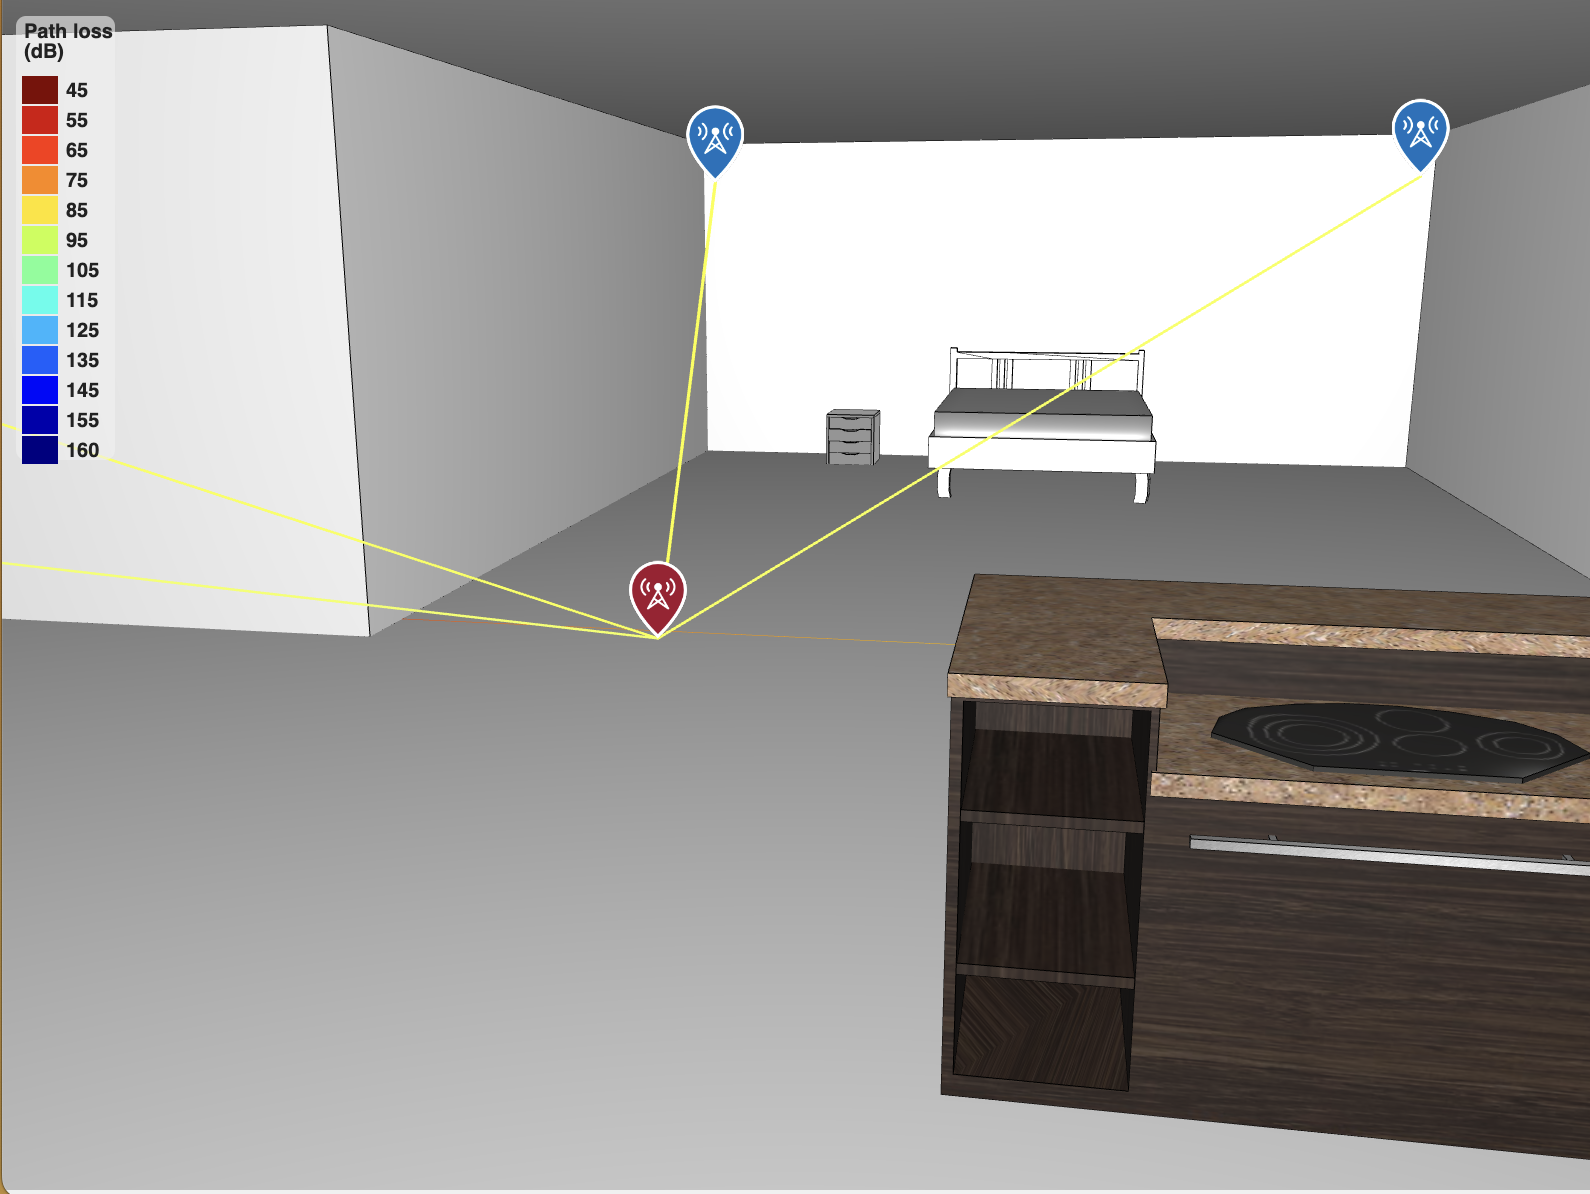
\includegraphics[scale=.3]{figures/LOS_furniture_right.png}}
    \end{subfigure}
    \caption{View of LOS rays with furniture}
    \label{view of LOS rays with furniture}
\end{figure}

\begin{figure}[t]
    \centering
    \begin{subfigure}{0.45\textwidth}
        \centering
        \adjustbox{height=5.2cm}{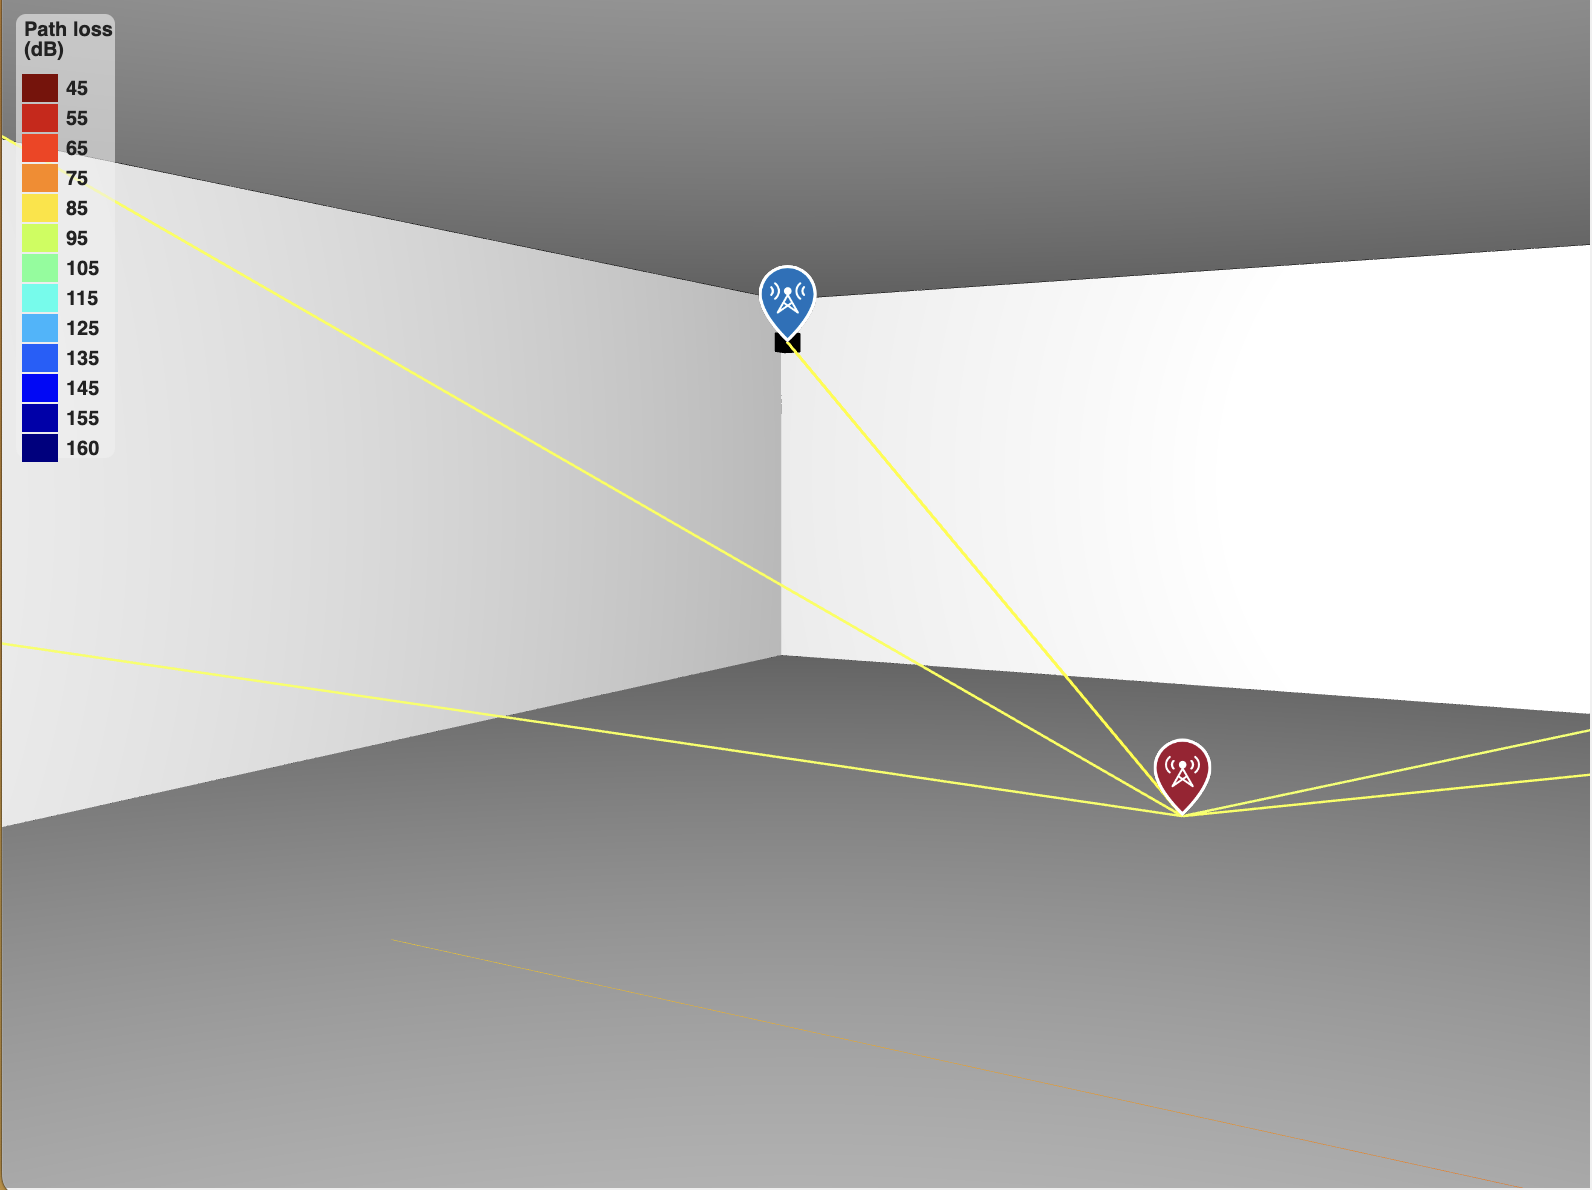
\includegraphics[scale=.3]{figures/LOS_empty_room_back.png}}
    \end{subfigure}
    \begin{subfigure}{0.45\textwidth}
        \centering
        \adjustbox{height=5.2cm}{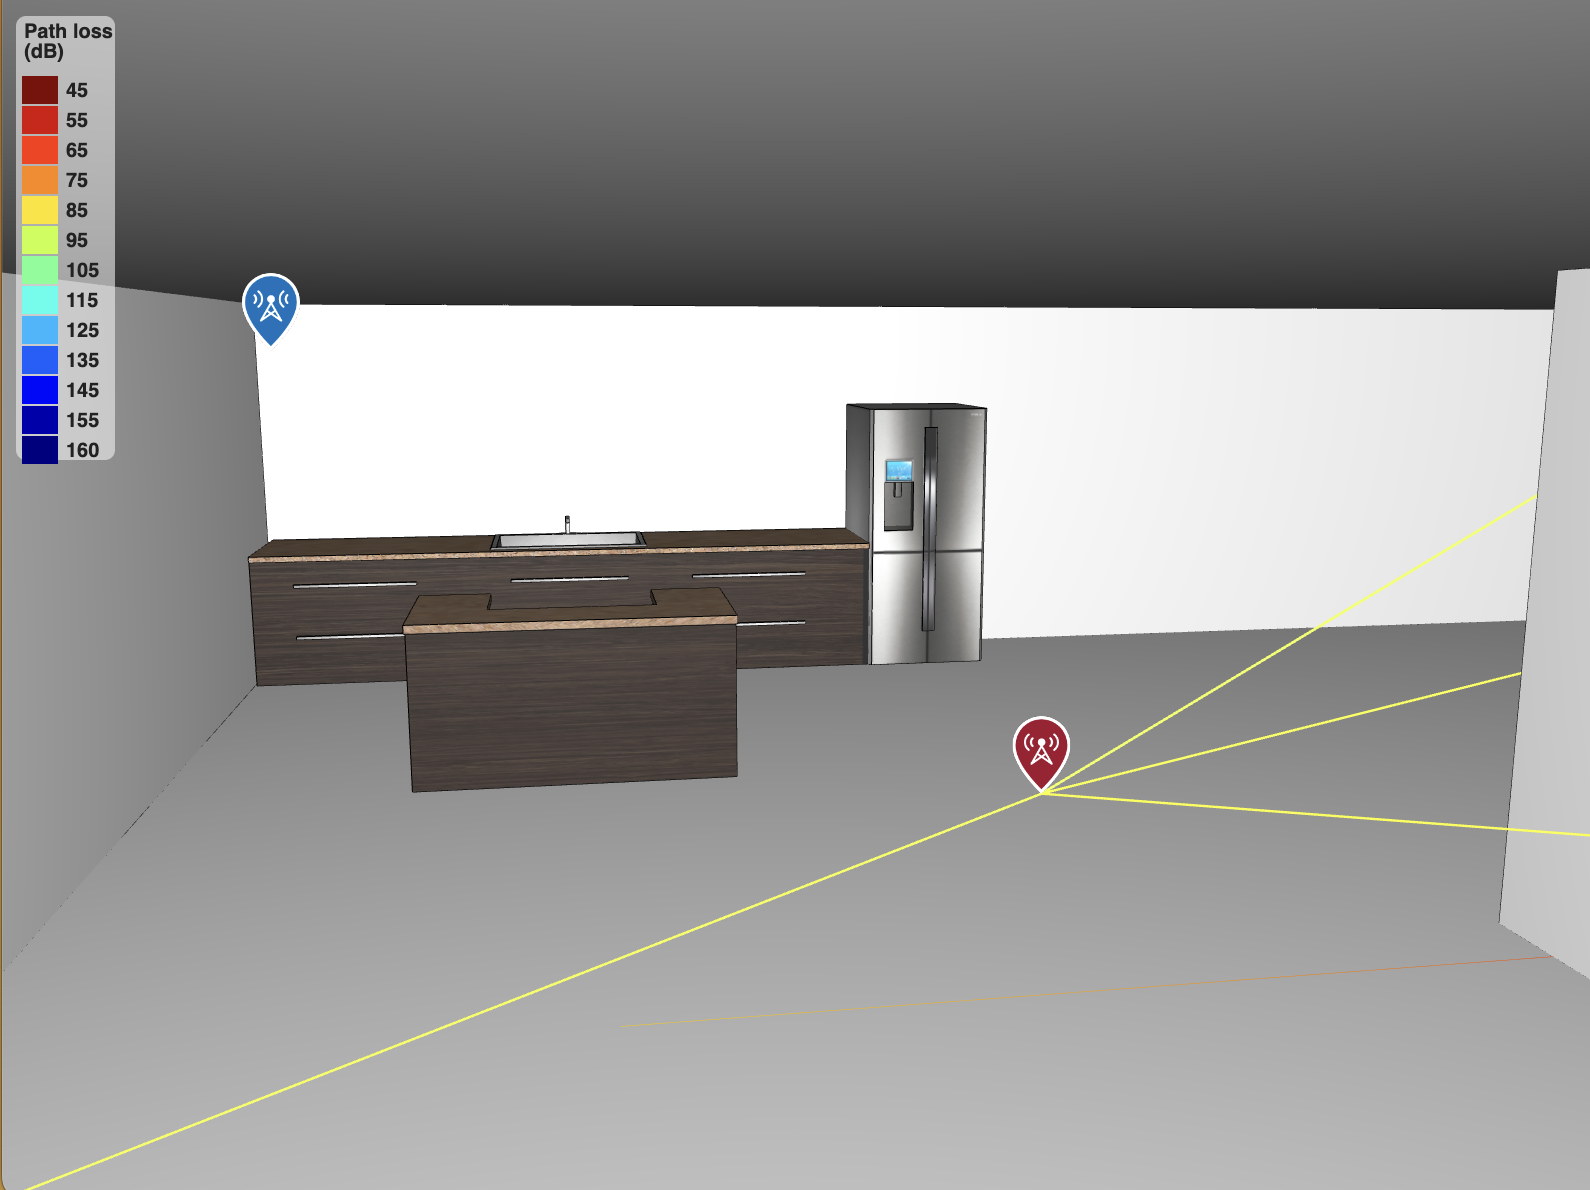
\includegraphics[scale=.3]{figures/LOS_furniture_back.png}}
    \end{subfigure}
    \caption{View of the blocking ray by furniture}
    \label{view of the blocking ray by furniture}
\end{figure}

\section{Antenna radiation pattern} \label{Antenna radiation pattern}
In this section, an antenna will be designed in Matlab based on the parameters of the real antenna, and the anisotropic radiation pattern will be obtained according to different angles and added to the current simulation.

\begin{spacing}{1.5}
\textbf{\large{Antenna Designer}}
\end{spacing}

The designed antenna is based on Infineon's type BGT60TR13C product \cite{datasheet}. The design is performed in Matlab regarding its package size, gain, and angle parameters. Figure \ref{size of the antenna package} illustrates the size of the antenna package where the top image shows the size of the whole package and the bottom one illustrates the interval between multiple antennas.

This product contains three receivers and one transmitter, but in our radar system, only one single transmitter and single receiver are needed. However, the size of each antenna can still be designed according to the approximate size of the product itself. At the same time, the interval between the transmitter and the receiver in the radar is very close, as shown in the figure, which is the reason that the distance between the two is set to only $1\,\mathrm{mm}$ in the previous section.

\begin{figure}[!htb]
    \centering
    \begin{subfigure}[b]{\textwidth}
        \centering
        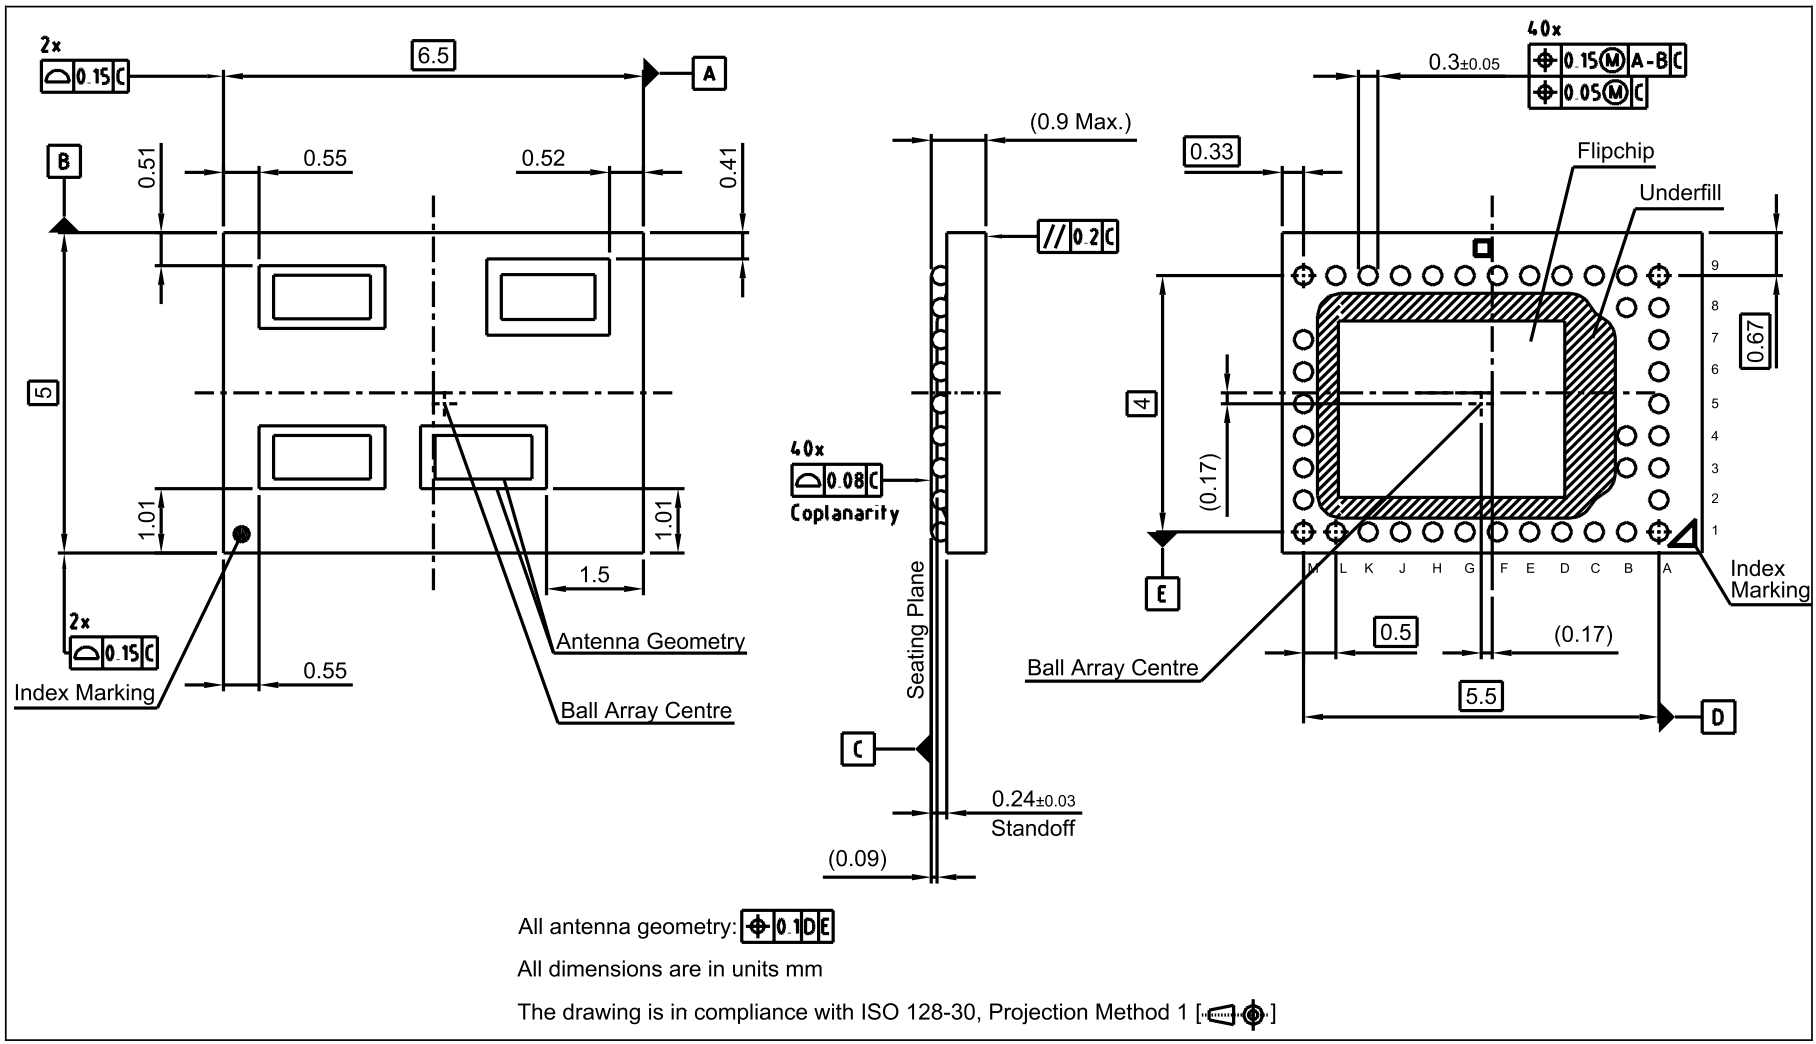
\includegraphics[scale=.48]{figures/size_of_package.png}
        \caption{Size of the whole package}
        \label{size of the whole package}
    \end{subfigure}
    
    \begin{subfigure}[b]{\textwidth}
        \centering
        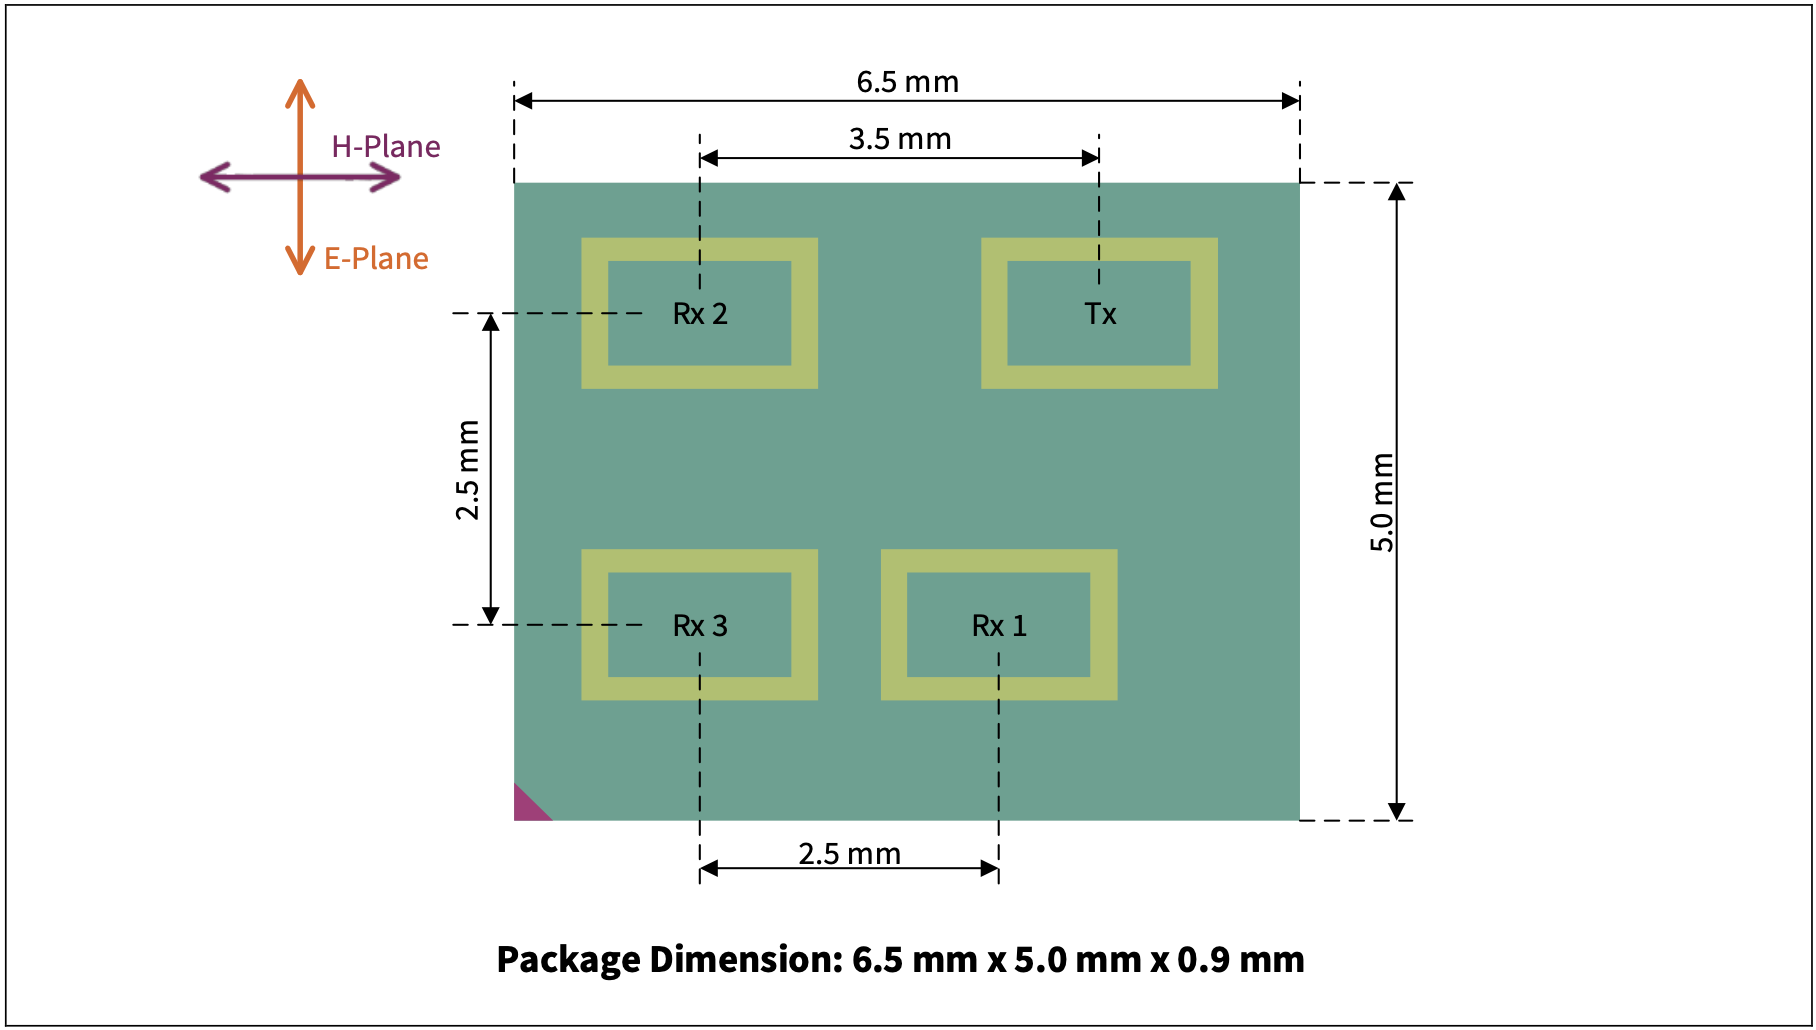
\includegraphics[scale=.48]{figures/size_of_antenna_interval.png}
        \caption{Size of the antennas interval}
        \label{size of the antennas interval}
    \end{subfigure}
    
    \caption{Size of the antenna package \cite{datasheet}}
    \label{size of the antenna package}
\end{figure}

If assumed that in this package, all four antennas are the same size, then the length and width of a single antenna are roughly,
\begin{equation}
    \centering
    length = 6.5\,\mathrm{mm} - 3.5\,\mathrm{mm} - 0.56\,\mathrm{mm} - 0.52\,\mathrm{mm} = 1.93\,\mathrm{mm},
\end{equation}

\begin{equation}
    \centering
    width = 5.0\,\mathrm{mm} - 2.5\,\mathrm{mm} - 0.51\,\mathrm{mm} - 1.01\,\mathrm{mm} = 0.98\,\mathrm{mm}.
\end{equation}
Since this size is obtained based on assumptions and many other antenna specifications need to be achieved, the size of the antenna is set firstly within a certain range to facilitate subsequent adjustments, namely the length in $1.8-2\,\mathrm{mm}$ and the width in the range $0.9-1.2\,\mathrm{mm}$.

Table \ref{specification of the real antenna} \cite{datasheet} demonstrates some other specifications of the real antenna. The frequency of our radar system is determined as $60\,\mathrm{GHz}$ in the range of $58.0-63.5\,\mathrm{GHz}$. As seen in the table, the parameters of the transmitter and receiver are quite similar, so we assume that they are the same in the Matlab designer, and then just design one type for both. The max gain is going to be around $3.5\,\mathrm{dBi}$ and the half-power beam width of a single antenna is assumed as around 60 degrees.

\begin{table}
    \centering
    \caption{Specifications of the real antenna \cite{datasheet}}
    \label{specification of the real antenna}
    \begin{tabular}{lccccc{1cm}}
        \hline
        \multicolumn{1}{l|}{\textbf{Spec}} & \multicolumn{1}{c|}{\textbf{Unit}} & \multicolumn{3}{c|}{\textbf{Value}} & \multicolumn{1}{c}{\textbf{Condition}}\\
        \hline

        \multicolumn{1}{l|}{Parameters} & \multicolumn{1}{c|}{} & \multicolumn{1}{c|}{Min} & \multicolumn{1}{c|}{Typ} & \multicolumn{1}{c|}{Max} & \multicolumn{1}{c}{}\\
        \hline

        \multicolumn{1}{l|}{RX\_BW, TX\_BW} & \multicolumn{1}{c|}{GHz} & \multicolumn{1}{c|}{58.0} & \multicolumn{1}{c|}{} & \multicolumn{1}{c|}{63.5} & \multicolumn{1}{c}{Antenna bandwidth}\\
        \hline

        \multicolumn{1}{l|}{GTX} & \multicolumn{1}{c|}{dBi} & \multicolumn{1}{c|}{2.0} & \multicolumn{1}{c|}{3.5} & \multicolumn{1}{c|}{5.0} & \multicolumn{1}{c}{Antenna gain of a single TX antenna}\\
        \hline

        \multicolumn{1}{l|}{GRX} & \multicolumn{1}{c|}{dBi} & \multicolumn{1}{c|}{2.0} & \multicolumn{1}{c|}{3.5} & \multicolumn{1}{c|}{5.0} & \multicolumn{1}{c}{Antenna gain of a single RX antenna}\\
        \hline

        \multicolumn{1}{l|}{HPBW\_RX\_E} & \multicolumn{1}{c|}{Deg} & \multicolumn{1}{c|}{50} & \multicolumn{1}{c|}{65} & \multicolumn{1}{c|}{80} & \multicolumn{1}{c}{\makecell{Half-power beam width of a single RX \\ antenna in the E-plane direction}}\\
        \hline

        \multicolumn{1}{l|}{HPBW\_RX\_H} & \multicolumn{1}{c|}{Deg} & \multicolumn{1}{c|}{20} & \multicolumn{1}{c|}{35} & \multicolumn{1}{c|}{50} & \multicolumn{1}{c}{\makecell{Half-power beam width of a single RX \\ antenna in the H-plane direction}}\\
        \hline

        \multicolumn{1}{l|}{HPBW\_TX\_E} & \multicolumn{1}{c|}{Deg} & \multicolumn{1}{c|}{50} & \multicolumn{1}{c|}{65} & \multicolumn{1}{c|}{80} & \multicolumn{1}{c}{\makecell{Half-power beam width of a single TX \\ antenna in the E-plane direction}}\\
        \hline

        \multicolumn{1}{l|}{HPBW\_TX\_H} & \multicolumn{1}{c|}{Deg} & \multicolumn{1}{c|}{25} & \multicolumn{1}{c|}{40} & \multicolumn{1}{c|}{55} & \multicolumn{1}{c}{\makecell{Half-power beam width of a single RX \\ antenna in the H-plane direction}}\\
        \hline
    \end{tabular}
\end{table}

There is an app called Antenna Designer in Matlab \cite{antenna_designer_operation}, where you can set various parameters and test whether the antenna satisfy the requirement. Since many parameters do not have an exact value but are within a range, another optimization function offered in Designer \cite{optimization_operation} is necessary, in which you can set the range of parameters and limit the goal according to the required maximum gain to ensure that the parameters permutation and combination in the optimization process are towards the required maximum gain.

The type of antenna is chosen as microstrip which consists of the ground plane, dielectric substrate, patch, and feed line. Therefore, the parameters that need to be set include the overall size of the antenna object, the length and width of the ground plane, the thickness of the substrate, the offset of the patch center, the offset of the feed point, and the characteristics of the conductive medium, etc. Figure \ref{optimization interface} demonstrates the look of the optimization interface and the range of the parameters in the setting.

\begin{figure}[t]
	\centering
	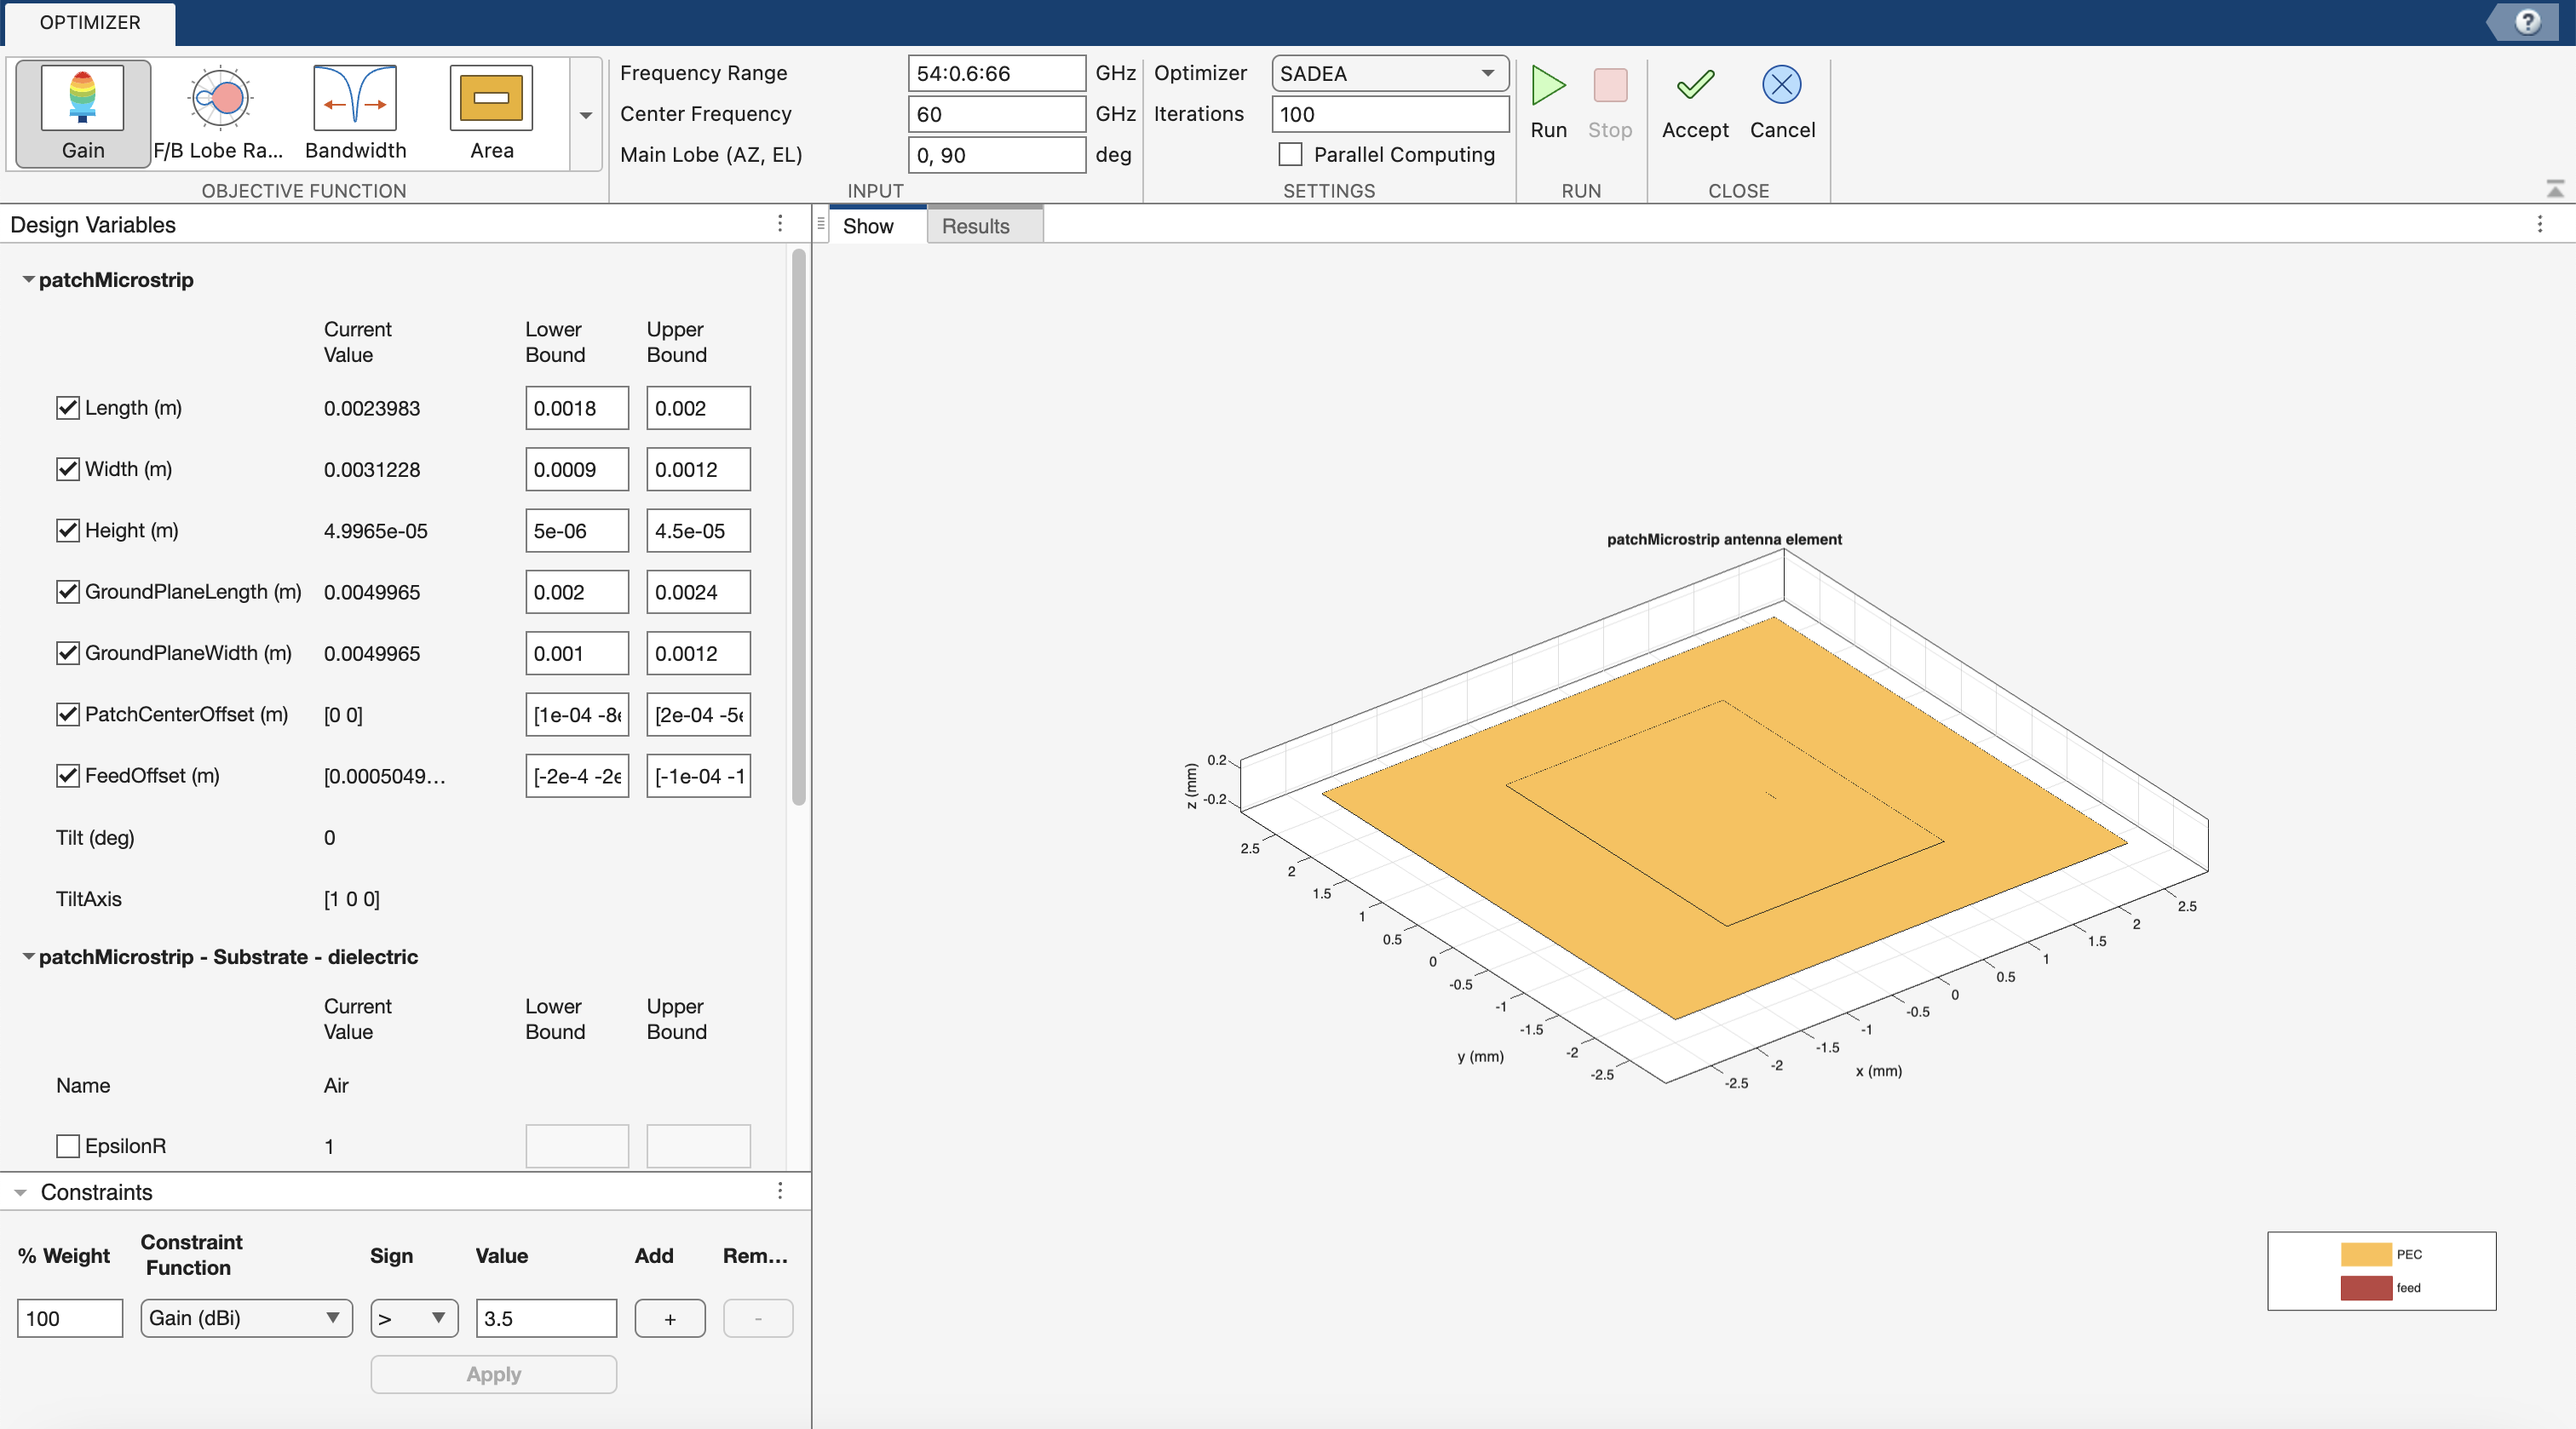
\includegraphics[scale=.28]{figures/optimization_interface.png}
	\caption{Optimization interface and setting range of parameters}
	\label{optimization interface}
\end{figure}

This optimization function can display the values of the target parameters at each moment and generate relevant images. Figure \ref{optimization max gain} shows the changes in the maximum gain parameter during the process. It can be seen that after 50 iterations most of the max gains approach the requirement. The latest iteration could be chosen to apply to the ray tracing simulation. Figure \ref{radiation pattern of antenna after optimization} illustrates the radiation pattern of the generated antenna, where the left one is the pattern in 3D view while the right one is in the elevation view. As checked, the max gain is $4.4\,\mathrm{dBi}$ within the specification and the half power beam width (HPBW) is around 85 degrees above the max 80 degrees but not too much. But this antenna is not finished yet and needs some more updates.

\begin{figure}
	\centering
	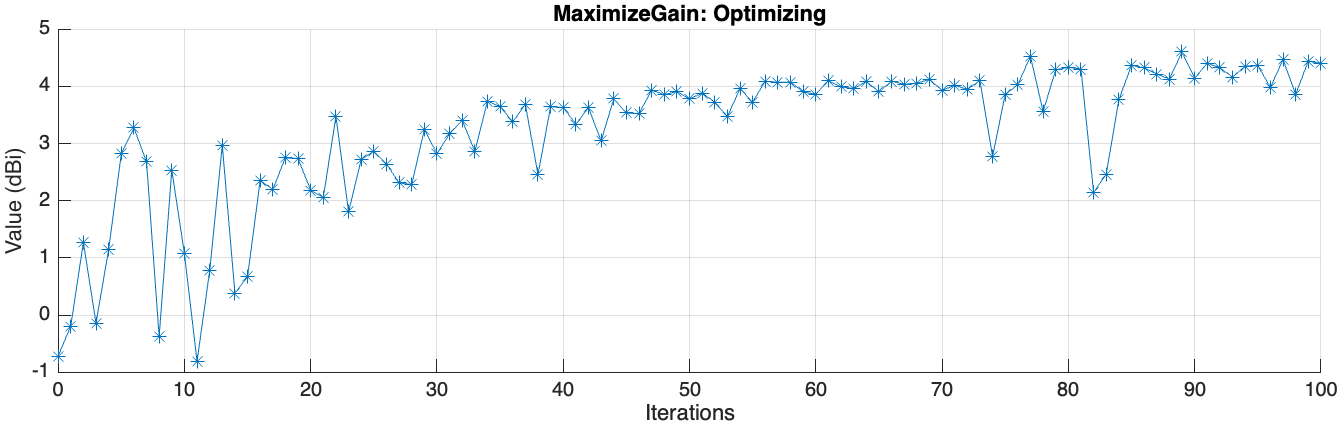
\includegraphics[scale=.68]{figures/optimization_max_gain.png}
	\caption{Max gain during the optimization process}
	\label{optimization max gain}
\end{figure}

\begin{figure}[!htb]
    \centering
    \begin{subfigure}{0.45\textwidth}
        \centering
        \adjustbox{height=6.3cm}{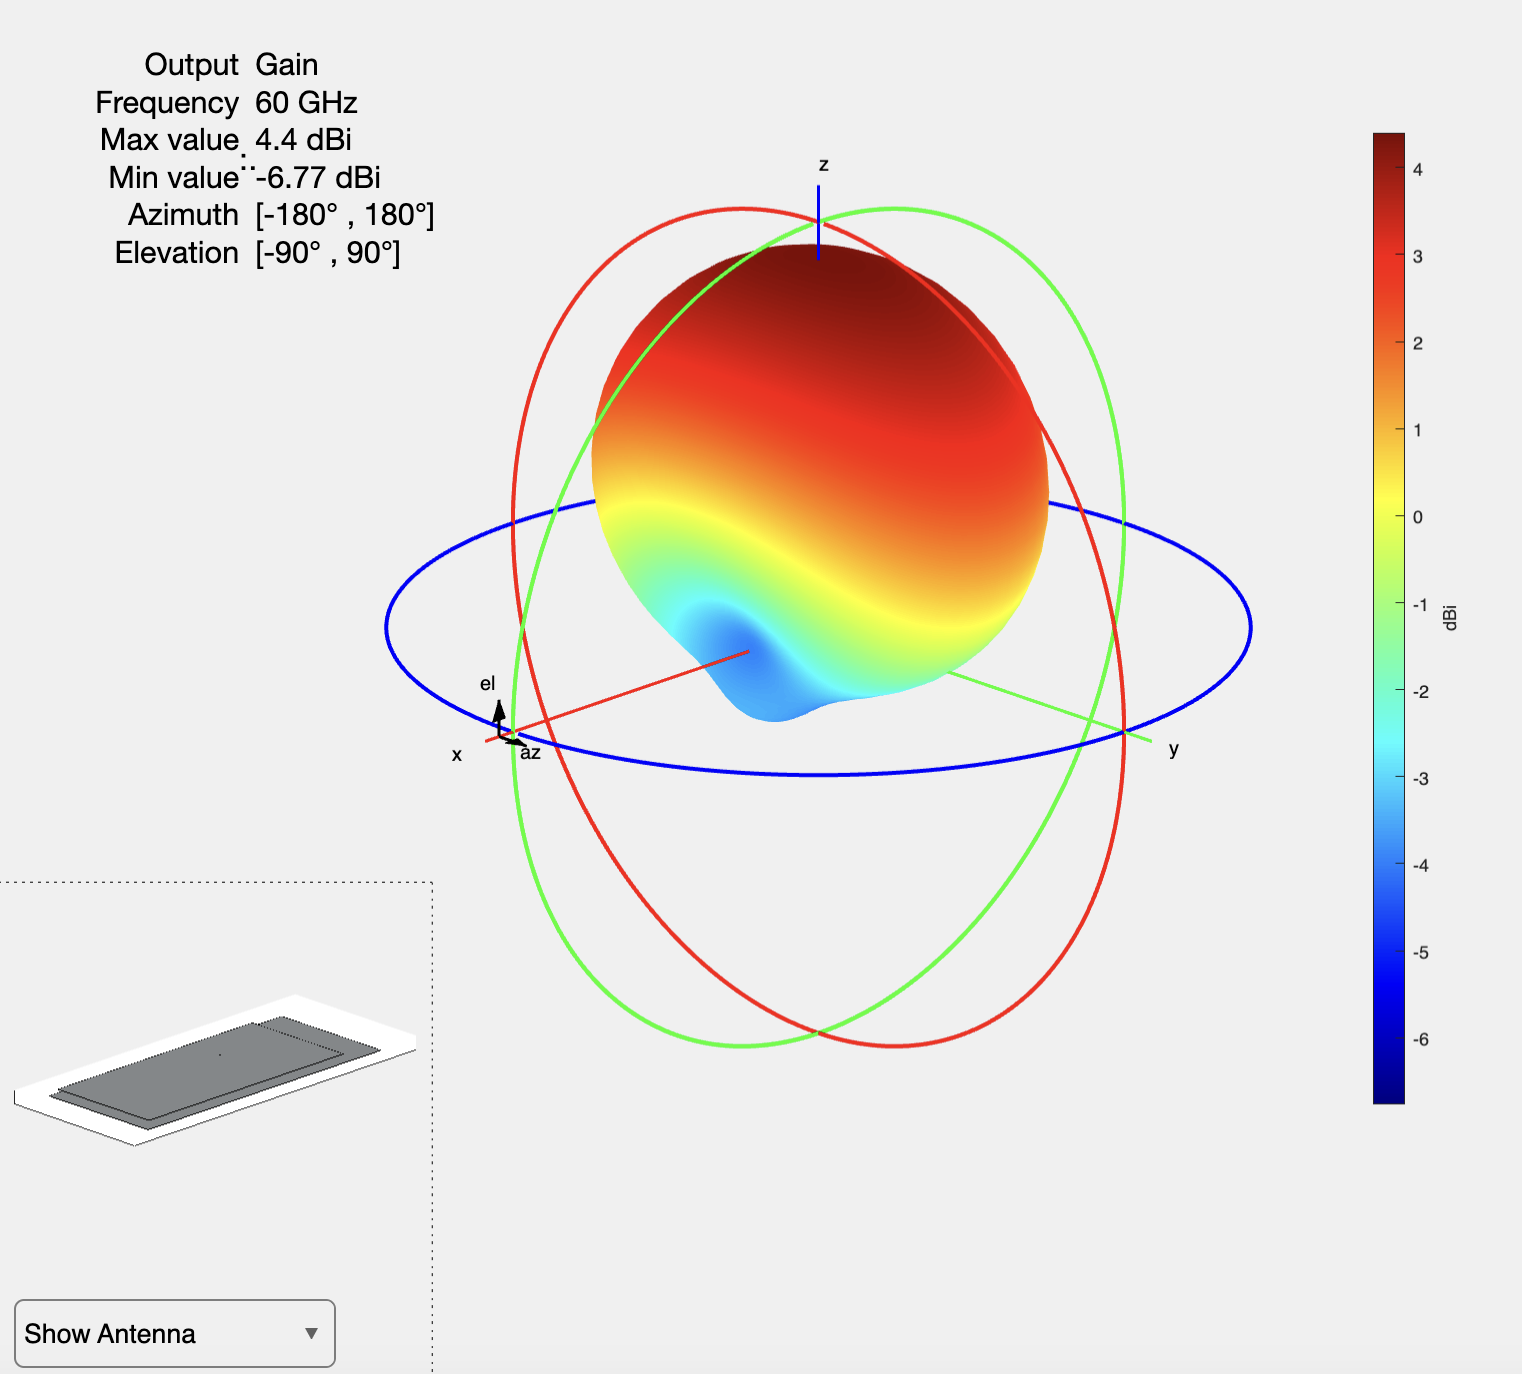
\includegraphics[scale=.3]{figures/radiation_pattern_1version.png}}
    \end{subfigure}
    \begin{subfigure}{0.45\textwidth}
        \centering
        \adjustbox{height=6.3cm}{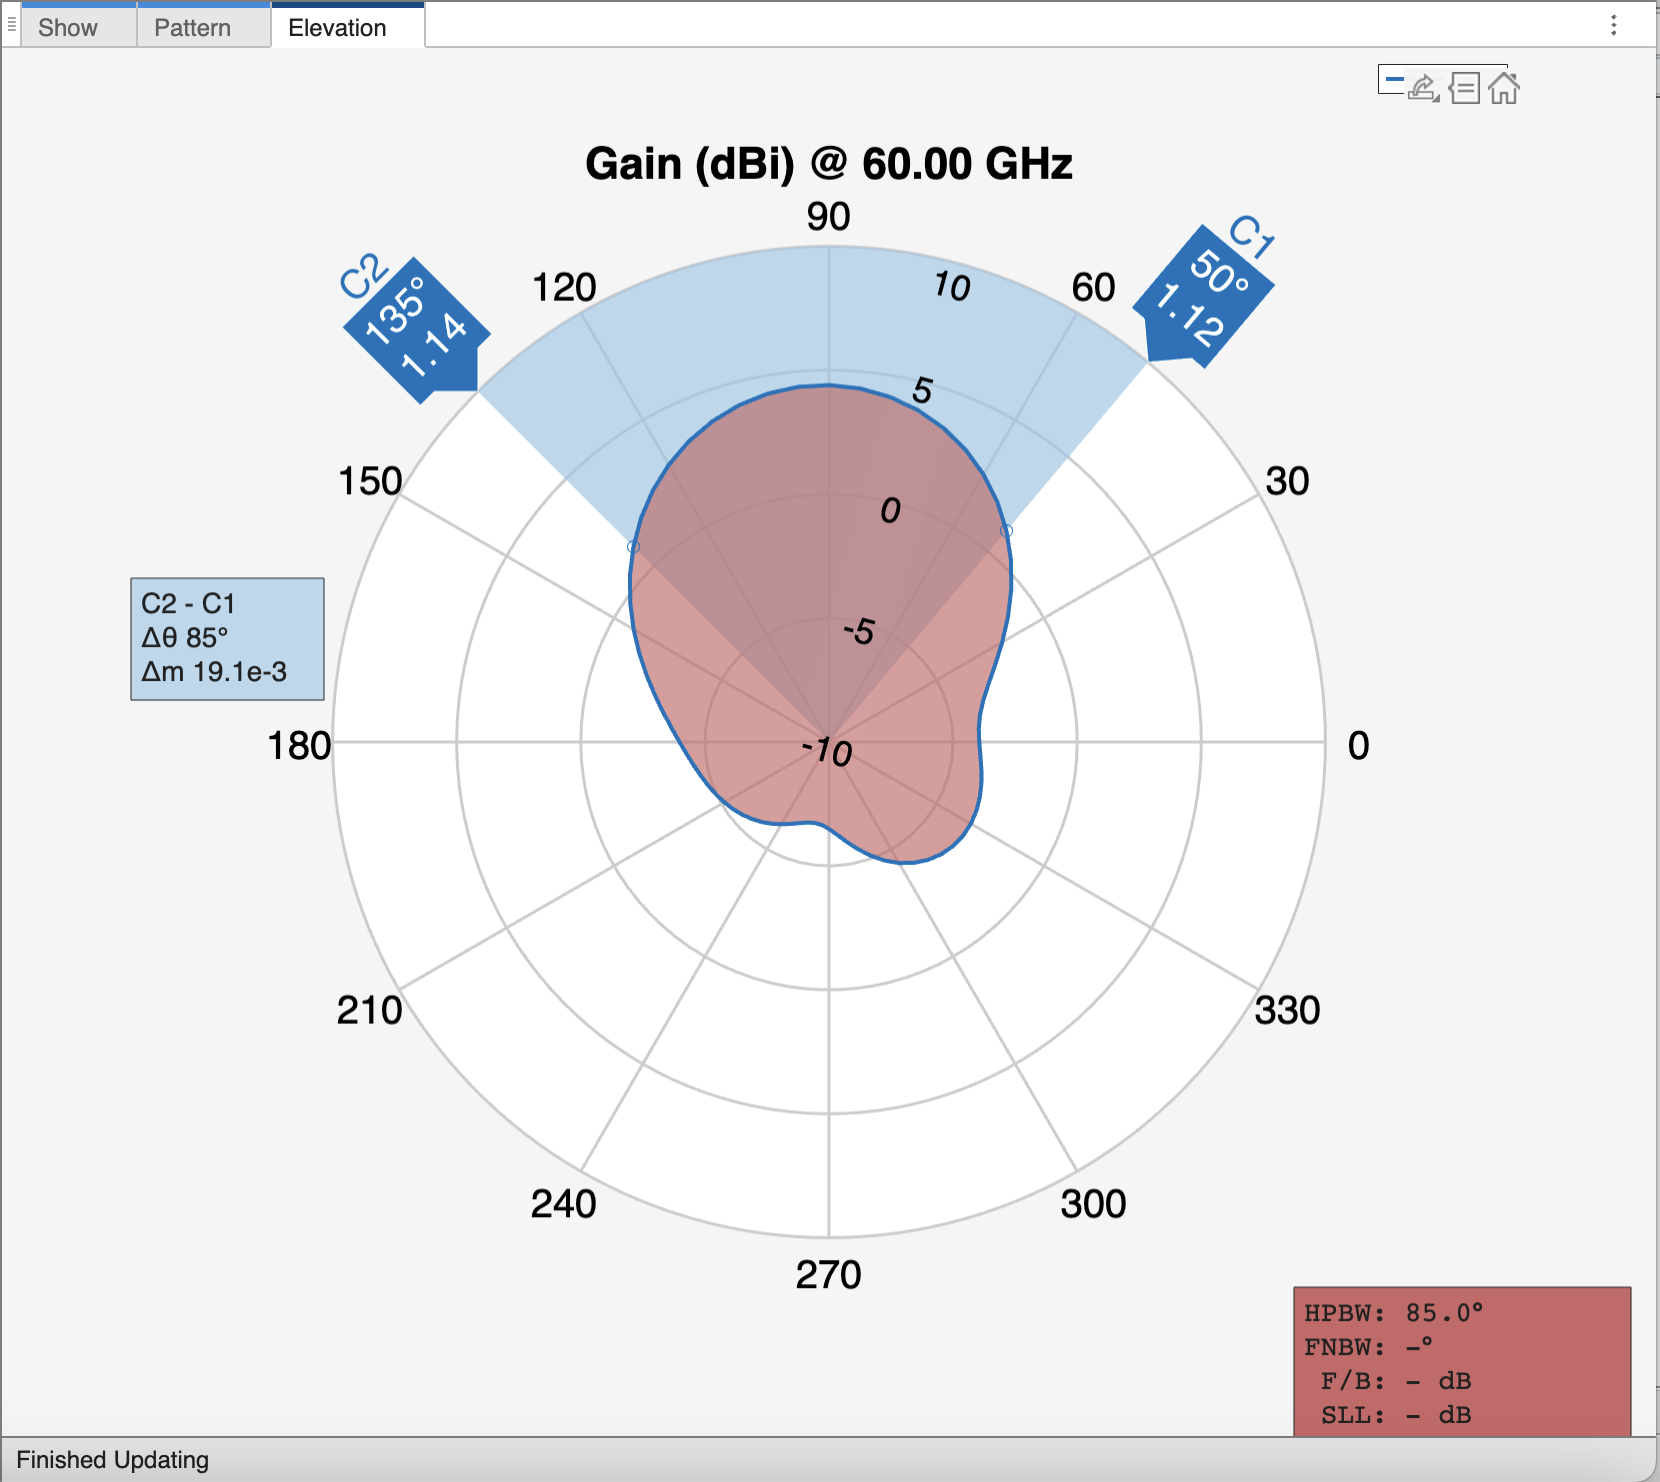
\includegraphics[scale=.3]{figures/radiation_elevation_pattern_1version.png}}
    \end{subfigure}
    \caption{Radiation pattern of antenna after optimization}
    \label{radiation pattern of antenna after optimization}
\end{figure}

As mentioned above, it's better to use a directional antenna. Since we want to get more information about the reflectors, the signal should be more toward the top rather than the surrounding objects. Therefore, after basically satisfying these specifications, we will check the gain of the optimized antenna in each elevation angle in the EH plane, especially the difference between the gain upward and the gain around, which is illustrated in Figure \ref{antenna gain of the previous version}. As seen, the gain is not quite directional, the gain between the horizontal and upper direction is not significantly different, so the parameters have to be manually fine-tuned within a small range. The ideal radiation pattern of this Infineon antenna looks like the Figure \ref{radiation pattern of the Infineon product}. Figure \ref{antenna gain of the final version} shows what the final antenna adjustment looks like. The antenna gain upward and around can be well distinguished, which is close to our expectations.

\begin{figure}[t]
    \centering
    \begin{subfigure}{0.45\textwidth}
        \centering
        \adjustbox{height=4cm}{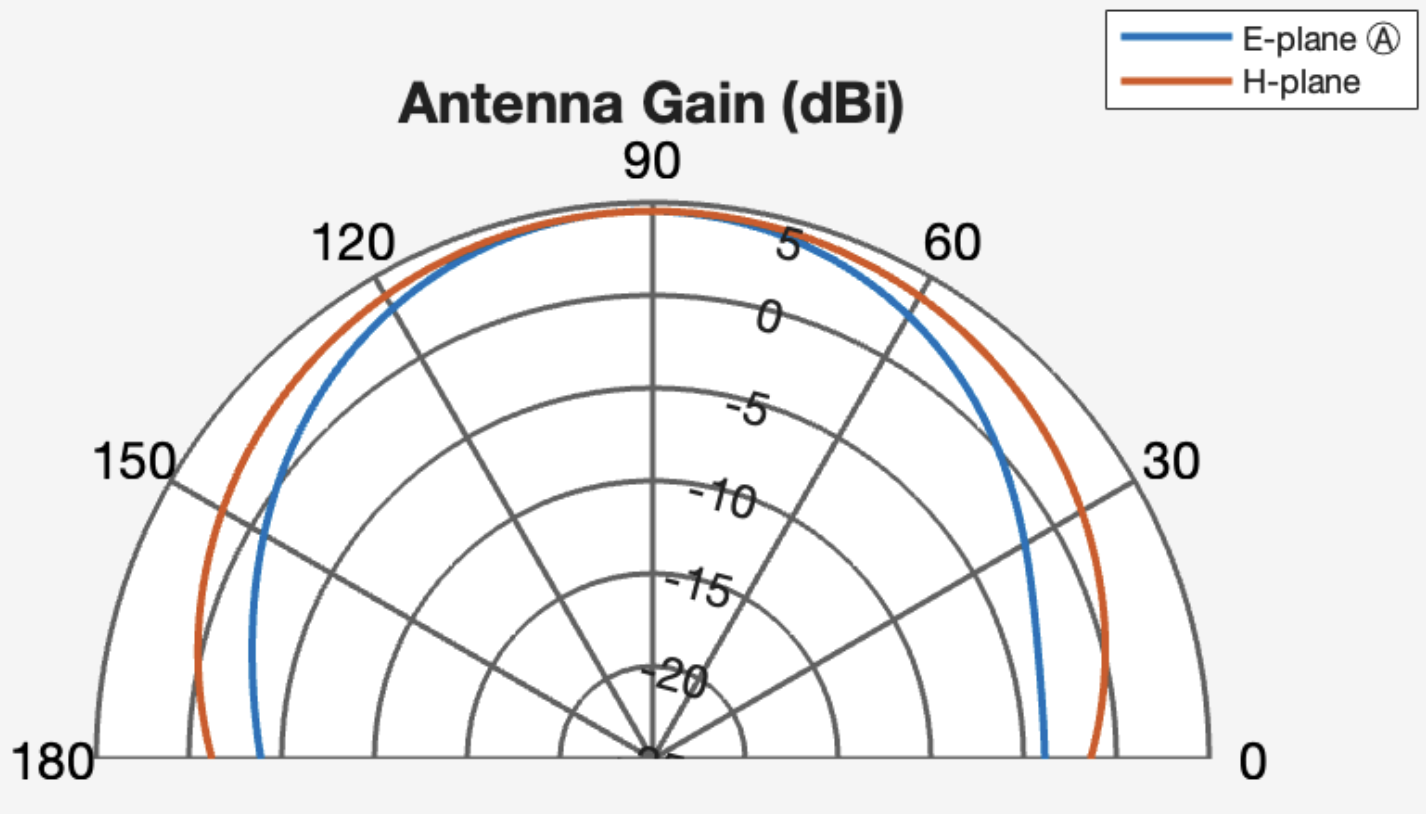
\includegraphics[scale=.3]{figures/antenna_gain_optimization.png}}
        \caption{Antenna gain of the previous version}
        \label{antenna gain of the previous version}
    \end{subfigure}
    \begin{subfigure}{0.45\textwidth}
        \centering
        \adjustbox{height=4cm}{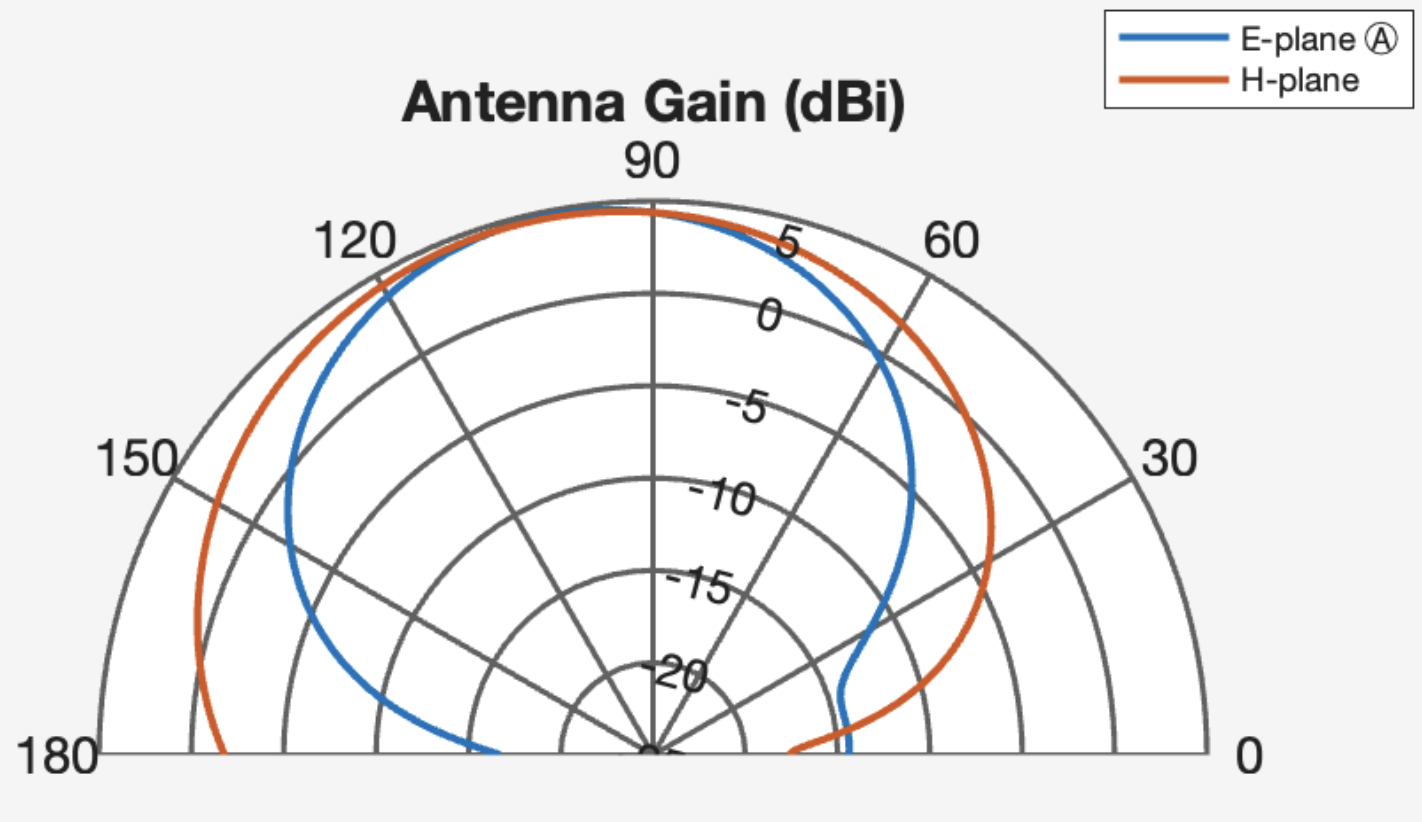
\includegraphics[scale=.3]{figures/antenna_gain_latest.png}}
        \caption{Antenna gain of the final version}
        \label{antenna gain of the final version}
    \end{subfigure}
    \caption{Antenna gain at the elevation angle in EH plane}
    \label{antenna gain at the elevation angle in EH plane}
\end{figure}

Then the antenna could be applied to the simulation. Figure \ref{the view and radiation pattern of the final antenna} illustrates the look and radiation pattern of the final antenna. Algorithm \ref{parameters of the final antenna} demonstrates the final parameters used in the antenna.

\begin{figure}[t]
    \centering
    \begin{subfigure}{0.45\textwidth}
        \centering
        \adjustbox{height=4.8cm}{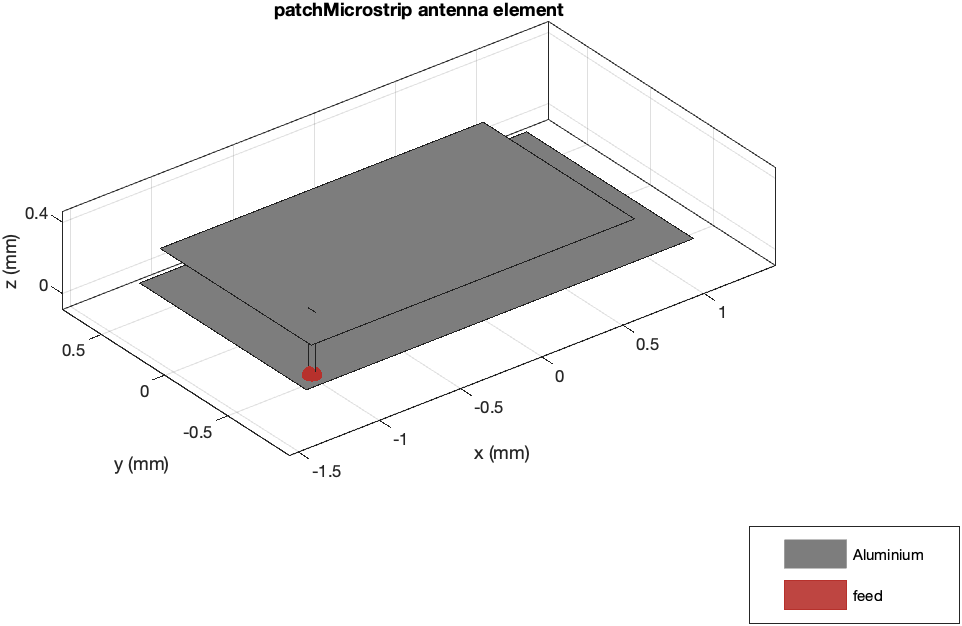
\includegraphics[scale=.3]{figures/antenna_plot_latest.png}}
        \caption{View of the antenna}
    \end{subfigure}
    \begin{subfigure}{0.45\textwidth}
        \centering
        \adjustbox{height=4.8cm}{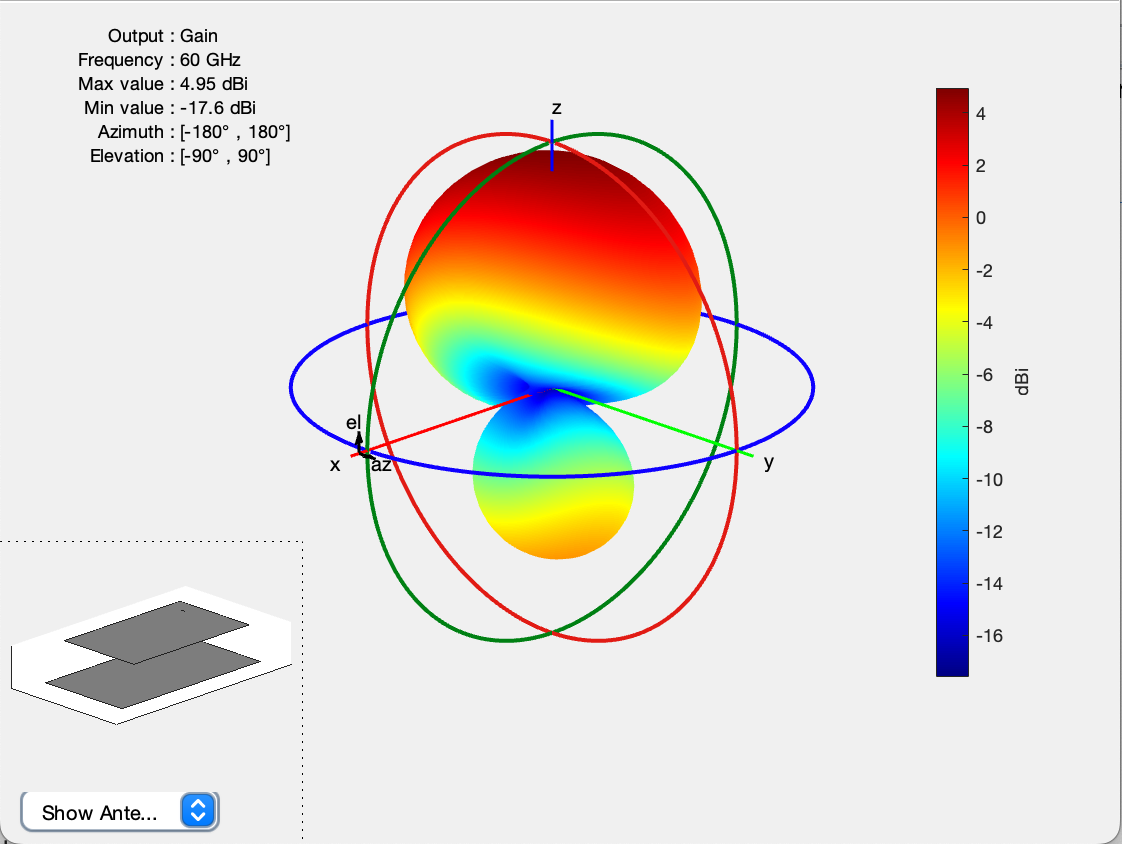
\includegraphics[scale=.3]{figures/radiation_pattern_latest.png}}
        \caption{Radiation pattern of the antenna}
    \end{subfigure}
    \caption{The view and radiation pattern of the final antenna}
    \label{the view and radiation pattern of the final antenna}
\end{figure}

\begin{algorithm}
    \caption{Parameters of the antenna}
    \label{parameters of the final antenna}
    \begin{algorithmic}
        \setstretch{1.2}
        \STATE $antennaObject\ =\ design(patchMicrostrip, 60*1e9);$
        \STATE $antennaObject.Length\ =\ 0.0019908;$
        \STATE $antennaObject.Width\ =\ 0.00093211;$
        \STATE $antennaObject.Height\ =\ 4.8995e-05;$
        \STATE $antennaObject.Substrate.Thickness\ =\ 4.8995e-05;$
        \STATE $antennaObject.GroundPlaneLength\ =\ 0.0023848;$
        \STATE $antennaObject.GroundPlaneWidth\ =\ 0.0010152;$
        \STATE $antennaObject.PatchCenterOffset\ =\ [0.00014792, -6.9634e-08];$
        \STATE $antennaObject.FeedOffset\ =\ [-0.00019916, -0.00014773];$
        \STATE $antennaObject.Conductor.Name\ =\ 'Aluminium';$
        \STATE $antennaObject.Conductor.Conductivity\ =\ 8.8902*1e9;$
        \STATE $antennaObject.Conductor.Thickness\ =\ 0.000762; $
    \end{algorithmic}
\end{algorithm}

\begin{spacing}{1.5}
\textbf{\large{Simulation}}
\end{spacing}

The antenna designed above is exported into the raytracing code. Compared with the simulation process in the previous section, the isotropic antenna needs to be modified into an antenna object at rxsite and txsite settings in ray tracing. The ray tracing view is shown in Figure \ref{view of the ray tracing with beam pattern}. The image on the left shows the effect obtained in the entire scene and the figure on the right illustrates the effect of LOS rays.

\begin{figure}[t]
    \centering
    \begin{subfigure}{0.45\textwidth}
        \centering
        \adjustbox{height=5.2cm}{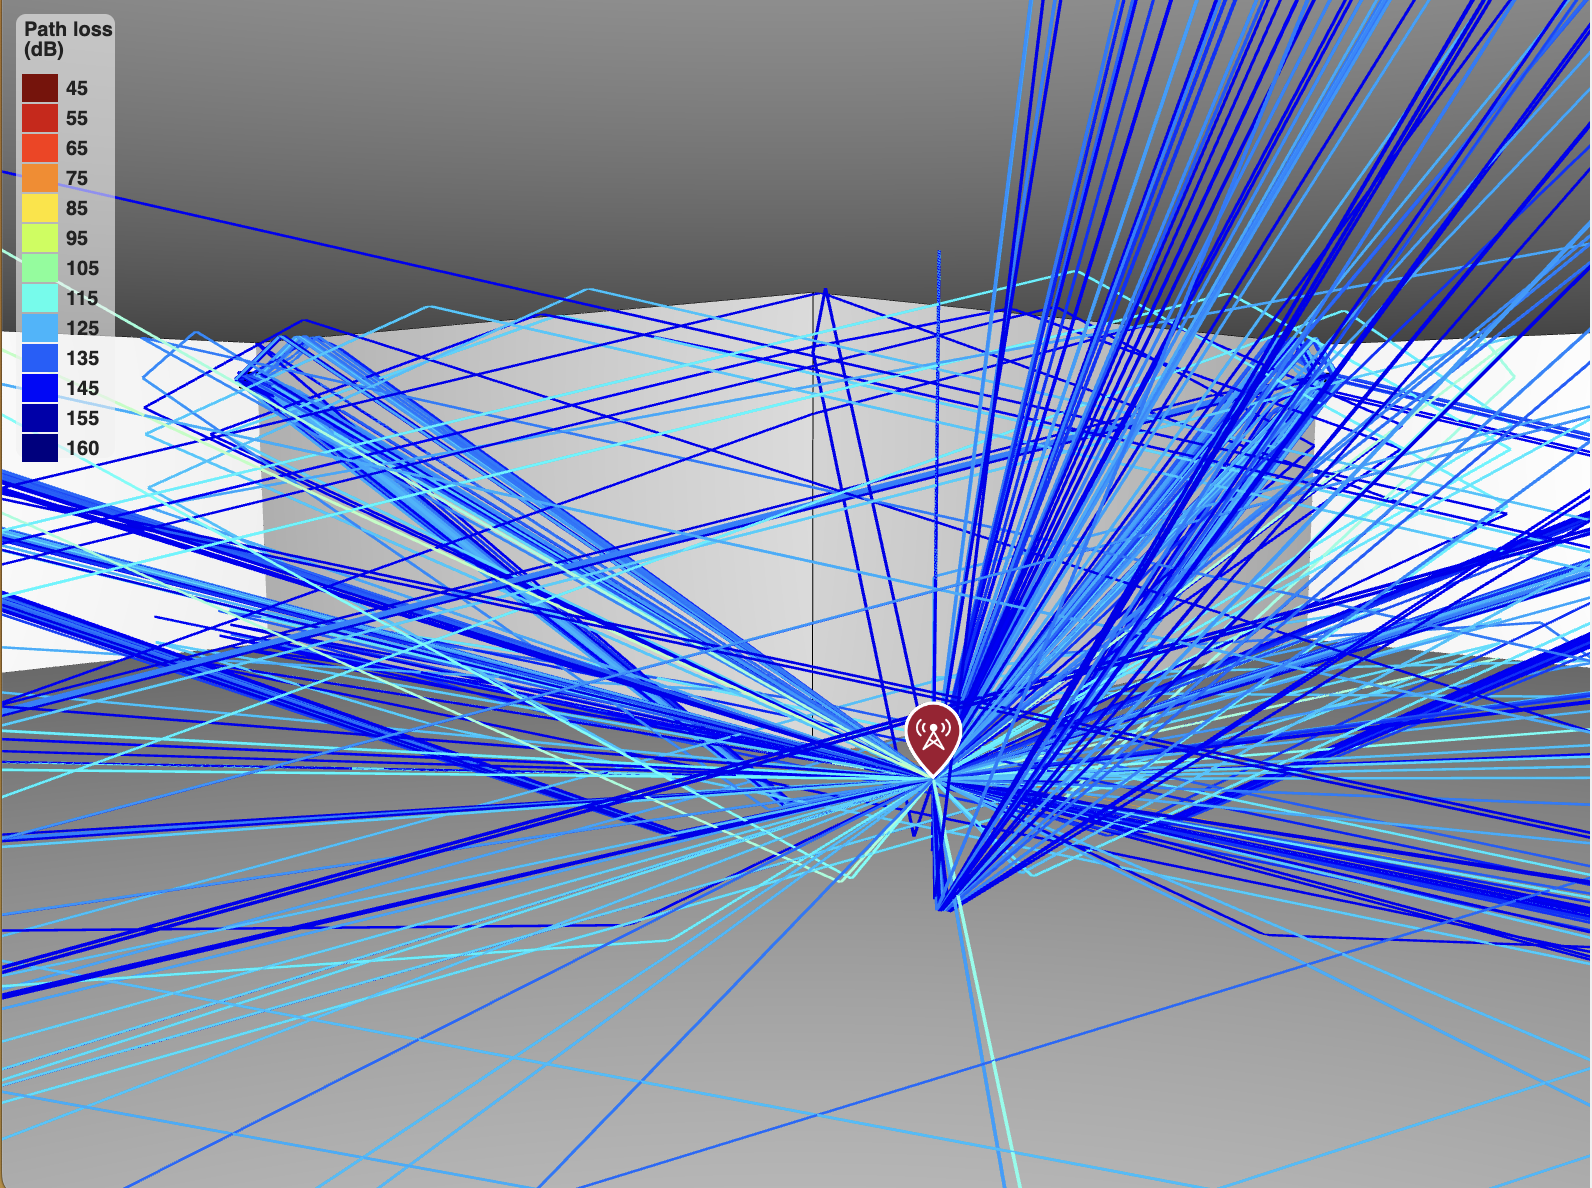
\includegraphics[scale=.3]{figures/beampattern_simulation_left.png}}
    \end{subfigure}
    \begin{subfigure}{0.45\textwidth}
        \centering
        \adjustbox{height=5.2cm}{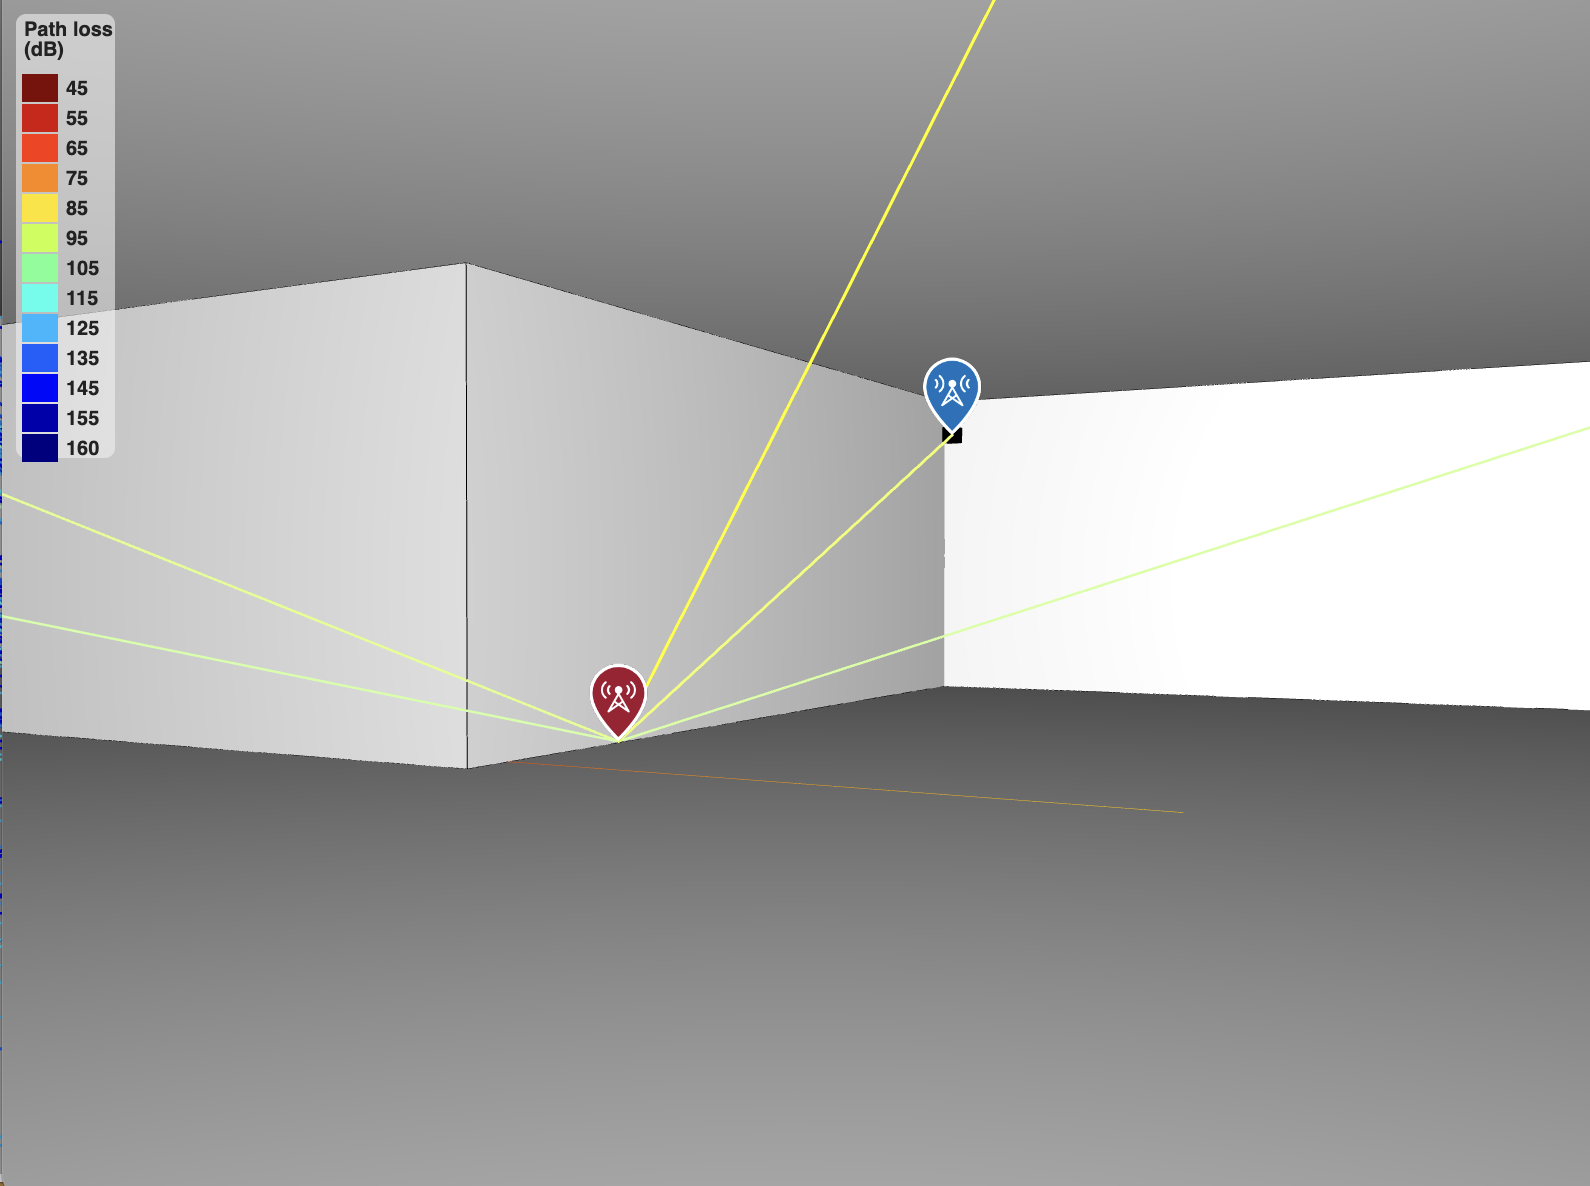
\includegraphics[scale=.3]{figures/beampattern_simulation_right.png}}
    \end{subfigure}
    \caption{View of the ray tracing with beam pattern}
    \label{view of the ray tracing with beam pattern}
\end{figure}

After the addition of the antenna radiation pattern, the changes in the simulation mainly include the following aspects:

\begin{enumerate}[label=\textbullet]
    \item In the previous assumption as formula \ref{gain of the isotropic antenna equation}, the gain of an isotropic antenna is 1, or $0\,\mathrm{dB}$, and the maximum gain of the newly designed antenna is adjusted to $4.4\,\mathrm{dBi}$, which means that at the maximum gain, a better propagation effect can be obtained than with the isotropic antenna. However, according to Figure \ref{antenna gain of the final version}, the gain exceeds $0\,\mathrm{dBi}$ only at a certain angle range in the elevation view, which means that only the rays with AoD in the certain angle range have the stronger power, while at other angles, the gain is not as strong as that of the isotropic antenna. However, most of the rays are out of this angle range.

    \item According to the analysis in the last item, it's known that for most rays, the gain is decreasing. According to formula \ref{path loss formula}, the decrease in gain will lead to an increase in path loss. When the same loss threshold is set in ray tracing, more rays will be over this threshold and be excluded from the cell of rays to be processed later. Table \ref{difference in the amount of rays} shows the difference in the number of rays in three different models, which clearly shows the decrease in the number of rays in the radiation pattern case.

    \begin{table}
    \centering
    \caption{The difference in the number of rays}
    \label{difference in the amount of rays}
    \begin{tabular}{lccccc{1cm}}
        \hline
        \multicolumn{1}{l|}{} & \multicolumn{1}{c|}{Empty room} & \multicolumn{3}{c|}{Room with reflectors} & \multicolumn{1}{c}{Room with furniture}\\
        \hline

        \multicolumn{1}{l|}{Isotropic antenna} & \multicolumn{1}{c|}{202 rays} & \multicolumn{3}{c|}{701 rays} & \multicolumn{1}{c}{1609 rays}\\
        \hline

        \multicolumn{1}{l|}{Radiation pattern antenna} & \multicolumn{1}{c|}{148 rays} & \multicolumn{3}{c|}{588 rays} & \multicolumn{1}{c}{1099 rays}\\
        \hline
    \end{tabular}
    \end{table}

    \item As mentioned in the previous two items, the addition of radiation pattern leads to a decrease in gain and an increase in loss, and this effect is no exception for the rays propagating through the reflector. From Table \ref{difference in the loss of the rays}, it can be seen that the loss increase in the LOS rays and the average as well as median loss value of the overall rays.

    \begin{table}
    \centering
    \caption{The difference in the loss of the rays}
    \label{difference in the loss of the rays}
    \begin{tabular}{lccccccc}
        \hline
        \multicolumn{1}{l|}{} & \multicolumn{1}{c|}{LOS1} & \multicolumn{1}{c|}{LOS2} & \multicolumn{1}{c|}{LOS3} & \multicolumn{1}{c|}{LOS4} & \multicolumn{1}{c|}{LOS5} & \multicolumn{1}{c|}{Average} & \multicolumn{1}{c}{Median}\\
        \hline

        \multicolumn{1}{c|}{Loss with isotropic antenna} & \multicolumn{1}{c|}{98.9} & \multicolumn{1}{c|}{101.3} & \multicolumn{1}{c|}{94.9} & \multicolumn{1}{c|}{99.6} & \multicolumn{1}{c|}{97.8} & \multicolumn{1}{c|}{130.4} & \multicolumn{1}{c}{131.3}\\
        \hline

        \multicolumn{1}{c|}{Loss with radiation pattern} & \multicolumn{1}{c|}{116.0} & \multicolumn{1}{c|}{107.7} & \multicolumn{1}{c|}{108.5} & \multicolumn{1}{c|}{132.2} & \multicolumn{1}{c|}{112.8} & \multicolumn{1}{c|}{131.5} & \multicolumn{1}{c}{132.2}\\
        \hline
    \end{tabular}
    \end{table}

\end{enumerate}

Therefore, in summary, according to the analysis of the above results, with the introduction of the radiation pattern, the overall loss is increasing, but for objects on the ground, the increase is larger, which also makes the signals over the threshold and are excluded from subsequent processing. Therefore, it reduces a lot of interference from surrounding objects and reduces a lot of interference from extremely strong signals caused by surrounding close-range objects compared with isotropic pattern. However, the disadvantage is that, according to Table \ref{difference in the loss of the rays}, the difference between the LOS rays from the reflector and obtained by walls' reflection is not so obvious. 

\section{Reflector radar cross section} \label{Reflector radar cross section}
This section will introduce the generation process of radar cross-section (RCS) and the addition into ray tracing calculation.

\begin{spacing}{1.5}
\textbf{\large{RCS generation}}
\end{spacing}

According to formula \ref{radar cross-section formula}, the max value of RCS depends on the wavelength of the radar system and the edge length of the reflector. But for the anisotropic RCS, it depends on the azimuth and elevation angle of the ray to the reflector as well. The relationship between the RCS value and the angle for the triangular trihedral corner reflector is shown in formula \ref{radar cross-section in dependence of angle formula} \cite{doerry_reflectors_2014}.

\begin{equation}
    \centering
    \sigma_{\text{triangle}}(\psi, \theta) =
    \begin{cases} 
    \frac{4\pi}{\lambda^2}a^4\left(\frac{4c_1c_2}{c_1 + c_2 + c_3}\right)^2 & \text{for } c_1 + c_2 \leq c_3 \\ \\
    \frac{4\pi}{\lambda^2}a^4\left(c_1 + c_2 + c_3 - \frac{2}{c_1 + c_2 + c_3}\right)^2 & \text{for } c_1 + c_2 \geq c_3
    \end{cases},
    \label{radar cross-section in dependence of angle formula}
\end{equation}

where $\psi$ and $\theta$ are the elevation and azimuth angle respectively, $a$ is the length of the reflector's edge, and $c_1, c_2, c_3$ represent the coordinates in euclidean coordinate system which are each assigned as

\begin{equation}
    \left.
    \begin{array}{l}
    c_1 \\
    c_2 \\
    c_3
    \end{array}
    \right\}
    =
    \left\{
    \begin{array}{l}
    \sin \psi \\
    \cos \psi \sin \theta \\
    \cos \psi \cos \theta
    \end{array}
    \right.
\end{equation}

such that $c_1 \leq c_2 \leq c_3$. The peak of the RCS occurs in the direction that forms an angle $tan^{-1}(1/\sqrt{2})$ or approximately 35.26 degrees with any side of the triangular corner reflector, which is also called the bore-sight line. It should be pointed out that for reflectors of different shapes, the formula of the max RCS value and the value related to angles are different. The following RCS value with angle is plotted based on formula \ref{radar cross-section in dependence of angle formula}, where Figure \ref{rcs related to azimuth and elevation angles} represents the RCS value at different azimuth and elevation angle, and Figure \ref{rcs related to azimuth as el=35deg} represents the variation of RCS with azimuth angle when elevation angle is along the bore-sight line, i.e. 35 degrees, where the peak happens at the 35 degrees azimuth angle.

\begin{figure}
    \centering
    \begin{subfigure}{0.45\textwidth}
        \centering
        \adjustbox{height=5.2cm}{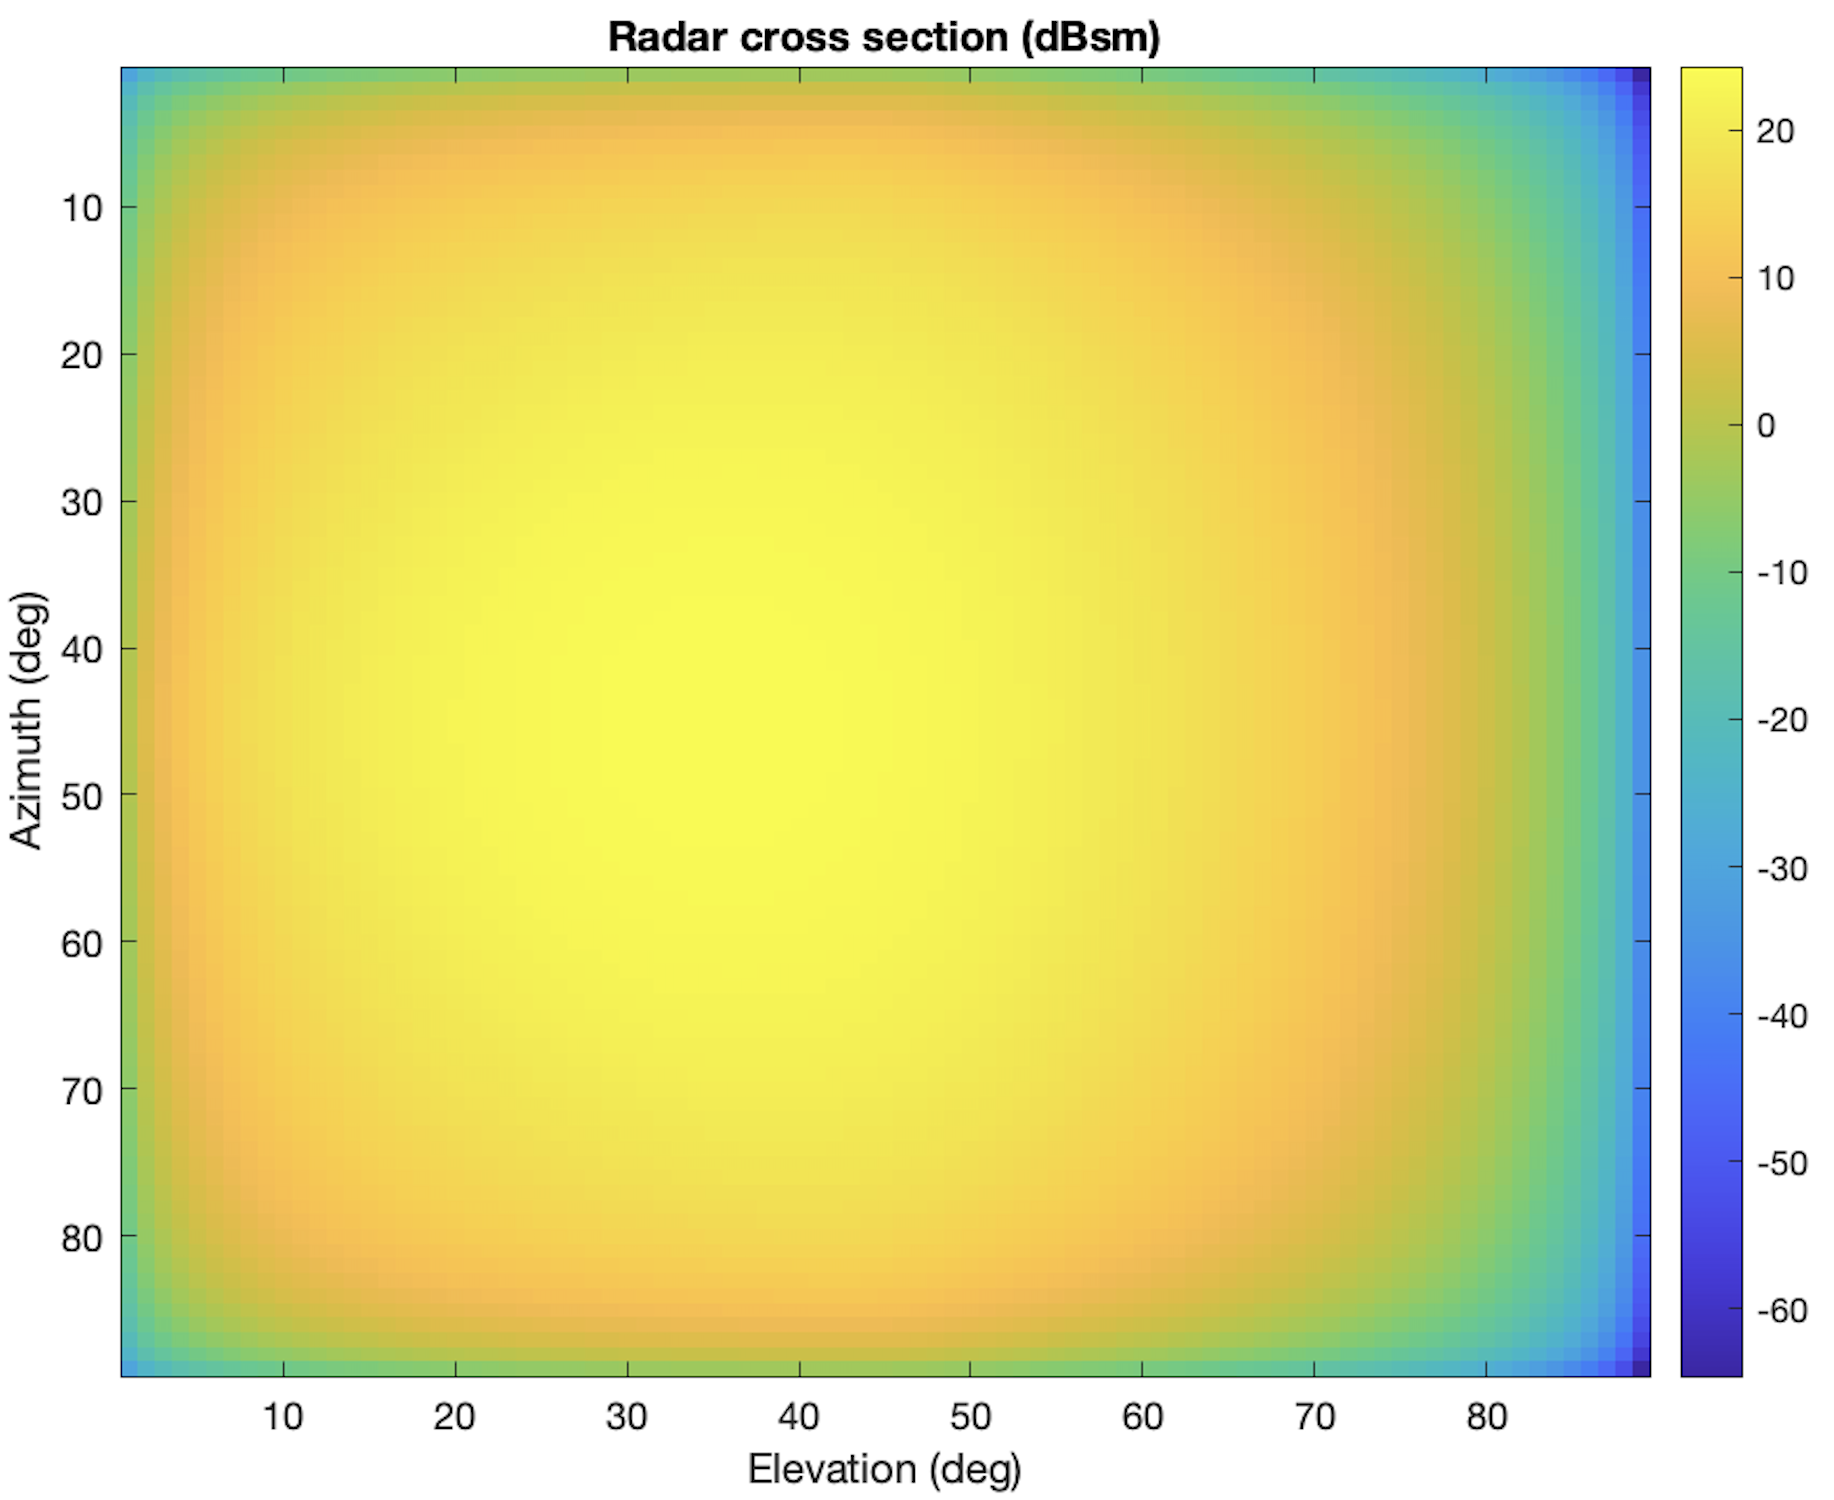
\includegraphics[scale=.4]{figures/rcs_pattern_dbsm.png}}
        \caption{RCS related to az and el angles}
        \label{rcs related to azimuth and elevation angles}
    \end{subfigure}
    \begin{subfigure}{0.45\textwidth}
        \centering
        \adjustbox{height=5.2cm}{\includegraphics[scale=.2]{figures/rcs_pattern_dbsm_35ele.png}}
        \caption{RCS related to azimuth as $el=35^{\circ}$}
        \label{rcs related to azimuth as el=35deg}
    \end{subfigure}
    \caption{View of the RCS value related to the angles}
    \label{view of rcs value related to the angles}
\end{figure}

To obtain the anisotropic pattern of RCS, the RCS formula in MATLAB can be used for simulation. The input parameters include the simulated object, frequency, and the range of azimuth and elevation information. Before applying it to all az and el ranges, first use the tetrahedral object provided by MATLAB \cite{rcs_plausibility} for plausibility check, which can be used as a baseline to check whether this method can be effectively applied to the triangular corner reflector with the parameters in our radar system. First, use its default $700\,\mathrm{MHz}$ frequence and get the 2D RCS plot as the elevation angle is 0 degrees shown in Figure \ref{view of the rcs for tetrahedral object with default parameters}.

\begin{figure}[t]
    \centering
    \begin{subfigure}{0.45\textwidth}
        \centering
        \adjustbox{height=6cm}{\includegraphics[scale=.3]{figures/mesh_tetrahedral.png}}
    \end{subfigure}
    \begin{subfigure}{0.45\textwidth}
        \centering
        \adjustbox{height=6cm}{\includegraphics[scale=.3]{figures/rcs_tetrahedral.png}}
    \end{subfigure}
    \caption{View of the RCS for the tetrahedral object with default parameters}
    \label{view of the rcs for tetrahedral object with default parameters}
\end{figure}

Since the frequency in our radar system is determined as $60\,\mathrm{GHz}$ and the edge length of the reflector is roughly $20\,\mathrm{cm}$, the tetrahedral object provided by Matlab can still be used to test the influence of the change of frequency, as well as size on the plot of the RCS. To speed up the simulation effect, the method of moments (MoM) solver will be used in this case. Figure \ref{view of the rcs for tetrahedral object with scaled parameters} illustrates the mesh of the tetrahedral object and its RCS plot with the scaled parameters. From the results, it can be seen that it mainly affects the peak value of RCS but has little effect on the overall shape. Therefore, the effect of scaling parameters on RCS is reasonable.

\begin{figure}[t]
    \centering
    \begin{subfigure}{0.45\textwidth}
        \centering
        \adjustbox{height=6cm}{\includegraphics[scale=.3]{figures/mesh_tetrahedral_scaled.png}}
    \end{subfigure}
    \begin{subfigure}{0.45\textwidth}
        \centering
        \adjustbox{height=6cm}{\includegraphics[scale=.3]{figures/rcs_tetrahedral_scaled.png}}
    \end{subfigure}
    \caption{View of the RCS for the tetrahedral object with scaled parameters}
    \label{view of the rcs for tetrahedral object with scaled parameters}
\end{figure}

The next step is to completely replace the simulated object and frequency information with those in our radar system with using the MoM solver. Figure \ref{view of the rcs for triangular corner reflector} demonstrates the result of the triangular corner reflector at the 0 degree elevation angle. It shows that the angle of 40 degrees from 0 degrees to either side will reach the perpendicular angle of the triangular corner reflector's two sides roughly, that is, the peak value of RCS, which satisfies the expectation of the triangular corner reflectors's RCS as above. But the maximum value still occurs when both azimuth and elevation are 0 degree, because the plot is shifted it to 0 degree. This means that the RCS function is still valid for the type, size of the reflector, and frequency settings in our radar system, so we can loop in the angle range of azimuth and elevation following to get the 3D RCS pattern.

\begin{figure}[t]
    \centering
    \begin{subfigure}{0.45\textwidth}
        \centering
        \adjustbox{height=6cm}{\includegraphics[scale=.3]{figures/mesh_cr.png}}
    \end{subfigure}
    \begin{subfigure}{0.45\textwidth}
        \centering
        \adjustbox{height=6cm}{\includegraphics[scale=.3]{figures/rcs_cr.png}}
    \end{subfigure}
    \caption{View of the RCS for triangular corner reflector}
    \label{view of the rcs for triangular corner reflector}
\end{figure}

\begin{algorithm}
    \caption{Pseudo code of the RCS generation}
    \label{pseudo code of the rcs generation}
    \renewcommand{\algorithmicrequire}{\textbf{Input:}}
    \renewcommand{\algorithmicensure}{\textbf{Output:}}
    
    \begin{algorithmic}[1]
        \REQUIRE $reflector\_model.stl$
        \ENSURE $RCS$

        \STATE $p\ =\ platform;$
        \STATE $p.FileName\ =\ 'reflector\_model.stl';$
        \STATE $p.Units\ =\ 'm';$
        
        \STATE $mesh(p,\ MaxEdgeLength=0.002)$
        
        \STATE $rcs\_pattern\_dbsm\ =\ zeros(360, 360);$
        \FOR{az=1:2:360}
            \FOR{ele=1:2:360}
                \STATE $rcs\_dbsm\ =\ rcs(p,\ 60e9,\ az,\ ele,\ Solver='MOM',\ EnableGPU=0);$
                \STATE $rcs\_pattern\_dbsm(az, ele)\ =\ rcs\_dbsm;$
            \ENDFOR
        \ENDFOR
        
    \end{algorithmic}   
\end{algorithm}

Since every angle within the angle range must be simulated, the computational complexity of this task is very dependent on the hardware. Therefore, to speed it up, the mesh size can be appropriately reduced and a proportionally scaled reflector model can be used. After the simulation, the above formula can be used to perform an overall proportional calculation to quickly obtain the RCS value. Algorithm \ref{pseudo code of the rcs generation} shows the method for calculating the 3D RCS pattern, which is applied to both triangular corner reflector and octahedral reflector.

In this way, the anisotropic 3D RCS pattern can be simulated. Figure \ref{3d rcs view for the triangular corner reflector} shows the 3D RCS plot of the triangular corner reflector, and Figure \ref{3d rcs view for the octahedral reflector} shows the 3D RCS plot of the octahedral reflector.

\begin{figure}[t]
    \centering
    \begin{subfigure}{0.45\textwidth}
        \centering
        \adjustbox{height=6cm}{\includegraphics[scale=.3]{figures/trihe_3d_rcs.png}}
        \caption{3D RCS view for the triangular reflector}
        \label{3d rcs view for the triangular corner reflector}
    \end{subfigure}
    \begin{subfigure}{0.45\textwidth}
        \centering
        \adjustbox{height=6cm}{\includegraphics[scale=.3]{figures/octa_3d_rcs.png}}
        \caption{3D RCS view for the octahedral reflector}
        \label{3d rcs view for the octahedral reflector}
    \end{subfigure}
    \caption{View of the 3D RCS for reflectors}
    \label{view of the rcs for reflectors}
\end{figure}

\begin{spacing}{1.5}
\textbf{\large{Ray tracing}}
\end{spacing}

Substitute the anisotropic RCS values related to azimuth and elevation angle into the ray tracing. Since RCS only affects the loss of rays passing through the reflectors, which corresponds to the LOS rays in our radar system, the original isotropic max RCS value is replaced. However, to reduce the computational complexity during the simulation, the angle resolution as written in Algorithm \ref{pseudo code of the rcs generation} is two degrees, but the accuracy in the decimal places of this AoD is much higher so that the resolution of two degrees cannot meet its requirements. Therefore, here we use the two-dimensional linear interpolation method to obtain the corresponding RCS value.

In most cases, the incident angle of rays is difficult to accurately reach the bare sight line or perpendicular to the reflector, which means that the RCS obtained is likely to be much smaller than the isotropic RCS value used in the previous sections, which will lead to an increase in the loss of LOS rays and the loss advantage of LOS will be further reduced compared to the previous loss. Table \ref{difference of the LOS rays' loss between isotropic RCS and realistic RCS} shows the difference in LOS rays' loss between the isotropic and anisotropic RCS value under the condition of the antenna's radiation pattern.

\begin{table}
    \centering
    \caption{The difference of the LOS rays' loss between isotropic and anisotropic RCS}
    \label{difference of the LOS rays' loss between isotropic RCS and realistic RCS}
    \begin{tabular}{lccccc}
        \hline
        \multicolumn{1}{l|}{} & \multicolumn{1}{c|}{LOS1} & \multicolumn{1}{c|}{LOS2} & \multicolumn{1}{c|}{LOS3} & \multicolumn{1}{c|}{LOS4} & \multicolumn{1}{c}{LOS5}\\
        \hline

        \multicolumn{1}{l|}{Loss with isotropic RCS} & \multicolumn{1}{c|}{116.0} & \multicolumn{1}{c|}{107.7} & \multicolumn{1}{c|}{108.5} & \multicolumn{1}{c|}{132.2} & \multicolumn{1}{c}{112.8}\\
        \hline

        \multicolumn{1}{l|}{Loss with realistic RCS} & \multicolumn{1}{c|}{143.4} & \multicolumn{1}{c|}{129.9} & \multicolumn{1}{c|}{132.6} & \multicolumn{1}{c|}{161.9} & \multicolumn{1}{c}{139.4}\\
        \hline
    \end{tabular}
\end{table}

One solution to this problem is to increase the size of the reflector. According to formula \ref{radar cross-section formula}, its max value is affected by the edge length and wavelength. For a radar system, the wavelength is constant, so only the edge length can be changed. If the size of a reflector is doubled, that is, $a$ becomes $2a$, then for a triangular corner reflector, its RCS max value will become 16 times in the linear scale, which is equivalent to an increase of 12dB, that is, the overall loss is reduced by 12dB, which is helpful to alleviate the increase in loss caused by the anisotropic RCS pattern.

The octahedral reflector can be understood as a combination of eight triangular corner reflectors, so the RCS value in each corner is equivalent to that of the triangular reflector, so the method above can be applied to the octahedral reflector in the same way. For the octahedral reflector, it is usually not necessary to place it in the corner but can be directly hung on the ceiling of the room, so it is mainly the four triangular reflectors at the bottom that play the role.

In addition, to make the entire code structure more unified, when using isotropic RCS, a matrix of the same size as the anisotropic RCS will be generated, and its value will use the maximum value in any direction.

\section{Motion of robot} \label{Motion of robot}
In this section, we will design a motion trajectory for the robot randomly and smoothly. In this motion trajectory, we can obtain the position and velocity at any time, and the effect changes in ray tracing and subsequent signal processing. Meanwhile, we will also get an orientation parameter, which affects the direction of the robot and thus the orientation of the antenna's radiation pattern.

\begin{spacing}{1.5}
\textbf{\large{Trajectory generation}}
\end{spacing}
For the generation of motion trajectory, the $waypointTrajectory$ function provided in Matlab \cite{trajectory_generation} will be used. The principle is that given several positions and the time points of reaching the corresponding positions, this function will generate a motion path that passes through specific positions at a specified time. Therefore, as the AMR moves between each position, the offset of the position as well as a series of positions, directions, and velocities at any sampling time will be generated.

Some important input parameters in this function include:
\begin{enumerate}[label=\textbullet]
    \item $Waypoints$ is specified as an N-by-3 matrix which represents N positions in the three-dimensional scene. In our scenario, the robot moves along a trajectory. Considering that there are different objects such as furniture in different room models, we will take the model of the furniture into account and generate a closed-loop trajectory surrounding the wall or furniture, in which ten positions are specified.

    \item $TimeOfArrival$ indicates the time that it takes to reach each specified point, so the number should correspond to the number of points. If ten points were specified in the previous item, ten time points will also be set here.

    \item $SampleRate$ represents the time interval for collecting parameters during the motion process. The default is $100\,\mathrm{Hz}$ and will be maintained here.

    \item The input parameters can also add information such as velocity, acceleration, or orientation when passing through a specified point. To make the generated trajectory more random, this information will not be specified.

    \item Since the velocity or acceleration of the AMR at a given moment obtained by the function is a relative quantity to the ground, the ground speed will affect these values. As the robot in our radar system moves in the room, that is, the room and the ground remain stationary, the ground speed is determined here by default as $0\,\mathrm{m/s}$.
\end{enumerate}

The output of the function includes five parameters, namely position, orientation, velocity, acceleration, and angular velocity. Since the radar system focuses on the range and Doppler effect between the robot and the target point, only the position, orientation, and velocity will be needed here. The dimensions of the three parameters are $N\times 3$, $N\times 4$ and $N\times 3$ respectively. Position and velocity are three-dimensional coordinates, while orientation uses quaternion, which will be introduced in the next part. The obtained $N$ dimension is affected by both sampling rate and running time, and the calculation formula is

\begin{equation}
    \centering
    N = trajectory.SampleRate \times (time\_points(end) - time\_points(1)).
\end{equation}

After getting the position, the motion trajectory could be drawn. Figure \ref{view of the motion trajectory} shows the motion trajectory of the robot in the room, where the specified positions in the trajectory are marked with a solid red dot, and each sampling point is marked with a short line.

\begin{figure}
	\centering
	\includegraphics[scale=.3]{figures/trajectory.png}
	\caption{View of the motion trajectory}
	\label{view of the motion trajectory}
\end{figure}

The following method will be used to obtain the position, velocity, and corresponding orientation at each moment required for the simulation of the radar system. Specify a time point within the first and last time point of the generated path, and use the total duration and sampling frequency information to find the corresponding upper and lower sampled time points and their corresponding position, velocity, and orientation data. One-dimensional linear interpolation is performed along each dimension of the three data and recombined to solve the problem of different dimensions of different data. Meanwhile, the use of linear interpolation can effectively reduce the required sampling frequency and reduce the computational complexity of the entire system, which is a compromise.

\begin{spacing}{1.5}
\textbf{\large{Orientation of the robot}}
\end{spacing}

As mentioned in the previous part, the orientation obtained by the $waypointTrajectory$ function is a quaternion, which will be used to define the rotation of the robot and the antenna's radiation pattern. If a quaternion is written as $q(w, x, y, z)$, the conversion \cite{quaternion_transform} between it and the rotation matrix is

\begin{equation}
    \centering
    q(w, x, y, z) ==> \begin{bmatrix}
    1 - 2y^2 - 2z^2 & 2xy + 2wz & 2xz - 2wy \\
    2xy - 2wz & 1 - 2x^2 - 2z^2 & 2yz + 2wx \\
    2xz + 2wy & 2yz - 2wx & 1 - 2x^2 - 2y^2
    \end{bmatrix}.
\end{equation}

In our radar system, the specific solution is to use the $quat2eul$ function to convert quaternions into Euler angles, and then convert Euler angles into angles of rotation around an axis with the $rad2deg$ function. Since the antenna is always located on the robot platform, the axis of rotation defaults to the z-axis of the robot, and the obtained rotation angle can be applied to the antenna's radiation pattern.

There are two configurable parameters in the antenna object, called $Tilt$ and $TiltAxis$, where $Tilt$ is set to the rotation angle and $TiltAxis$ to its z-axis direction. Figure \ref{view of the default and orientated radiation pattern} shows the difference in the shape of the antenna radiation pattern with elevation angle before and after the orientation when azimuth is 0 defree.

\begin{figure}[t]
    \centering
    \begin{subfigure}{0.45\textwidth}
        \centering
        \adjustbox{height=6cm}{\includegraphics[scale=.3]{figures/original_pattern.png}}
    \end{subfigure}
    \begin{subfigure}{0.45\textwidth}
        \centering
        \adjustbox{height=6cm}{\includegraphics[scale=.3]{figures/orientated_pattern.png}}
    \end{subfigure}
    \caption{View of the default and rotated radiation pattern}
    \label{view of the default and orientated radiation pattern}
\end{figure}

Figure \ref{view of the default and orientated ray tracing} shows the comparison of ray tracing effects before and after the introduction of the orientation information for the same given position and velocity. It can be observed that with the introduction of orientation, the loss of rays changes, because the radiation pattern of the antenna is not completely symmetrical around the z-axis, so the rotation will cause the change of the gain value in different directions, which in turn affects the loss value.

\begin{figure}[!htb]
    \centering
    \begin{subfigure}{0.45\textwidth}
        \centering
        \adjustbox{height=5cm}{\includegraphics[scale=.3]{figures/original_ray_tracing.png}}
    \end{subfigure}
    \begin{subfigure}{0.45\textwidth}
        \centering
        \adjustbox{height=5cm}{\includegraphics[scale=.3]{figures/orientated_ray_tracing.png}}
    \end{subfigure}
    \caption{View of the original and rotated ray tracing}
    \label{view of the default and orientated ray tracing}
\end{figure}

\chapter{Radar signal processing} \label{Radar signal processing}
This chapter will use the signals obtained in the previous chapters and the processed baseband signal to compute range-Doppler maps and do the CFAR detection, to observe the target points in the map and verify the accuracy of the toolchain.

\section{Range-Doppler map} \label{Range-Doppler map}

To convert the discretized baseband signal into the range-Doppler map, a two-dimensional FFT operation \cite{kronauge_new_2014} is required to convert the time domain signal into the frequency domain and analyze the frequency domain components of the signal, thereby analyzing the range and velocity related to the targets in the spectrum. In our case, the FFT equation is as follows:

\begin{equation}
F(u,v) = \sum_{x=0}^{N_s-1} \sum_{y=0}^{N_p-1} f(x,y) e^{-j 2 \pi \left( \frac{ux}{N_s} + \frac{vy}{N_p} \right)},
\end{equation}
where $N_s=256$, $N_p=32$. The 2D FFT can also be viewed as two 1D FFTs, where one 1D FFT is used to extract Doppler effect information along the slow time axis, and the other 1D FFT is used to extract range information along the fast time axis. 

Due to the direction of the velocity, the Doppler frequencies are zero-centered after FFT, and approaching and moving away from the target point means the positive speed and negative speed respectively.

Since the size of the discretized baseband signal is $(32, 256)$, the result after FFT remains the same size. According to the velocity and range resolution analyzed above, set the resolution of the x- and y-axis coordinates as well as the range of velocity and range in the range-Doppler map, and take the absolute value after FFT to draw. According to the conclusions in Table \ref{parameters of the radar system}, the resolutions of velocity and range will be $0.355\,\mathrm{m/s}$ and $7.5\,\mathrm{cm}$ respectively, and the range between target points and the robot will be in the range of $[0, 20\,\mathrm{m})$, and the range of velocity will be $[-5.68\,\mathrm{m/s}, 5.33\,\mathrm{m/s}]$.

Meanwhile, since the amplitude is defined as voltage in the radar model, and the subsequent CFAR detection needs to be analyzed based on power, the power value is obtained based on the overall resistance of the radar system and the voltage value. Here, various graphs will be drawn based on different units, including voltage V, power in watt, and in units such as dBW and dBm.

The following part will present various comparisons of the range-Doppler map obtained according to different classifications of cases, while the evaluation and analysis will be carried out in section \ref{Evaluation} in conjunction with CFAR detection.

\section{CFAR detection} \label{CFAR detection}

Another signal processing method is called constant false alarm rate (CFAR) detection, which is a common target detection method used to detect target signals in background noise and ensure that the false detection probability remains constant. A threshold is usually set for the target detection. When the signal amplitude is larger than this threshold, it means that the target object exists, otherwise it does not exist.

\begin{equation}
    RD(n_s, n_p) \underset{H_0}{\overset{H_1}{\gtrless}} \lambda,
\end{equation}
where $RD(n_s, n_p)$ represents the amplitude of the range-Doppler map along the both fast and slow time axis and $\lambda$ means the corresponding threshold. If ensure that the false alarm rate is constant, the threshold should satisfy the following formula:

\begin{equation}
P_{FA} = \int_{\lambda}^{\infty} f_X(x \mid H_0) \, dx,
\end{equation}
where $H_0$ denotes the hypothesis that there is no target object at the detection position, while $H_1$ indicates that there is a target at the detection location. $f_X(x\mid H_0)$ denotes the probability density function (PDF) of the signal without targets. $P_{FA}$ represents the probability of false alarm.

The above calculation method is based on the assumption that the PDF of noise and signal is known, but in fact, noise and signal are non-homogeneous and have no known distribution. Therefore, in this case, the method is to establish a detection window with the detection position as the center, calculate the average and variance of the signal power at the surrounding position, and substitute the target false alarm rate and threshold factor into the power information to obtain a threshold \cite{cfar}. The center detection position is called the cell under test (CUT) and there are guard cells and reference cells surrounding it. If the threshold is exceeded, it is considered that the object exists, otherwise it does not exist. The average noise power at surrounding locations \cite{cfar_calculation} should be as

\begin{equation}
P_n = \frac{1}{N_r} \sum_{i=1}^{N_r} RD(n_s, n_p),
\end{equation}

where $N_r$ is the total number of reference cells. Assuming there is only one target in each detection position, the threshold factor \cite{cfar_calculation} is calculated as

\begin{equation}
\alpha = N_r \left( P_{\text{FA}}^{-1/N_r} - 1 \right).
\end{equation}

The number of guard cells and reference cells is selected empirically. Here, the guard cells are expanded by one layer in the range and velocity directions. The reference cells are expanded by 10 columns in the range direction and 5 rows in the velocity direction, respectively. That is, there are 8 guard cells and 290 reference cells. Therefore, along the edge of the range-Doppler map, there will be some positions that cannot be used to detect the presence of objects. The yellow part in Figure \ref{cfar_range} can be used as CUT, while the blue part can only be used as the reference cells.

\begin{figure}[t]
	\centering
	\includegraphics[scale=.2]{figures/cfar_range.png}
	\caption{The detectable range on CFAR}
	\label{cfar_range}
\end{figure}

According to the calculation of range resolution in the previous section, each cell along x-axis represents the range of $7.5\,\mathrm{cm}$, and 11 layers of cells mean $82.5\,\mathrm{cm}$, which is much smaller than the minimum range of $3.5\,\mathrm{m}$, so it can be ignored. Similarly, for velocity resolution, each grid represents the speed of $0.355\,\mathrm{m/s}$, and 6 grids mean a speed of $2.13\,\mathrm{m/s}$. Since the maximum speed that the robot can move is $2\,\mathrm{m/s}$ and the maximal velocity of the RD map is above $5\,\mathrm{m/s}$, the velocity condition is met as well.

According to the above analysis, the $CFARDetector2D$ function in Matlab can be used to detect the position that meets the specified false alarm rate. For the color in the CFAR map, the RD value at the CUT position is divided by the maximum filtered RD value among all the target positions, and the normalization operation is performed to indicate the magnitude of its amplitude, which can also indicate the probability of the target object appearing here. The results of the CFAR detection are as follows. The order is similar as the RD map, but the first different unit is removed and replaced with different parameters in CFAR. Additionally, the red crosses mean the corresponding relative range and velocity to the radar for each LOS reflector.


\section{Result and evaluation} \label{Evaluation}

This section will show the result of both range-Doppler map and CFAR plot in nine aspects, namely range-Doppler map in different units, in the types of the models, with the anisotropic radiation pattern, with the anisotropic RCS pattern, with various numbers and arrangement of reflectors, with the motion of the robot, in different transmitter power, with some other values of the parameters in the raytracing, and the influence of the CFAR's parameters. Meanwhile, the results will be evaluated and verify the reasonability of these changes and the correctness of the radar system on detecting the range and velocity of the targets.

According to the above part, the range-Doppler map can be saved in four units, including V, W, dBW, and dBm. In the empty room model, according to the default position [3, -2, 0.5] and velocity [1, 2, 0], Figure \ref{range doppler map in different units} demonstrates the effect in different units respectively. Although the principle of the CFAR detector is based on the square unit, in our case, is the watt. But we can still apply CFAR detector on the range-Doppler matrix in watt, but plot in dBm after estimating the CFAR targets. Figure \ref{cfar plot in different units} shows the CFAR plots in various units as the same order as range-Doppler maps.

For RD maps drawn using different units, a matrix with W as the unit is usually used to calculate CFAR detection, but for relatively far targets such as targets close to $20\,\mathrm{m}$, using the unit dBm can effectively reduce the difference of the amplitude at all positions, i.e. after applying the CFAR mask the normalization can be based on the logarithm value although CFAR mask only process the power input. When the SNR value is high enough, the peak of the far targets can be more clearly seen in the dBm graph.

\begin{figure}[t]
    \centering
    \begin{subfigure}{0.45\textwidth}
        \centering
        \adjustbox{height=6cm}{\includegraphics[scale=.3]{figures/1r_empty_V.png}}
        \caption{RD map in unit voltage (V)}
        \label{1r_empty_V}
    \end{subfigure}\hspace{0.5cm}
    \begin{subfigure}{0.45\textwidth}
        \centering
        \adjustbox{height=6cm}{\includegraphics[scale=.3]{figures/1r_empty_W.png}}
        \caption{RD map in unit power (W)}
        \label{1r_empty_W}
    \end{subfigure}
    \begin{subfigure}{0.45\textwidth}
        \centering
        \adjustbox{height=6cm}{\includegraphics[scale=.3]{figures/1r_empty_dBW.png}}
        \caption{RD map in unit dBW}
        \label{1r_empty_dBW}
    \end{subfigure}\hspace{0.5cm}
    \begin{subfigure}{0.45\textwidth}
        \centering
        \adjustbox{height=6cm}{\includegraphics[scale=.3]{figures/1r_empty_dBm.png}}
        \caption{RD map in unit dBm}
        \label{1r_empty_dBm}
    \end{subfigure}
    \caption{Range-Doppler map in different units}
    \label{range doppler map in different units}
\end{figure}

\begin{figure}[t]
    \centering
    \begin{subfigure}{0.45\textwidth}
        \centering
        \adjustbox{height=6cm}{\includegraphics[scale=.3]{figures/1c_empty_V.png}}
        \caption{CFAR plot in unit voltage (V)}
        \label{1c_empty_V}
    \end{subfigure}\hspace{0.5cm}
    \begin{subfigure}{0.45\textwidth}
        \centering
        \adjustbox{height=6cm}{\includegraphics[scale=.3]{figures/1c_empty.png}}
        \caption{CFAR plot in unit power (W)}
        \label{1c_empty}
    \end{subfigure}
    \begin{subfigure}{0.45\textwidth}
        \centering
        \adjustbox{height=6cm}{\includegraphics[scale=.3]{figures/1c_empty_dBW.png}}
        \caption{CFAR plot in unit dBW}
        \label{1c_empty_dBW}
    \end{subfigure}\hspace{0.5cm}
    \begin{subfigure}{0.45\textwidth}
        \centering
        \adjustbox{height=6cm}{\includegraphics[scale=.3]{figures/1c_empty_dBm.png}}
        \caption{CFAR plot in unit dBm}
        \label{1c_empty_dBm}
    \end{subfigure}
    \caption{CFAR plot in different units}
    \label{cfar plot in different units}
\end{figure}

Since in CFAR detection, the range-Doppler matrix in W is processed, all the comparisons below will only show the maps in power (W). This item compares the maps obtained in the empty room model, with reflectors, with the furniture, and plausibility model. Figure \ref{range doppler map in different models} demonstrates the maps in four different room models. Figure \ref{cfar detection in different models} shows the CFAR detection in different models. To ensure that the number of reflectors for each model is the same, the position of the robot is set as (3, 2, 1).

For the item using different models, taking the empty room model as the baseline, for the case where the reflectors are hung in the room, it can be seen that there is not much difference. The first reason is that, due to the lack of surface diffraction, lots of strong rays are out of simulation, so line-of-sight rays are found separately, and the path loss is calculated by hand, which results in a much larger amplitude in the range-Doppler matrix. Secondly, most of the rays passing through the reflector undergo multiple reflections inside it, which greatly reduces its signal amplitude. That's what we mentioned above, the reason about finding LOS rays separately. In other word, the comparison of the two results can verify the previous assumption that when the radar system manually calculates the signal passing through the reflector without installing the reflector, it does not affect the final result. For the room with furniture, due to the increase of the objects surrounding the AMR, the number of the targets will be slightly added compared with the other two models. However, since the maximum absolute loss is set in the ray tracer, most of the rays is maintained near the threshold loss, and the impact on the result is not significant. In the plausibility model, since the robot is 3 meters away from the wall, the range away from the wall has a greater impact than the specular reflection of the reflector. Therefore, the brightest point is located at 3 meters, and moves away from the wall at a speed of 1 m/s along the normal direction of the wall, so the speed is -1 m/s, which is in line with the expected effect. Meanwhile, the position of the reflector is also consistent with the position of another bright point in the CFAR plot. This proves that the calculation and analysis of the entire radar system in detecting targets are correct.

\begin{figure}[t]
    \centering
    \begin{subfigure}{0.45\textwidth}
        \centering
        \adjustbox{height=6cm}{\includegraphics[scale=.3]{figures/2r_empty.png}}
        \caption{RD map in empty room model}
    \end{subfigure}\hspace{0.5cm}
    \begin{subfigure}{0.45\textwidth}
        \centering
        \adjustbox{height=6cm}{\includegraphics[scale=.3]{figures/2r_reflectors.png}}
        \caption{RD map in room model with reflectors}
    \end{subfigure}
    \begin{subfigure}{0.45\textwidth}
        \centering
        \adjustbox{height=6cm}{\includegraphics[scale=.3]{figures/2r_furniture.png}}
        \caption{RD map in room model with furniture}
    \end{subfigure}\hspace{0.5cm}
    \begin{subfigure}{0.45\textwidth}
        \centering
        \adjustbox{height=6cm}{\includegraphics[scale=.3]{figures/2r_plausibility.png}}
        \caption{RD map in plausibility model}
    \end{subfigure}
    \caption{Range-Doppler map in different models}
    \label{range doppler map in different models}
\end{figure}

\begin{figure}[t]
    \centering
    \begin{subfigure}{0.45\textwidth}
        \centering
        \adjustbox{height=6cm}{\includegraphics[scale=.3]{figures/2c_empty.png}}
        \caption{CFAR detection in empty room model}
    \end{subfigure}\hspace{0.5cm}
    \begin{subfigure}{0.45\textwidth}
        \centering
        \adjustbox{height=6cm}{\includegraphics[scale=.3]{figures/2c_triangular.png}}
        \caption{CFAR detection in model with reflectors}
    \end{subfigure}
    \begin{subfigure}{0.45\textwidth}
        \centering
        \adjustbox{height=6cm}{\includegraphics[scale=.3]{figures/2c_furniture.png}}
        \caption{CFAR detection in model with furniture}
    \end{subfigure}\hspace{0.5cm}
    \begin{subfigure}{0.45\textwidth}
        \centering
        \adjustbox{height=6cm}{\includegraphics[scale=.3]{figures/2c_plausibility.png}}
        \caption{CFAR detection in plausibility model}
    \end{subfigure}
    \caption{CFAR detection in different models}
    \label{cfar detection in different models}
\end{figure}

As the radiation pattern of the antenna is added, the RD diagram will also change. Keep the default position and velocity to compare the effects in the empty room model. Figure \ref{range doppler map about radiation pattern} demonstrates the effect of the anisotropic radiation pattern on the range-Doppler map, where the left figure without radiation pattern while the right image with. Figure \ref{the effect of beampattern in different models} shows the the effect of the radiation pattern in different models. The difference in the antenna's radiation pattern on CFAR detection can be seen in Figure \ref{cfar detection about radiation pattern}. Figure \ref{the effect of beampattern in different models} shows the the effect of the radiation pattern in different models.

As mentioned above, the antenna in this thesis has a directional pattern. The radar system pays more attention to the upward reflectors rather than the surrounding objects. Therefore, the upward gain value in the radiation pattern will be greater than the value in the surrounding direction. As can be seen from the figure, with the addition of the anisotropic radiation pattern, the nearby targets are significantly reduced, and conversely, some reflections from the distant wall are increased. Meanwhile, it can be observed that the signal enhancement of the reflector farthest away is more obvious. The reason is that the radiation pattern in this article is not completely symmetrical along the z-axis, but slightly tilted at a certain angle, so this situation would occur. Figure \ref{asymmetric radiation pattern toward the further reflector} demonstrate the reason and situation of the bright point in Figure \ref{cfar detection with radiation pattern}. This shows that the anisotropic radiation pattern of the antenna is effective.

\begin{figure}[t]
    \centering
    \begin{subfigure}{0.45\textwidth}
        \centering
        \adjustbox{height=6cm}{\includegraphics[scale=.3]{figures/1r_empty_W.png}}
        \caption{RD map without radiation pattern}
    \end{subfigure}\hspace{0.5cm}
    \begin{subfigure}{0.45\textwidth}
        \centering
        \adjustbox{height=6cm}{\includegraphics[scale=.3]{figures/3r_beampattern.png}}
        \caption{RD map with radiation pattern}
    \end{subfigure}
    \caption{Range-Doppler map about radiation pattern}
    \label{range doppler map about radiation pattern}
\end{figure}

\begin{figure}[t]
    \centering
    \begin{subfigure}{0.45\textwidth}
        \centering
        \adjustbox{height=6cm}{\includegraphics[scale=.3]{figures/1c_empty.png}}
        \caption{CFAR detection without radiation pattern}
    \end{subfigure}\hspace{0.5cm}
    \begin{subfigure}{0.45\textwidth}
        \centering
        \adjustbox{height=6cm}{\includegraphics[scale=.3]{figures/3c_beampattern.png}}
        \caption{CFAR detection with radiation pattern}
        \label{cfar detection with radiation pattern}
    \end{subfigure}
    \caption{CFAR detection about radiation pattern}
    \label{cfar detection about radiation pattern}
\end{figure}

\begin{figure}
	\centering
	\includegraphics[scale=.25]{figures/asymmetric_antenna.png}
	\caption{Asymmetric radiation pattern toward the further reflector}
	\label{asymmetric radiation pattern toward the further reflector}
\end{figure}

Under the condition of the anisotropic radiation pattern introduced in the previous item, Figure \ref{range doppler map about rcs pattern} shows the difference after introducing the anisotropic RCS pattern of the trihedral corner reflector. The corresponding difference between the isotropic and anisotropic trihedral corner reflectors' RCS on CFAR detection can be seen in Figure \ref{cfar detection about rcs pattern} under the condition of anisotropic radiation pattern. Figure \ref{the effect of anisotropic RCS in different models} shows the effect of the anisotropic RCS in the case of trihedral corner reflector for different models on two types of plots.

With the anisotropic RCS taken into account, the signal amplitude from the reflectors can be seen to drop significantly in the plots. One reason is that except for the RCS values at some angles being higher than the isotropic value, at most angles they are lower than the default value, which results in an overall decrease of the signal amplitude from the reflectors. Another reason is that for a farther reflector, the incident angle of its light is farther away than that of the bore-sight line, which results in a more significant drop in its signal strength.

\begin{figure}[t]
    \centering
    \begin{subfigure}{0.45\textwidth}
        \centering
        \adjustbox{height=6cm}{\includegraphics[scale=.3]{figures/3r_beampattern.png}}
        \caption{RD map with isotropic RCS pattern}
    \end{subfigure}\hspace{0.5cm}
    \begin{subfigure}{0.45\textwidth}
        \centering
        \adjustbox{height=6cm}{\includegraphics[scale=.3]{figures/4r_rcs.png}}
        \caption{RD map with anisotropic RCS pattern}
    \end{subfigure}
    \caption{Range-Doppler map about RCS pattern}
    \label{range doppler map about rcs pattern}
\end{figure}

\begin{figure}[t]
    \centering
    \begin{subfigure}{0.45\textwidth}
        \centering
        \adjustbox{height=6cm}{\includegraphics[scale=.3]{figures/3c_beampattern.png}}
        \caption{CFAR detection with isotropic RCS}
    \end{subfigure}\hspace{0.5cm}
    \begin{subfigure}{0.45\textwidth}
        \centering
        \adjustbox{height=6cm}{\includegraphics[scale=.3]{figures/4c_rcs.png}}
        \caption{CFAR detection with anisotropic RCS}
    \end{subfigure}
    \caption{CFAR detection about RCS pattern}
    \label{cfar detection about rcs pattern}
\end{figure}

Using different numbers and positions of reflectors will also produce different effects. Figure \ref{range doppler map about the number and position of reflectors} shows a set of comparison pictures using different numbers and positions \cite{hinderer_indoor_2023} of reflectors. The left one is to use triangular corner reflectors placed at five corners, and the other is to use octahedral reflectors hung at multiple locations on the ceiling. The difference in the reflectors' amount on CFAR detection can be seen in Figure \ref{cfar detection about the number and position of reflectors}.

When the number of reflectors increases and they are randomly placed on the ceiling instead of just at five corners, no matter where the robot moves, the range of the radar will become closer, which will result in the range to the reflector no longer being much greater than the surrounding objects, so the reflector targets are more obvious in the CFAR plot, reducing the influence of surrounding objects. On the contrary, the disadvantage is that when there are very close reflectors, after the normalization, the amplitudes of the far reflectors in CFAR plot are reduced and hard to be distinguished. In this case, the unit setting is meaningful, if convert to dBW, with the decreasing amplitude difference, more target can be seen as Figure \ref{multiple octahedral reflectors in different units}.

\begin{figure}[t]
    \centering
    \begin{subfigure}{0.45\textwidth}
        \centering
        \adjustbox{height=6cm}{\includegraphics[scale=.3]{figures/5r_trihed.png}}
        \caption{RD map with five reflectors}
    \end{subfigure}\hspace{0.5cm}
    \begin{subfigure}{0.45\textwidth}
        \centering
        \adjustbox{height=6cm}{\includegraphics[scale=.3]{figures/5r_octahedral.png}}
        \caption{RD map with multiple reflectors}
    \end{subfigure}
    \caption{Range-Doppler map about the number and position of reflectors}
    \label{range doppler map about the number and position of reflectors}
\end{figure}

\begin{figure}[t]
    \centering
    \begin{subfigure}{0.45\textwidth}
        \centering
        \adjustbox{height=6cm}{\includegraphics[scale=.3]{figures/5c_trihed.png}}
        \caption{CFAR detection with five reflectors}
    \end{subfigure}\hspace{0.5cm}
    \begin{subfigure}{0.45\textwidth}
        \centering
        \adjustbox{height=6cm}{\includegraphics[scale=.3]{figures/5c_octahedral.png}}
        \caption{CFAR detection with multiple reflectors}
    \end{subfigure}
    \caption{CFAR detection about the number and position of reflectors}
    \label{cfar detection about the number and position of reflectors}
\end{figure}

\begin{figure}[t]
    \centering
    \begin{subfigure}{0.45\textwidth}
        \centering
        \adjustbox{height=6cm}{\includegraphics[scale=.3]{figures/5c_octahedral.png}}
        \caption{Multiple reflectors in unit W}
    \end{subfigure}\hspace{0.5cm}
    \begin{subfigure}{0.45\textwidth}
        \centering
        \adjustbox{height=6cm}{\includegraphics[scale=.3]{figures/5c_octahedral_dBW.png}}
        \caption{Multiple reflectors in unit dBW}
    \end{subfigure}
    \caption{Multiple octahedral reflectors in different units}
    \label{multiple octahedral reflectors in different units}
\end{figure}

According to section \ref{Motion of robot}, a random trajectory is designed for the robot. Figure \ref{range doppler map in part of trajectory} shows the changes in the range-Doppler map at four time points with the interval of one second. The difference in the robot's motion on CFAR detection can be seen in Figure \ref{cfar detection in part of trajectory}. The effect on another part of trajectory can be seen in Figure \ref{CFAR plots in another part of trajectory}.

As the robot moves, it can be observed from the figures that the CFAR plots are also changing. For the time points selected above, the robot moves away from the surrounding objects, resulting in the bright spot moving closer to the position of the reflectors.

\begin{figure}[h]
    \centering
    \begin{subfigure}{0.45\textwidth}
        \centering
        \adjustbox{height=6cm}{\includegraphics[scale=.3]{figures/6r_motion1.png}}
    \end{subfigure}\hspace{0.5cm}
    \begin{subfigure}{0.45\textwidth}
        \centering
        \adjustbox{height=6cm}{\includegraphics[scale=.3]{figures/6r_motion2.png}}
    \end{subfigure}
    \begin{subfigure}{0.45\textwidth}
        \centering
        \adjustbox{height=6cm}{\includegraphics[scale=.3]{figures/6r_motion3.png}}
    \end{subfigure}\hspace{0.5cm}
    \begin{subfigure}{0.45\textwidth}
        \centering
        \adjustbox{height=6cm}{\includegraphics[scale=.3]{figures/6r_motion4.png}}
    \end{subfigure}
    \caption{Range-Doppler map at four time points along the trajectory}
    \label{range doppler map in part of trajectory}
\end{figure}

\begin{figure}[t]
    \centering
    \begin{subfigure}{0.45\textwidth}
        \centering
        \adjustbox{height=6cm}{\includegraphics[scale=.3]{figures/6c_motion1.png}}
    \end{subfigure}\hspace{0.5cm}
    \begin{subfigure}{0.45\textwidth}
        \centering
        \adjustbox{height=6cm}{\includegraphics[scale=.3]{figures/6c_motion2.png}}
    \end{subfigure}
    \begin{subfigure}{0.45\textwidth}
        \centering
        \adjustbox{height=6cm}{\includegraphics[scale=.3]{figures/6c_motion3.png}}
    \end{subfigure}\hspace{0.5cm}
    \begin{subfigure}{0.45\textwidth}
        \centering
        \adjustbox{height=6cm}{\includegraphics[scale=.3]{figures/6c_motion4.png}}
    \end{subfigure}
    \caption{CFAR detection at four time points along the trajectory}
    \label{cfar detection in part of trajectory}
\end{figure}

Figure \ref{range doppler map about the power of transmitter} shows the effect of transmitter power on the range-Doppler map, where the power in the left image is $5\,\mathrm{mW}$ and the power in the right subfigure is $1\,\mathrm{mW}$. The difference of the transmitter power on CFAR detection can be seen in Figure \ref{cfar detection about the power of transmitter}.

For the decrease of the transmitter power, under the condition of ensuring the expected minimum SNR, the range and velocity of the spots in the CFAR diagram are almost constant, but the amplitude of the peaks will decrease in the RD maps. The reason is that the CFAR diagram pays more attention to the range and velocity information, so the normalization operation is used. The overall power decrease will maintain the same proportion after dividing by the maximum peak value. Therefore, for this parameter, an arbitrary value would be chosen while satisfying the minimum transmitter power calculated above.

\begin{figure}[t]
    \centering
    \begin{subfigure}{0.45\textwidth}
        \centering
        \adjustbox{height=6cm}{\includegraphics[scale=.3]{figures/4r_rcs.png}}
        \caption{RD map with $5\,\mathrm{mW}$ transmitter power}
    \end{subfigure}\hspace{0.5cm}
    \begin{subfigure}{0.45\textwidth}
        \centering
        \adjustbox{height=6cm}{\includegraphics[scale=.3]{figures/7r_power.png}}
        \caption{RD map with $1\,\mathrm{mW}$ transmitter power}
    \end{subfigure}
    \caption{Range-Doppler map about the power of transmitter}
    \label{range doppler map about the power of transmitter}
\end{figure}

\begin{figure}[t]
    \centering
    \begin{subfigure}{0.45\textwidth}
        \centering
        \adjustbox{height=6cm}{\includegraphics[scale=.3]{figures/4c_rcs.png}}
        \caption{CFAR detection with $5\,\mathrm{mW}$ transmitter}
    \end{subfigure}\hspace{0.5cm}
    \begin{subfigure}{0.45\textwidth}
        \centering
        \adjustbox{height=6cm}{\includegraphics[scale=.3]{figures/7c_power.png}}
        \caption{CFAR detection with $1\,\mathrm{mW}$ transmitter}
    \end{subfigure}
    \caption{CFAR detection about the power of transmitter}
    \label{cfar detection about the power of transmitter}
\end{figure}

The parameters in the ray tracer will also affect the result. Figure \ref{range doppler map in different parameters of ray tracer} shows the impact of the maximal number of reflections and the maximum absolute path loss, where the maximum number of reflections is changed to either four times or two times and the maximum absolute path loss is set as either $150\,\mathrm{dB}$ or $120\,\mathrm{dB}$ respectively. The effect of the ray tracer's parameters on CFAR detection can be seen in Figure \ref{cfar detection in different parameters of ray tracer}. Figure \ref{CFAR plots in another part of trajectory} shows the effect of some other parameters in ray tracer.

It can be seen from the plots that the maximum number of reflections has a relatively greater impact. The reason is that although both will reduce the overall number of rays obtained, most of the rays obtained are near the threshold of the maximum absolute loss. In other words, after adding some rays with greater losses, the increased loss will not bring the obvious influence on the CFAR diagram compared to the rays coming back from the reflectors. However, as the maximum number of reflections decreases, some rays with small losses but a reflection number higher than this threshold will be filtered out. In addition, the effects of several other parameters can be seen in the appendix. For example, the decrease in angle separation will result in more emitted rays, which will increase the number of returned rays from other objects, while the rays from the reflectors becomes less obvious. Although an increase in diffraction will increase the number of rays, the increased rays have greater loss, which has little effect on the range and velocity of detecting reflectors. As for the introduction of the $100\,\mathrm{dB}$ relative loss limit, since the strongest signal also has the $90\,\mathrm{dB}$ loss, all rays are within this relative loss range and have no overall effect. Therefore, it can prove that the parameters of the ray tracer have an impact on CFAR detection as well, but the extent of the impact varies.

\begin{figure}[t]
    \centering
    \begin{subfigure}{0.45\textwidth}
        \centering
        \adjustbox{height=6cm}{\includegraphics[scale=.3]{figures/4r_rcs.png}}
        \caption{RD map with MaxNumReflection=4 and MaxAbsolutePathLoss=150dB}
        \label{rd map with maxnumreflection=4 and maxabsolutepathloss=150dB}
    \end{subfigure}\hspace{0.5cm}
    \begin{subfigure}{0.45\textwidth}
        \centering
        \adjustbox{height=6cm}{\includegraphics[scale=.3]{figures/8r_loss.png}}
        \caption{RD map with MaxNumReflection=4 and MaxAbsolutePathLoss=120dB}
        \label{rd map with maxnumreflection=4 and maxabsolutepathloss=120dB}
    \end{subfigure}
    \begin{subfigure}{0.45\textwidth}
        \centering
        \adjustbox{height=6cm}{\includegraphics[scale=.3]{figures/8r_reflection.png}}
        \caption{RD map with MaxNumReflection=2 and MaxAbsolutePathLoss=150dB}
        \label{rd map with maxnumreflection=2 and maxabsolutepathloss=150dB}
    \end{subfigure}\hspace{0.5cm}
    \begin{subfigure}{0.45\textwidth}
        \centering
        \adjustbox{height=6cm}{\includegraphics[scale=.3]{figures/8r_both.png}}
        \caption{RD map with MaxNumReflection=2 and MaxAbsolutePathLoss=120dB}
        \label{rd map with maxnumreflection=2 and maxabsolutepathloss=120dB}
    \end{subfigure}
    \caption{Range-Doppler map in different parameters of ray tracer}
    \label{range doppler map in different parameters of ray tracer}
\end{figure}

\begin{figure}[t]
    \centering
    \begin{subfigure}{0.45\textwidth}
        \centering
        \adjustbox{height=6cm}{\includegraphics[scale=.3]{figures/4c_rcs.png}}
        \caption{max 4 times reflections and $150\,\mathrm{dB}$ absolute loss}
        \label{cfar detection with maxnumreflection=4 and maxabsolutepathloss=150dB}
    \end{subfigure}\hspace{0.5cm}
    \begin{subfigure}{0.45\textwidth}
        \centering
        \adjustbox{height=6cm}{\includegraphics[scale=.3]{figures/8c_loss.png}}
        \caption{max 4 times reflections and $120\,\mathrm{dB}$ absolute loss}
        \label{cfar detection with maxnumreflection=4 and maxabsolutepathloss=120dB}
    \end{subfigure}
    \begin{subfigure}{0.45\textwidth}
        \centering
        \adjustbox{height=6cm}{\includegraphics[scale=.3]{figures/8c_reflection.png}}
        \caption{max 2 times reflections and $150\,\mathrm{dB}$ absolute loss}
        \label{cfar detection with maxnumreflection=2 and maxabsolutepathloss=150dB}
    \end{subfigure}\hspace{0.5cm}
    \begin{subfigure}{0.45\textwidth}
        \centering
        \adjustbox{height=6cm}{\includegraphics[scale=.3]{figures/8c_both.png}}
        \caption{max 2 times reflections and $120\,\mathrm{dB}$ absolute loss}
        \label{cfar detection with maxnumreflection=2 and maxabsolutepathloss=120dB}
    \end{subfigure}
    \caption{CFAR detection in different parameters of ray tracer}
    \label{cfar detection in different parameters of ray tracer}
\end{figure}

The effect of the parameters on the CFAR detection can be seen in Figure \ref{cfar detection about reference cells}, where the left one with the default parameters namely [5, 10] layers while the right one with three row layers on velocity axis and five layers on range axis for reference cells, namely [3, 5] layers.

As for the selection of the number of reference cells in CFAR, it can be seen that it does not bring much impact. Similar to the analysis above, the selection of the number of reference cells will bring two effects, one is the calculation of the average and variance of the signal amplitude on the reference cells around the detection point, and the other is the undetectable positions in the RD map. According to the above calculation of the resolution of range and velocity, the number of these cells does not cover the location where the targets may appear, so there is no impact on this. Meanwhile, since the overall change of the signal amplitude without targets is not very significant, a small change in the number of cells will not cause too much fluctuation in the average and variance of the reference cells. Therefore, it can be seen in the figure that there is not much change, which is in line with expectations.

\begin{figure}[t]
    \centering
    \begin{subfigure}{0.45\textwidth}
        \centering
        \adjustbox{height=6cm}{\includegraphics[scale=.3]{figures/4c_rcs.png}}
        \caption{CFAR with [5,10] reference cells}
    \end{subfigure}\hspace{0.5cm}
    \begin{subfigure}{0.45\textwidth}
        \centering
        \adjustbox{height=6cm}{\includegraphics[scale=.3]{figures/9c_cell.png}}
        \caption{CFAR with [3,5] reference cells}
    \end{subfigure}
    \caption{CFAR detection about reference cells}
    \label{cfar detection about reference cells}
\end{figure}


\chapter{Summary and outlook} \label{Summary and outlook}

\section{Summary} \label{summary}

In summary, the goal of this article is to develop a toolchain to calculate the channel impulse response (CIR) and the received signal of the autonomous mobile robot (AMR) with a given position and velocity in a relatively realistic room model and with the anisotropic antennas and reflectors. While maintaining a certain level of the accuracy, the millimeter-wave radar is selected, and the system keeps at a low cost. Additionally because the propagation characteristics of millimeter waves is similar to light, the toolchain relies on the ray tracing function in Matlab for development.

Firstly the thesis explains the reasons and significance of choosing millimeter waves and using ray tracing for the development of the indoor positioning. In comparison with low-power Bluetooth and ultra-wideband, it can be found that millimeter-wave radar can take into account the needs of both cost and accuracy, and can meet the requirement in a relatively large environment. Observing the propagation characteristics of rays and millimeter waves strongly supports the rationality of using ray tracing in this thesis.

Secondly, the properties that are introduced will be applied in the radar system, such as the range and Doppler effect, as well as the loss and thermal noise, laying a theoretical foundation for the subsequent signal processing, and explaining why the radar system can obtain the range and velocity information of the robot relative to the target objects. Through the introduction of FMCW radar, the mathematical formulas are deduced for the selection of parameters in the radar system. Next, according to the system requirements and the empirical information, the parameters of the radar system are determined. Then, two formulas are introduced, namely the radar range equation and the signal model, which are used for the subsequent manual calculation of the LOS rays and the processing of the chirps. Meanwhile, by utilizing the relationship between various losses and analyzing the expected minimum SNR value, the minimum required transmitter power is obtained, which satisfies the power that the radar can provide, ensuring that the signal amplitude can effectively exceed the noise power.

Subsequently, based on the theory and parameters, the system is built. First, various room models are built in Blender, and the parameters such as the materials of different objects are set. The glTF format was exported to ensure that the material information could also be imported into Matlab for simulation. The ray tracing model and signal model are built in Matlab, and various properties of the rays are obtained. It is observed that the lack of the surface diffraction results in less rays from reflectors, especially the strong rays, than our expectation. To effectively utilize the reflector information, the radar range equation was used to manually calculate the LOS rays and added to the radar model. One of the goals of this article is to ensure that the radar system can be effectively simulated in a more realistic scenario. To ensure that the antenna can efficiently obtain information from the upper reflectors, a directional antenna radiation pattern is designed. The RCS of the reflector in the real world is not isotropic, so the anisotropic RCS pattern is simulated and substituted into the reflector loss model as well. To intuitively observe the difference in the effect of the robot motion indoors, a random trajectory along the room or furniture is designed using the tools in Matlab to observe whether the received signal on the path meets the expected effect.

Finally, the discretized baseband signal obtained by the radar model is analyzed and processed in two forms: range-Doppler map and CFAR detection. By analyzing and comparing the results of different situations, it can be observed that the plots generated after signal processing can accurately find the range and velocity information corresponding to the reflectors, that is, the expected targets. Meanwhile, the selection of various parameters and the effect are in line with the expectations of the radar system. Since the goal of this thesis is to develop a toolchain that uses raytracing to analyze the received signal and to detect the range and velocity of the targets relative to the AMR, and based on a relatively larger room model and relatively more realistic antennas and reflectors, it can be shown that the final radar system meets the expected requirements.

\section{Outlook}

Combined with the above analysis, it can be concluded that the toolchain in this article can effectively satisfy the needs of the AMR to obtain CIR and received signals by raytracing in the indoor environment, and can still maintain accuracy in the case of the anisotropic antennas and reflectors, and larger and more complicated rooms, and accurately observe the range and velocity relative to the target objects. However, there are still some limitations and possible improvements in this article, which also lays the groundwork for the future research.

When creating a room model, the material parameter settings mainly focus on the choice of roughness or metal smoothness, and the refinement of the room is limited, but it can effectively reduce the computational complexity of hardware processing ray tracing. Meanwhile, due to hardware limitations, the addition of the furniture and its refinement are also limited.

In the real world, lots of rays can be obtained from reflectors, either by reflection or surface diffraction, but due to the complexity of the calculation in ray tracing, a compromise was made between the final effect and hardware requirements and certain parameters such as the maximum number of reflections and angle separation are selected. Therefore, in the future research, with a more powerful hareware, it is possible to reduce the limit of raytracing simulation, and find a faster method to do the raytracing simulation.

For the design of the antenna radiation pattern, the optimization of the antenna designer in Matlab is used to meet the maximum gain value, and the radiation pattern is made to face upward by fine-tuning the parameters, reducing the attention to the surrounding objects. The expected effect is achieved in the final CFAR result, but the overall process of the antenna design is relatively subjective. In theory, there should be a relatively simple method to obtain an antenna easily that meets the requirements by setting certain specification parameters, making the simulation process universal. In future research, more tools can be learned and tried to achieve the acquisition of directional antennas.

Due to hardware limitations, the RCS simulation in this article is the result of simulating a relatively small reflector and then scaling it, and the scaling is usually based on the relationship between the max value and the edge size. However, according to the relationship between RCS and the angle in this article, it can be seen that it is affected by both angle and size, and direct scaling has a certain impact on the accuracy of the result. A larger reflector can be directly established for simulation with finer resolution in the future research.

Additionally, in the analysis of raytracing, it can be seen that there are mainly two types of ray propagation: reflection and edge diffraction. However, in the real world, there is also another form of diffraction on the surface of an object, but this part of the rays is not supported by Matlab. Additionally, this lack of the surface diffraction is the main reason for simulating the LOS rays separately, since it reduces a large amount of the rays inside the reflectors. In future research, it's necessary to check the update of Matlab documents to see if there are any changes in the new version or use other similar raytracing software to build up the system for this part of the missing rays and observe the effect of this part of the rays on the results.

In the above, by changing the number and position of reflectors, a series of results is obtained, and it can be found that this change has a significant impact on the results. However, in this article we place them in corners or randomly on the ceiling. In the future research, the number and arrangement of reflectors can be analyzed and optimized to achieve the most suitable state for the indoor localization.

Meanwhile, the raytracing simulation is a highly parallelizable computational task, which would be better simulated on GPU rather than on CPU. In the future research, it is possible to try this new way to improve the simulation.

In addition, in the future research, this channel simulation can be combined with the indoor positioning system, such as introducing fingerprints to a small number of targets to obtain the range compared to a specific location to achieve the indoor positioning. It is also possible to consider building a neuron network to analyze the room model, the number of targets, and the corresponding range and velocity to the targets in order to achieve the indoor localization.

\appendix
\chapter{Appendix}

\begin{figure}[!htp]
    \centering
    \begin{subfigure}[b]{\textwidth}
        \centering
        \includegraphics[scale=.45]{figures/beampattern_product_1.png}
    \end{subfigure}
    \hspace{0.5cm}
    \begin{subfigure}[b]{\textwidth}
        \centering
        \includegraphics[scale=.45]{figures/beampattern_product_2.png}
    \end{subfigure}
    \caption{Radiation pattern of the Infineon product \cite{datasheet}}
    \label{radiation pattern of the Infineon product}
\end{figure}

\begin{figure}[t]
        \centering
        \begin{subfigure}{0.45\textwidth}
            \centering
            \adjustbox{height=6cm}{\includegraphics[scale=.3]{figures/3r_empty_beampattern.png}}
            \caption{RD map with radiation pattern in empty room}
        \end{subfigure}\hspace{0.5cm}
        \begin{subfigure}{0.45\textwidth}
            \centering
            \adjustbox{height=6cm}{\includegraphics[scale=.3]{figures/3c_empty_beampattern.png}}
            \caption{CFAR with radiation pattern in empty room}
        \end{subfigure}
        \begin{subfigure}{0.45\textwidth}
            \centering
            \adjustbox{height=6cm}{\includegraphics[scale=.3]{figures/3r_triangular_beampattern.png}}
            \caption{RD map with radiation pattern and reflectors}
        \end{subfigure}\hspace{0.5cm}
        \begin{subfigure}{0.45\textwidth}
            \centering
            \adjustbox{height=6cm}{\includegraphics[scale=.3]{figures/3c_triangular_beampattern.png}}
            \caption{CFAR with radiation pattern and reflectors}
        \end{subfigure}
        \begin{subfigure}{0.45\textwidth}
            \centering
            \adjustbox{height=6cm}{\includegraphics[scale=.3]{figures/3r_furniture_beampattern.png}}
            \caption{RD map with radiation pattern and furniture}
        \end{subfigure}\hspace{0.5cm}
        \begin{subfigure}{0.45\textwidth}
            \centering
            \adjustbox{height=6cm}{\includegraphics[scale=.3]{figures/3c_furniture_beampattern.png}}
            \caption{CFAR with radiation pattern and furniture}
        \end{subfigure}
        \caption{The effect of radiation pattern in different models}
        \label{the effect of beampattern in different models}
\end{figure}

\begin{figure}[t]
        \centering
        \begin{subfigure}{0.45\textwidth}
            \centering
            \adjustbox{height=6cm}{\includegraphics[scale=.3]{figures/4r_empty_rcs.png}}
            \caption{RD map with anisotropic RCS in empty room}
        \end{subfigure}\hspace{0.5cm}
        \begin{subfigure}{0.45\textwidth}
            \centering
            \adjustbox{height=6cm}{\includegraphics[scale=.3]{figures/4c_empty_rcs.png}}
            \caption{CFAR with anisotropic RCS in empty room}
        \end{subfigure}
        \begin{subfigure}{0.45\textwidth}
            \centering
            \adjustbox{height=6cm}{\includegraphics[scale=.3]{figures/4r_triangular_rcs.png}}
            \caption{RD map with anisotropic RCS in the room with reflectors}
        \end{subfigure}\hspace{0.5cm}
        \begin{subfigure}{0.45\textwidth}
            \centering
            \adjustbox{height=6cm}{\includegraphics[scale=.3]{figures/4c_triangular_rcs.png}}
            \caption{CFAR with anisotropic RCS in the room with reflectors}
        \end{subfigure}
        \begin{subfigure}{0.45\textwidth}
            \centering
            \adjustbox{height=6cm}{\includegraphics[scale=.3]{figures/4r_furniture_rcs.png}}
            \caption{RD map with anisotropic RCS in the room with furniture}
        \end{subfigure}\hspace{0.5cm}
        \begin{subfigure}{0.45\textwidth}
            \centering
            \adjustbox{height=6cm}{\includegraphics[scale=.3]{figures/4c_furniture_rcs.png}}
            \caption{CFAR with anisotropic RCS in the room with furniture}
        \end{subfigure}
        \caption{The effect of anisotropic RCS in different models}
        \label{the effect of anisotropic RCS in different models}
\end{figure}

\begin{figure}[t]
        \centering
        \begin{subfigure}{0.45\textwidth}
            \centering
            \adjustbox{height=6cm}{\includegraphics[scale=.3]{figures/15c.png}}
            \caption{t=15}
        \end{subfigure}\hspace{0.5cm}
        \begin{subfigure}{0.45\textwidth}
            \centering
            \adjustbox{height=6cm}{\includegraphics[scale=.3]{figures/16c.png}}
            \caption{t=16}
        \end{subfigure}
        \begin{subfigure}{0.45\textwidth}
            \centering
            \adjustbox{height=6cm}{\includegraphics[scale=.3]{figures/17c.png}}
            \caption{t=17}
        \end{subfigure}\hspace{0.5cm}
        \begin{subfigure}{0.45\textwidth}
            \centering
            \adjustbox{height=6cm}{\includegraphics[scale=.3]{figures/18c.png}}
            \caption{t=18}
        \end{subfigure}
        \begin{subfigure}{0.45\textwidth}
            \centering
            \adjustbox{height=6cm}{\includegraphics[scale=.3]{figures/19c.png}}
            \caption{t=19}
        \end{subfigure}\hspace{0.5cm}
        \begin{subfigure}{0.45\textwidth}
            \centering
            \adjustbox{height=6cm}{\includegraphics[scale=.3]{figures/20c.png}}
            \caption{t=20}
        \end{subfigure}
        \caption{CFAR plots at six time points along the trajectory}
        \label{CFAR plots in another part of trajectory}
\end{figure}

\begin{figure}[t]
        \centering
        \begin{subfigure}{0.45\textwidth}
            \centering
            \adjustbox{height=6cm}{\includegraphics[scale=.3]{figures/empty_angleSeperation0.05_r.png}}
            \caption{RD map with angle seperation of $0.05^{\circ}$}
        \end{subfigure}\hspace{0.5cm}
        \begin{subfigure}{0.45\textwidth}
            \centering
            \adjustbox{height=6cm}{\includegraphics[scale=.3]{figures/empty_angleSeperation0.05_c.png}}
            \caption{CFAR plot with angle seperation of $0.05^{\circ}$}
        \end{subfigure}
        \begin{subfigure}{0.45\textwidth}
            \centering
            \adjustbox{height=6cm}{\includegraphics[scale=.3]{figures/empty_diffraction2_r.png}}
            \caption{RD map with max twice diffraction}
        \end{subfigure}\hspace{0.5cm}
        \begin{subfigure}{0.45\textwidth}
            \centering
            \adjustbox{height=6cm}{\includegraphics[scale=.3]{figures/empty_diffraction2_c.png}}
            \caption{CFAR plot with max twice diffraction}
        \end{subfigure}
        \begin{subfigure}{0.45\textwidth}
            \centering
            \adjustbox{height=6cm}{\includegraphics[scale=.3]{figures/empty_relativeLoss100_r.png}}
            \caption{RD map with max $100\,\mathrm{dB}$ relative loss}
        \end{subfigure}\hspace{0.5cm}
        \begin{subfigure}{0.45\textwidth}
            \centering
            \adjustbox{height=6cm}{\includegraphics[scale=.3]{figures/empty_relativeLoss100_c.png}}
            \caption{CFAR plot with max $100\,\mathrm{dB}$ relative loss}
        \end{subfigure}
        \caption{CFAR plots in another part of trajectory}
        \label{CFAR plots in another part of trajectory}
\end{figure}

% -------------------> end writing here <------------------------
% *****************************************************************
\listoffigures
\listoftables

\ifthenelse{\equal{\doclang}{german}}{
	\bibliographystyle{IEEEtran_ISSger}
}{
	\bibliographystyle{IEEEtran_ISS}
}

\printbibliography{}
% \bibliography{refs}

% *****************************************************************
%% Additional page with Declaration ("Eidesstattliche Erklrung");
%% completed automatically
\begin{titlepage}
      \vfill
      \LARGE \ifthenelse{\equal{\doclang}{german}}{\textbf{Erkl\"arung}}{\textbf{Declaration}}
      \vfill

      \ifthenelse{\equal{\doclang}{german}}{
         Hiermit erkl\"are ich, dass ich diese Arbeit selbstst\"andig verfasst und keine anderen als die angegebenen
         Quellen und Hilfsmittel benutzt habe.
      }
      {
         Herewith, I declare that I have developed and written the enclosed thesis entirely by myself and that I have not used sources or means except those declared.
      }

      \vspace{1cm}

      \ifthenelse{\equal{\doclang}{german}}{
         Die Arbeit wurde bisher keiner anderen Pr\"ufungsbeh\"orde vorgelegt und auch noch nicht ver\"offentlicht.
      }
      {
         This thesis has not been submitted to any other authority to achieve an academic grading and has not been published elsewhere.
      }

      \vfill

      
      Stuttgart, \signagedate
      \hfill
      \begin{tabular}{l}
          \hline
          \student
      \end{tabular}
\end{titlepage}

\end{document}
